\documentclass[]{tufte-book}

% ams
\usepackage{amssymb,amsmath}

\usepackage{ifxetex,ifluatex}
\usepackage{fixltx2e} % provides \textsubscript
\ifnum 0\ifxetex 1\fi\ifluatex 1\fi=0 % if pdftex
  \usepackage[T1]{fontenc}
  \usepackage[utf8]{inputenc}
\else % if luatex or xelatex
  \makeatletter
  \@ifpackageloaded{fontspec}{}{\usepackage{fontspec}}
  \makeatother
  \defaultfontfeatures{Ligatures=TeX,Scale=MatchLowercase}
  \makeatletter
  \@ifpackageloaded{soul}{
     \renewcommand\allcapsspacing[1]{{\addfontfeature{LetterSpace=15}#1}}
     \renewcommand\smallcapsspacing[1]{{\addfontfeature{LetterSpace=10}#1}}
   }{}
  \makeatother

\fi

% graphix
\usepackage{graphicx}
\setkeys{Gin}{width=\linewidth,totalheight=\textheight,keepaspectratio}

% booktabs
\usepackage{booktabs}

% url
\usepackage{url}

% hyperref
\usepackage{hyperref}

% units.
\usepackage{units}


\setcounter{secnumdepth}{2}

% citations
\usepackage{natbib}
\bibliographystyle{apalike}


% pandoc syntax highlighting
\usepackage{color}
\usepackage{fancyvrb}
\newcommand{\VerbBar}{|}
\newcommand{\VERB}{\Verb[commandchars=\\\{\}]}
\DefineVerbatimEnvironment{Highlighting}{Verbatim}{commandchars=\\\{\}}
% Add ',fontsize=\small' for more characters per line
\newenvironment{Shaded}{}{}
\newcommand{\AlertTok}[1]{\textcolor[rgb]{1.00,0.00,0.00}{\textbf{#1}}}
\newcommand{\AnnotationTok}[1]{\textcolor[rgb]{0.38,0.63,0.69}{\textbf{\textit{#1}}}}
\newcommand{\AttributeTok}[1]{\textcolor[rgb]{0.49,0.56,0.16}{#1}}
\newcommand{\BaseNTok}[1]{\textcolor[rgb]{0.25,0.63,0.44}{#1}}
\newcommand{\BuiltInTok}[1]{#1}
\newcommand{\CharTok}[1]{\textcolor[rgb]{0.25,0.44,0.63}{#1}}
\newcommand{\CommentTok}[1]{\textcolor[rgb]{0.38,0.63,0.69}{\textit{#1}}}
\newcommand{\CommentVarTok}[1]{\textcolor[rgb]{0.38,0.63,0.69}{\textbf{\textit{#1}}}}
\newcommand{\ConstantTok}[1]{\textcolor[rgb]{0.53,0.00,0.00}{#1}}
\newcommand{\ControlFlowTok}[1]{\textcolor[rgb]{0.00,0.44,0.13}{\textbf{#1}}}
\newcommand{\DataTypeTok}[1]{\textcolor[rgb]{0.56,0.13,0.00}{#1}}
\newcommand{\DecValTok}[1]{\textcolor[rgb]{0.25,0.63,0.44}{#1}}
\newcommand{\DocumentationTok}[1]{\textcolor[rgb]{0.73,0.13,0.13}{\textit{#1}}}
\newcommand{\ErrorTok}[1]{\textcolor[rgb]{1.00,0.00,0.00}{\textbf{#1}}}
\newcommand{\ExtensionTok}[1]{#1}
\newcommand{\FloatTok}[1]{\textcolor[rgb]{0.25,0.63,0.44}{#1}}
\newcommand{\FunctionTok}[1]{\textcolor[rgb]{0.02,0.16,0.49}{#1}}
\newcommand{\ImportTok}[1]{#1}
\newcommand{\InformationTok}[1]{\textcolor[rgb]{0.38,0.63,0.69}{\textbf{\textit{#1}}}}
\newcommand{\KeywordTok}[1]{\textcolor[rgb]{0.00,0.44,0.13}{\textbf{#1}}}
\newcommand{\NormalTok}[1]{#1}
\newcommand{\OperatorTok}[1]{\textcolor[rgb]{0.40,0.40,0.40}{#1}}
\newcommand{\OtherTok}[1]{\textcolor[rgb]{0.00,0.44,0.13}{#1}}
\newcommand{\PreprocessorTok}[1]{\textcolor[rgb]{0.74,0.48,0.00}{#1}}
\newcommand{\RegionMarkerTok}[1]{#1}
\newcommand{\SpecialCharTok}[1]{\textcolor[rgb]{0.25,0.44,0.63}{#1}}
\newcommand{\SpecialStringTok}[1]{\textcolor[rgb]{0.73,0.40,0.53}{#1}}
\newcommand{\StringTok}[1]{\textcolor[rgb]{0.25,0.44,0.63}{#1}}
\newcommand{\VariableTok}[1]{\textcolor[rgb]{0.10,0.09,0.49}{#1}}
\newcommand{\VerbatimStringTok}[1]{\textcolor[rgb]{0.25,0.44,0.63}{#1}}
\newcommand{\WarningTok}[1]{\textcolor[rgb]{0.38,0.63,0.69}{\textbf{\textit{#1}}}}

% table with pandoc
\usepackage{longtable,booktabs,array}
\usepackage{calc} % for calculating minipage widths
% Correct order of tables after \paragraph or \subparagraph
\usepackage{etoolbox}
\makeatletter
\patchcmd\longtable{\par}{\if@noskipsec\mbox{}\fi\par}{}{}
\makeatother
% Allow footnotes in longtable head/foot
\IfFileExists{footnotehyper.sty}{\usepackage{footnotehyper}}{\usepackage{footnote}}
\makesavenoteenv{longtable}

% multiplecol
\usepackage{multicol}

% strikeout
\usepackage[normalem]{ulem}

% morefloats
\usepackage{morefloats}


% tightlist macro required by pandoc >= 1.14
\providecommand{\tightlist}{%
  \setlength{\itemsep}{0pt}\setlength{\parskip}{0pt}}

% title / author / date
\title{Exploratieve en Descriptieve Data Analyse}
\author{Gert Janssenswillen, Benoît Depaire}
\date{}

% \usepackage{booktabs}
% \usepackage{tabu}
\titleclass{\subsubsection}{straight}
\titleformat{\subsubsection}%
  [hang]% shape
  {\normalfont\large\itshape}% format applied to label+text
  {\thesubsubsection}% label
  {1em}% horizontal separation between label and title body
  {}% before the title body
  []% after the title body
\hypersetup{colorlinks=true}
\usepackage{booktabs}
\usepackage{longtable}
\usepackage{array}
\usepackage{multirow}
\usepackage{wrapfig}
\usepackage{float}
\usepackage{colortbl}
\usepackage{pdflscape}
\usepackage{tabu}
\usepackage{threeparttable}
\usepackage{threeparttablex}
\usepackage[normalem]{ulem}
\usepackage{makecell}
\usepackage{xcolor}

\begin{document}

\maketitle



{
\setcounter{tocdepth}{1}
\tableofcontents
}

\hypertarget{voorwoord}{%
\chapter*{Voorwoord}\label{voorwoord}}
\addcontentsline{toc}{chapter}{Voorwoord}

Dit boek bevat de lecture notes en tutorials voor het opleidingsonderdeel ``Exploratieve en Descriptieve Data Analyse'' (1ste Ba Handelsingenieur/Handelsingenieur in de Beleidsinformatica) aan de Universiteit Hasselt. De lectures notes dienen ter begeleiding van de hoorcolleges, terwijl de tutorials telkens een vervolg zijn hierop ter voorbereiding van de werkzittingen.

\hypertarget{hoe-de-lecture-notes-te-gebruiken}{%
\section*{Hoe de lecture notes te gebruiken}\label{hoe-de-lecture-notes-te-gebruiken}}
\addcontentsline{toc}{section}{Hoe de lecture notes te gebruiken}

Het idee van de lecture notes is om een begeleidende tekst aan te reiken ter ondersteuning van de slide-decks die gebruikt worden tijdens de hoorcolleges. Deze tekst is ``bullet-point''-gewijs opgebouwd en helpt het verhaal dat tijdens het hoorcollege wordt verteld terug op te roepen. Daarnaast zal er per hoofdstuk ook een \emph{referentielijst} aangereikt worden met werken die de diverse topics in detail uitleggen.

\begin{itemize}
\tightlist
\item
  Neem de lecture notes mee naar het hoorcollege (digitaal of geprint), en gebruik deze om belangrijke aspecten tidjens het hoorcollege te markeren en korte nota's toe te voegen. Ga zeker niet de volledige uitleg van het hoorcollege noteren. Dit is vaak niet mogelijk en indien je er toch in slaagt zal je tijdens het hoorcollege niet in staat zijn geweest om een eerste keer te reflecteren over de leerstof.
\item
  Bestudeer na de les de lecture notes samen met de notities. Controleer of je alles begrijpt en waar nodig noteer je aanvullingen. Probeer een overzicht te verkrijgen van de diverse concepten die je tijdens het hoorcollege bestudeerd hebt en tracht na te gaan hoe je deze inzichten kunt gebruiken voor exploratieve en descriptieve data analyse.
\item
  (optioneel) Lees de bronnen in de referentielijst. Indien er elementen niet duidelijk zijn in je eigen notities of de lecture notes, dan ga je best gericht op zoek naar de antwoorden op je vragen in de referentiewerken.
\end{itemize}

\hypertarget{hoe-de-tutorials-te-gebruiken}{%
\section*{Hoe de tutorials te gebruiken}\label{hoe-de-tutorials-te-gebruiken}}
\addcontentsline{toc}{section}{Hoe de tutorials te gebruiken}

De tutorials zijn een logisch gevolg op de leerstof in het hoorcollege en bereiden je voor op de oefening in de werkzittingen. In de tutorials worden de concepten uit het hoorcollege geïllustreerd in R code. Het is niet enkel de bedoeling de tutorials te lezen, maar ook zelf de voorbeelden uit te proberen in Rstudio. Je vindt de nodige datasets hiervoor telkens terug op Blackboard. Zonder de tutorials grondig te bekijken heeft het geen zin om naar de werkzittingen te komen.

\hypertarget{over-de-auteurs}{%
\section*{Over de auteurs}\label{over-de-auteurs}}
\addcontentsline{toc}{section}{Over de auteurs}

dr. Gert Janssenswillen is academisch medewerker aan de faculteit Bedrijfseconomische Wetenschappen (BINF Business Informatics) van de Universiteit Hasselt. Na het verwerven van zijn diploma Handelsingenieur in de Beleidsinformatica in 2014, behaalde hij in 2019 een PhD in de Bedrijfseconomie aan de Universiteit Hasselt. Tijdens zijn doctoraat ontwikkelde hij de open-source R packages-suite bupaR, welke wereldwijd gebruikt wordt door bedrijven en organisaties voor de analyse van bedrijfsprocessen. Hij spreekt regelmatig op business process management - conferenties, zoals BPM, ICPM, en SIMPDA, alsook R conferenties, zoals useR. Sinds 2019 is hij lid van het organisatie comité van de Europese R User Meeting (eRum).

Prof.~dr. Benoît Depaire is hoofddocent Beleidsinformatica aan de Universiteit Hasselt en lid van de onderzoeksgroep Beleidsinformatica. Zijn onderzoeksinteresse situeert zich rond de topics data mining, data-gedreven procesanalyse en statistiek met een focus op de extractie van bedrijfskundige inzichten uit data. Als voorzitter van het onderwijsmanagementteam voor de opleiding Beleidsinformatica, alsook op basis van zijn jarenlange ervaring als docent, heeft hij een onderwijsexpertise uitgebouwd rond diverse topics zoals projectmanagement, business process management, data analyse en de rol van IT in de moderne bedrijfswereld. Daarnaast houdt hij zich ook bezig met dienstverlening naar de bedrijfswereld toe door middel van gastlezingen, adviesverstrekking en toegepaste onderzoeksprojecten.

\hypertarget{disclaimer}{%
\section*{Disclaimer}\label{disclaimer}}
\addcontentsline{toc}{section}{Disclaimer}

Niets uit deze uitgave mag worden verveelvoudigd, opgeslagen in een geautomatiseerd gegevensbestand en/of openbaar gemaakt in enige vorm of op enige wijze, hetzij elektronisch, mechanisch, door fotokopieën, opnamen of op enige andere manier zonder voorafgaande schriftelijke toestemming van de uitgever.

\hypertarget{lecture-notes-introductiecollege}{%
\chapter{{[}Lecture notes{]} Introductiecollege}\label{lecture-notes-introductiecollege}}

\hypertarget{data-science}{%
\section{Data science?}\label{data-science}}

\hypertarget{verschillende-soorten-van-data-analyse}{%
\subsection{Verschillende soorten van data analyse}\label{verschillende-soorten-van-data-analyse}}

\begin{itemize}
\tightlist
\item
  Er zijn verschillende manieren om data analyse taken te classificeren.
\item
  De classificatie die we hier hanteren is gebaseerd op het doel van de data analyse.
\end{itemize}

\hypertarget{descriptieve-data-analyse}{%
\subsubsection*{Descriptieve data analyse}\label{descriptieve-data-analyse}}
\addcontentsline{toc}{subsubsection}{Descriptieve data analyse}

\begin{itemize}
\tightlist
\item
  Deze analyse focust zich op het beschrijven van de data.
\item
  Deze analyse gaat over het samenvatten van de grote hoeveelheid data in enkele statistische cijfers en grafieken.
\item
  Deze analyse wordt gebruikt als je een grote hoeveelheid data krijgt en je snel inzicht wilt krijgen in de data.
\item
  Voorbeelden:

  \begin{itemize}
  \tightlist
  \item
    Je hebt een dataset met alle studieresultaten van de studenten van 1ste bachelor HI/BI en je wilt weten wat de gemiddelde score is per vak.
  \item
    Je hebt de verkoopscijfers van het afgelopen jaar en je wil weten welke drie producten het beste verkochten (zowel in aantal als in omzet).
  \end{itemize}
\item
  Descriptieve data analyse zegt alleen iets over de realiteit die door de data is beschreven. Je kan \textbf{geen} conclusies trekken die verder reiken dan de geobserveerde data.
\item
  Je kan een descriptieve data analyse vergelijken met het werk van een detective die als taak heeft een beschrijving te maken van de misdaadscene.
\end{itemize}

\hypertarget{exploratieve-data-analyse}{%
\subsubsection*{Exploratieve data analyse}\label{exploratieve-data-analyse}}
\addcontentsline{toc}{subsubsection}{Exploratieve data analyse}

\begin{itemize}
\tightlist
\item
  Exploratieve analyse focust op het verkennen van de data en het zoeken naar interessante patronen en afwijkingen van deze patronen.
\item
  Net als bij descriptieve data analyse zal exploratieve analyse de beschikbare data beschrijven en zeggen de resultaten \textbf{niets} over ongeobserveerde feiten.
\item
  In tegenstelling tot bij descriptieve data analyse, gaat exploratieve data analyse verder dan het louter beschrijven van de data en tracht men interessante patronen te ontdekken in de data.
\item
  Voorbeelden:

  \begin{itemize}
  \tightlist
  \item
    Zijn er specifieke kenmerken van studenten die sterk gerelateerd zijn aan hun studieresultaten.
  \item
    Zijn er opmerkelijke verschillen tussen vakken wat betreft de punten die behaald worden. Zo ja, wat zijn dan deze verschillen.
  \item
    Zijn er producten in ons gamma die gevoelig zijn voor seizoenseffecten?
  \end{itemize}
\item
  Je kan een exploratieve data analyse vergelijken met het werk van een detective die als taak heeft verbanden te ontdekken tussen verschillende bewijsstukken om zo inzicht te verschaffen wat er gebeurd is tijdens de misdaad.
\end{itemize}

\hypertarget{confirmatorische-data-analyse}{%
\subsubsection*{Confirmatorische data analyse}\label{confirmatorische-data-analyse}}
\addcontentsline{toc}{subsubsection}{Confirmatorische data analyse}

\begin{itemize}
\tightlist
\item
  Confirmatorische analyse focust op het bevestigen of weerleggen van vermoedens die men heeft met behulp van de beschikbare data.
\item
  In tegenstelling tot descriptieve en exploratieve data analyse zal men bij confirmatorische data analyse wel conclusies trekken die verder gaan dan de geobserveerde data.
\item
  Omdat confirmatorische data analyses ook uitspraken doen over ongeobserveerde data, is er altijd een mate van onzekerheid over de correctheid van de resultaten.
\item
  Voorbeelden:

  \begin{itemize}
  \tightlist
  \item
    Halen studenten met 8u Wiskunde achtergrond betere resultaten dan studenten met 6u Wiskunde achtergrond? In welke mate zijn we zeker dat dit voor alle studenten geldt en niet enkel voor de studenten waarover we data hebben?
  \item
    Verkoopt product X beter bij mannen dan bij vrouwen? In welke mate zijn we zeker dat dit verschil niet een toevalligheid in de data is?
  \end{itemize}
\item
  Je kan een confirmatorische data analyse vergelijken met het werk van een rechter die op basis van het aangeboden bewijsmateriaal moet beslissen of er genoeg bewijs is om iemand te veroordelen van de misdaad.
\end{itemize}

\hypertarget{predictieve-data-analyse}{%
\subsubsection*{Predictieve data analyse}\label{predictieve-data-analyse}}
\addcontentsline{toc}{subsubsection}{Predictieve data analyse}

\begin{itemize}
\tightlist
\item
  Het doel van predictieve analyse is om op basis van de beschikbare data voorspellingen te doen over de toekomst of over nieuwe of alternatieve situaties.
\item
  Net als bij confirmatorische data analyse zal predictieve data analyse uitspraken doen die ook van toepassing zijn voor ongeobserveerde feiten/situaties.
\item
  Bijgevolg is er net als bij confirmatorische data analyse dus een zekere onzekerheid over de conclusies die men trekt.
\item
  Voorbeelden:

  \begin{itemize}
  \tightlist
  \item
    Zal een studente die met meer dan 80\% haar diploma van het middelbaar onderwijs behaalt slagen in eerste zit voor het vak \emph{Exploratieve en Descriptieve Data Analyse}?
  \item
    Zullen de verkoopcijfers van product Y het komende jaar verder stijgen en met hoeveel procent?
  \end{itemize}
\item
  Je kan een predictieve data analyse vergelijken met het werk van een detective die op basis van het bewijsmateriaal op een misdaadscene moet voorspellen waar en wanneer de dader opnieuw zal toeslaan.
\end{itemize}

\hypertarget{rol-van-data-in-de-bedrijfswereld}{%
\subsection{Rol van data in de bedrijfswereld}\label{rol-van-data-in-de-bedrijfswereld}}

\begin{itemize}
\tightlist
\item
  Er zijn verschillende redenen waarom bedrijven data bijhouden. Deze kunnen we onderverdelen in volgende categorieën: Geschiedenis bijhouden, beslissingen nemen en voorspellingen maken.
\end{itemize}

\hypertarget{geschiedenis-bijhouden}{%
\subsubsection*{Geschiedenis bijhouden}\label{geschiedenis-bijhouden}}
\addcontentsline{toc}{subsubsection}{Geschiedenis bijhouden}

\begin{itemize}
\tightlist
\item
  Je registreert feiten zodat je achteraf met zekerheid kunt weten wat de realiteit in het verleden was.
\item
  Dit is belangrijk als je wilt evalueren of een bedrijf goed beheerd wordt. Hiervoor heb je inzicht in het verleden nodig.
\item
  De gegevens die worden bijgehouden in een boekhouding en jaarrekeningen zijn hier een typisch voorbeeld van.
\end{itemize}

\hypertarget{dagelijkse-werking}{%
\subsubsection*{Dagelijkse werking}\label{dagelijkse-werking}}
\addcontentsline{toc}{subsubsection}{Dagelijkse werking}

\begin{itemize}
\tightlist
\item
  Opdat een bedrijf zijn dagelijkse werking kan uitvoeren, is het essentieel een up to date zicht te hebben van de werkelijkheid. Als een klant belt met een klacht over een levering, dan moet je als onderneming kunnen achterhalen wat de klant precies besteld heeft, of dit reeds geleverd is, of de klant al betaald heeft, enzovoort. Zonder deze informatie kan een onderneming haar dagelijkse werking niet garanderen.
\item
  Om de dagelijkse werking te verzekeren, hebben bedrijven altijd al data bijgehouden. Denk maar aan informatie over aankoop- en verkooporders, de financiële gegevens in de boekhouding, de afschriften van een bank, de productieplanning, enzovoort.
\end{itemize}

\hypertarget{beslissingen-nemen}{%
\subsubsection*{Beslissingen nemen}\label{beslissingen-nemen}}
\addcontentsline{toc}{subsubsection}{Beslissingen nemen}

\begin{itemize}
\tightlist
\item
  Een bedrijf neemt dagelijks talrijke beslissingen op verschillende niveaus

  \begin{itemize}
  \tightlist
  \item
    Operationeel.

    \begin{itemize}
    \tightlist
    \item
      Vb: Moet ik een nieuwe bestelling plaatsen voor grondstof X of hebben we nog genoeg voorraad?
    \item
      Dit zijn typisch zeer frequente beslissingen die nodig zijn om de dagelijkse werking te garanderen.
    \item
      Deze beslissingen worden genomen door mensen op de werkvloer of door het (lager) management.
    \end{itemize}
  \item
    Tactisch/Management.

    \begin{itemize}
    \tightlist
    \item
      Vb: Sluit ik best een exclusief contract af met 1 leverancier voor grondstof X voor een vaste periode en tegen een vaste verkoopsprijs of koop ik wanneer nodig tegen de marktprijs?
    \item
      Deze beslissingen worden minder frequent genomen dan operationele beslissingen en zijn typisch nodig om de werking van de onderneming op middellange termijn te optimaliseren.
    \item
      Deze beslissingen worden genomen door het management van een onderneming en hebben een aanzienlijke impact.
    \end{itemize}
  \item
    Strategisch.

    \begin{itemize}
    \tightlist
    \item
      Vb: Zullen we grondstof X aankopen op de markt of beslissen we deze grondstof zelf te produceren?
    \item
      Deze beslissingen hebben een zeer grote impact op de onderneming en worden niet frequent genomen. Ze vergen typisch ook lange voorbereidingstijd en bepalen de richting en toekomst van de onderneming op lange termijn.
    \item
      Deze beslissingen worden genomen door het topmanagement van een onderneming.
    \end{itemize}
  \end{itemize}
\item
  Data kan bedrijven helpen bij het nemen van beslissingen.

  \begin{itemize}
  \tightlist
  \item
    Dit betekent echter niet dat beslissingen enkel en alleen op data gebaseerd zijn.
  \item
    Vaak wordt data gecombineerd met ervaring en expertise om een beslissing te nemen.
  \end{itemize}
\item
  Bij het nemen van beslissingen op basis van data, kunnen we zowel patronen in historische data gebruiken alsook voorspellingen op basis van data.
\end{itemize}

\hypertarget{producten}{%
\subsubsection*{Producten}\label{producten}}
\addcontentsline{toc}{subsubsection}{Producten}

\begin{itemize}
\tightlist
\item
  Data als inherent onderdeel van een product

  \begin{itemize}
  \tightlist
  \item
    Social media
  \item
    Netflix
  \item
    Spotify
  \item
    Google
  \item
    Uber
  \item
    Deliveroo
  \item
    \ldots{}
  \end{itemize}
\item
  Data heeft niet langer puur ondersteunende rol
\end{itemize}

\hypertarget{voorbeeld-netflix}{%
\paragraph{Voorbeeld: Netflix}\label{voorbeeld-netflix}}

\begin{itemize}
\tightlist
\item
  Netflix Prize (2006)

  \begin{itemize}
  \tightlist
  \item
    Wereldwijde open competitie voor de constructie van een nieuw algoritme dat moest voorspellen hoe goed een klant een film zou beoordelen op basis van zijn of haar filmvoorkeuren.
  \item
    Winnaar was het team dat als eerste een verbetering van 10\% kon realiseren ten opzichte van het algoritme van Netflix zelf.
  \item
    Eerste prijs was 1 miljoen USD.
  \item
    Hiervoor stelde Netflix een dataset ter beschikking met 100 miljoen filmbeoordelingen van 500 000 klanten met betrekking tot 18 000 films.
  \end{itemize}
\item
  Het kunnen voorspellen hoe hun klanten gaan reageren op specifieke films/series laat Netflix toe hun aanbod aan films en series te optimaliseren om het huidige klantenbestand te behouden en nieuwe klanten aan te trekken.
\item
  De hoeveelheid data die door Netflix wordt verzameld is enorm.

  \begin{itemize}
  \tightlist
  \item
    In 2016 had Netflix 93.8 miljoen leden.
  \item
    Netflix weet wanneer je pauzeert.
  \item
    Netflix weet op welke dagen en welke uren je kijkt.
  \item
    Netflix weet wat je kijkt.
  \item
    Netflix weet van waar je kijkt.
  \item
    Netflix weet op welk soort toestellen je kijkt.
  \item
    Netflix weet wanneer je definitief stopt met het bekijken van een serie.
  \item
    Netflix weet hoe snel je verschillende afleveringen van een serie achter elkaar kijkt.
  \item
    Netflix weet welke titels je zoekt.
  \end{itemize}
\item
  Netflix komt op deze manier zeer veel te weten over het kijkgedrag van zijn klanten en kan op basis van deze inzichten betere beslissingen nemen. Bijvoorbeeld:

  \begin{itemize}
  \tightlist
  \item
    Netflix ontdekt uit haar data dat 40\% van haar klanten een serie zijn beginnen te kijken die door het oorspronkelijke productiehuis is stopgezet.
  \item
    Stel dat Netflix uit de data ook ontdekt dat 85\% van deze klanten de serie volledig uitkijken zonder dat het tempo waartegen men afleveringen kijkt significant afneemt.
  \item
    Op basis van deze inzichten kan Netflix eventueel beslissen om de rechten van de serie te kopen (die goedkoop zullen zijn aangezien de serie was stopgezet) en zelf een nieuw seizoen voor de serie te maken.
  \end{itemize}
\item
  House of Cards

  \begin{itemize}
  \tightlist
  \item
    Netflix deed het beste bod voor de serie House of Cards waardoor het won van kanalen zoals HBO.
  \item
    Ze kochten initieel 2 seizoenen van de serie waar een prijskaartje aan vast hing van meer dan 100 miljoen dollar.
  \item
    Deze beslissing was voor een groot stuk gebaseerd op data:

    \begin{itemize}
    \tightlist
    \item
      Netflix leerde uit haar data dat haar klanten geïnteresseerd waren in producties van regiseur David Fincher.
    \item
      Netflix leerde uit haar data dat haar klanten geïnteresseerd waren in de oorspronkelijke Britse versie van House of Cards.
    \item
      Netflix leerde uit haar data dat haar klanten geïnteresseerd waren in producties met Kevin Spacey.
    \end{itemize}
  \item
    Maar ook na de beslissing om deze serie te maken, bleef Netflix haar data gebruiken om slimme beslissingen te nemen.

    \begin{itemize}
    \tightlist
    \item
      Er werden verschillende trailers gemaakt en afhankelijk van je voorkeuren kreeg je een trailer op maat te zien.
    \item
      Klanten die vooral graag Kevin Spacey zagen, kregen een trailer waar vooral Kevin Spacey in voorkwam.
    \item
      Klanten die vooral geïnteresseerd waren in films van David Fincher, kregen een trailer te zien die de typische ``look\&feel'' had van David Fincher.
    \item
      Klanten die ook de Britse versie hadden gezien, kregen een trailer te zien de vooral op het verhaal focuste.
    \end{itemize}
  \end{itemize}
\end{itemize}

\hypertarget{data-revoluties}{%
\subsection{Data revoluties}\label{data-revoluties}}

\begin{itemize}
\tightlist
\item
  Data over de maatschappij

  \begin{itemize}
  \tightlist
  \item
    Het verzamelen van data is iets dat teruggaat tot in de oudheid.
  \item
    Denk hierbij aan de volkstellingen die reeds plaatsvonden ten tijden van de Romeinen.
  \item
    Een volkstelling gaat alle inwoners van een bevolking registreren, samen met diverse kenmerken zoals burgelijke status, leeftijd, geslacht, enzovoort.
  \item
    Volkstellingen waren en zijn nog steeds belangrijk voor een overheid om de impact van haar openbaar beleid te kunnen inschatten.
  \end{itemize}
\item
  Scientific Management

  \begin{itemize}
  \tightlist
  \item
    Frederick Taylor
  \item
    Eind 19de eeuw
  \item
    Benaderde het organiseren van werk op een wetenschappelijke manier.
  \item
    Ging data verzamelen om vervolgens te analyseren hoe men werk efficiënter kon organiseren.
  \item
    Een van de eerste vormen van dataverzameling en -analyse om bedrijfswaarde (productiviteit) te creëren.
  \item
    Beperkt in hoeveelheid data omdat registratie en analyse nog manueel gebeurde.
  \end{itemize}
\item
  Het ontstaan van het digitale tijdperk

  \begin{itemize}
  \tightlist
  \item
    Met de uitvinding van de computer tijdens en na de tweede wereldoorlog, is de mensheid het digitale tijdperk ingegaan.
  \item
    De computer zorgt ervoor dat we data in een digitale vorm (als een reeks van één en nullen) opslaan. Dit biedt het voordeel dat exacte kopieën van de data gemaakt kunnen worden met één muisklik.
  \end{itemize}
\item
  Digitalisatie van de werkvloer

  \begin{itemize}
  \tightlist
  \item
    Computers op de werkvloer dateert terug tot midden vorige eeuw, maar de grote doorbraak komt er met de opkomst van de personal computer

    \begin{itemize}
    \tightlist
    \item
      1977: Apple Home Computer II
    \item
      1981: IBM Personal Computer
    \item
      Eind jaren 80, begin jaren 90 was de PC wijdverspreid op de werkvloer.
    \item
      Dit liet toe meer data te registreren, maar deze was nog moeilijk te delen met andere computers.
    \end{itemize}
  \item
    Opkomst Internet/WWW in de bedrijfswereld

    \begin{itemize}
    \tightlist
    \item
      1990: De technologie voor WWW werd publiek gedeeld door Tim Berners-Lee.
    \item
      Dankzij WWW en internettechnologie werd het steeds eenvoudiger om digitaal werk te delen.
    \end{itemize}
  \item
    Opkomst van e-commerce

    \begin{itemize}
    \tightlist
    \item
      1995: Begin van dot-com bubble/hype.
    \item
      Opkomst van digitale ondernemingen (vb. Amazon, Netflix, Google, \ldots).
    \item
      Digitale handel maakt het eenvoudiger om gegevens hierover te registreren.
    \end{itemize}
  \end{itemize}
\item
  Digitalisatie van mensen

  \begin{itemize}
  \tightlist
  \item
    Opkomst Web 2.0 (begin 2000)

    \begin{itemize}
    \tightlist
    \item
      Inhoud van het web wordt nu gecreëerd door de bezoekers/gebruikers/klanten.
    \item
      Websites worden dynamisch (passen zich aan de context en bezoeker aan).
    \end{itemize}
  \item
    Opkomst sociale media

    \begin{itemize}
    \tightlist
    \item
      Gebruikers gaan spontaan hun leven digitaliseren.
    \item
      Hiervoor worden diverse media gebruikt (foto, video, tekst, \ldots).
    \item
      Facebook, Twitter, Instagram, Persoonlijke blogs, \ldots{} .
    \item
      Nog nooit heeft zo'n groot deel van de wereldbevolking informatie gecreëerd en gedeeld met de rest van de wereld.
    \end{itemize}
  \end{itemize}
\item
  Digitalisatie van dingen

  \begin{itemize}
  \tightlist
  \item
    Opkomst goedkope sensoren
  \item
    Steeds meer ``dingen'' (machines, auto's, huishoudtoestellen, huizen, steden, \ldots) worden `inteligent'.
  \item
    Internet of Things (IoT): Al deze intelligente dingen worden via het Internet met elkaar verbonden.
  \item
    De hoeveelheid data die hiermee gegenereerd zal worden is ongezien.
  \item
    Volgens IDC studie waren in 2013 reeds 7\% van de ``verbindbare dingen'' geconnecteerd aan het Internet of Things.
  \item
    In dezelfde studie voorspellen ze dat dit zal stijgen tot 15\% in 2020.
  \item
    In 2013 werd 2\% van alle data in het digitaal universum geproduceerd door het IoT.
  \item
    Verwacht wordt dat dit zal stijgen tot 10\% in 2020.
  \end{itemize}
\end{itemize}

\hypertarget{data-explosion}{%
\subsection{Data explosion}\label{data-explosion}}

\begin{itemize}
\tightlist
\item
  De hoeveelheid data die de laatste decennia gegenereerd en opgeslagen wordt is enorm toegenomen.
\item
  Deze groei is exponentieel (de groei gaat steeds sneller). Meer specifiek verdubbelt de hoeveelheid data in het digitaal universum iedere 2 jaar.
\item
  In 2018 bestond het digitaal universum uit 33 Zetabytes data

  \begin{itemize}
  \tightlist
  \item
    1 Zetabyte = 1024 Exabytes
  \item
    1 Exabyte = 1024 Petabytes
  \item
    1 Petabyte = 1024 Terabytes
  \item
    1 Terabyte = 1024 Gigabytes
  \end{itemize}
\item
  Volgens studies zal het digitaal universum in 2035 uit 2142 Zetabytes bestaan.

  \begin{itemize}
  \tightlist
  \item
    Dit is een toename van ca. 28\% per jaar, i.e.~een verdubbeling elke 3 jaar.
  \end{itemize}
\end{itemize}

\hypertarget{waarover-verzamelen-bedrijven-data}{%
\subsection{Waarover verzamelen bedrijven data}\label{waarover-verzamelen-bedrijven-data}}

\begin{itemize}
\tightlist
\item
  Het ultieme doel van een onderneming is gegevens te verzamelen die hen toelaten om het gedrag van hun omgeving beter te begrijpen, alsook de werking van hun eigen onderneming.
\item
  Onder omgeving verstaan we:

  \begin{itemize}
  \tightlist
  \item
    Klanten
  \item
    Concurrenten
  \item
    Leveranciers
  \item
    Alternatieve markten
  \item
    Overheden
  \end{itemize}
\item
  Onder werking van eigen onderneming vertaan we o.a.:

  \begin{itemize}
  \tightlist
  \item
    Werknemers
  \item
    Processen
  \item
    Producten
  \item
    Diensten
  \end{itemize}
\end{itemize}

\hypertarget{van-data-tot-actionable-insights}{%
\subsection{Van data tot `actionable insights'}\label{van-data-tot-actionable-insights}}

\begin{itemize}
\tightlist
\item
  Data

  \begin{itemize}
  \tightlist
  \item
    Data verwijst typisch naar de gegevens die geregistreerd en opgeslagen worden.
  \item
    Data beschrijft een heel klein aspect van een realiteit (bijvoorbeeld op welk exact tijdstip ben ik aflevering 2 van ``House of Cards'' beginnen te kijken).
  \item
    Data op zich heeft echter heel weinig waarde.
  \end{itemize}
\item
  Informatie

  \begin{itemize}
  \tightlist
  \item
    Als we echter data gaan analyseren, dan kunnen we dit transformeren tot informatie.
  \item
    Informatie beschrijft een realiteit en gaat typisch op zoek naar patronen in de data en afwijkingen op deze patronen.
  \item
    Bijvoorbeeld: Ik kijk typisch House of Cards gedurende de week om 20u00 's avonds, maar stop meestal met kijken om 20u30, waardoor ik in de week zelden een aflevering in 1 keer uitkijk.
  \item
    Informatie is beschrijvend en zegt ons WAT de realiteit is.
  \end{itemize}
\item
  Actionable Insights

  \begin{itemize}
  \tightlist
  \item
    Actionable Insights is informatie die ons niet enkel zegt WAT de realiteit is, maar ons ook het inzicht verschaft HOE we moeten handelen.
  \item
    Niet alle informatie is actionable.
  \item
    Op basis van actionable insights en in combinatie met onze eigen ervaringen en kennis die we reeds bezitten, komen we soms tot inzichten die beschrijven HOE we moeten handelen.
  \end{itemize}
\end{itemize}

\hypertarget{data-scientists}{%
\subsection{Data Scientists}\label{data-scientists}}

\begin{itemize}
\tightlist
\item
  Nieuwe jobomschrijving.
\item
  Verantwoordelijk om data te transformeren naar `actionable insights' en hier iets mee te doen om bedrijfswaarde te creëren.
\item
  Omschreven als meest `sexy job' van de 21ste eeuw door HBR

  \begin{itemize}
  \tightlist
  \item
    Opvolgers van de Wall Street `Quants' uit de jaren 80 en 90.
  \end{itemize}
\item
  Vaardigheden

  \begin{itemize}
  \tightlist
  \item
    Bedrijfskunde

    \begin{itemize}
    \tightlist
    \item
      Productontwikkeling
    \item
      Management
    \end{itemize}
  \item
    Machine Learning / Big Data

    \begin{itemize}
    \tightlist
    \item
      Ongestructureerde data
    \item
      Gestructureerde data
    \item
      Machine Learning
    \item
      Big Data
    \end{itemize}
  \item
    Wiskunde en Operationeel Onderzoek

    \begin{itemize}
    \tightlist
    \item
      Optimalisatie
    \item
      Wiskunde
    \item
      Simulatie
    \end{itemize}
  \item
    Programmeren
  \item
    Statistiek

    \begin{itemize}
    \tightlist
    \item
      Visualisatie
    \item
      Tijdreeksanalyse
    \item
      Wetenschappelijk onderzoek
    \item
      Data Manipulatie
    \end{itemize}
  \end{itemize}
\item
  4 profielen van data scientists

  \begin{itemize}
  \tightlist
  \item
    Data Businessperson

    \begin{itemize}
    \tightlist
    \item
      Focust voornamelijk hoe data omzet kan genereren.
    \item
      Vaak in een leidinggevende rol.
    \item
      Werken zelf ook met data en beschikken over de nodige technische vaardigheden.
    \end{itemize}
  \item
    Data Creatives

    \begin{itemize}
    \tightlist
    \item
      Zijn in staat een volledige data analyse zelfstandig uit te voeren.
    \item
      Hebben een hele brede bagage aan technische vaardigheden.
    \item
      Beschikken in zekere mate over bedrijfskundige vaardigheden.
    \item
      Gaan vaak innovatief om met data.
    \end{itemize}
  \item
    Data Developer

    \begin{itemize}
    \tightlist
    \item
      Is voornamelijk gefocust op de technische uitdagingen met betrekking tot het beheer van data.
    \item
      Sterke programmeervaardigheden. Zijn in staat productie-code te schrijven.
    \item
      Zijn sterk in het gebruik van machine learning technieken.
    \end{itemize}
  \item
    Data Researcher

    \begin{itemize}
    \tightlist
    \item
      Vaak mensen met een wetenschappelijke achtergrond (doctoraat).
    \item
      Sterk in statistische vaardigheden en wetenschappelijk onderzoek.
    \end{itemize}
  \end{itemize}
\end{itemize}

\hypertarget{de-kunst-van-data-analyse}{%
\subsection{De kunst van data analyse}\label{de-kunst-van-data-analyse}}

\begin{itemize}
\tightlist
\item
  Data analyse is een kunst. Net als bij iedere kunst, kunnen we hierbij drie componenten onderscheiden: kennis en vaardigheden, ervaring en creativiteit.
\item
  Kennis en vaardigheden

  \begin{itemize}
  \tightlist
  \item
    Als data analist moet je de juiste hulpmiddelen kunnen identificeren voor het voorgelegde probleem.
  \item
    Deze diverse hulpmiddelen moet je zo goed mogelijk beheersen.
  \item
    Bij (exploratieve) data analyse gaat het hierbij zowel over analysetechnieken als over datavaardigheden.
  \item
    Dit aspect kun je leren en laat je reeds toe om correcte analyses uit te voeren.
  \end{itemize}
\item
  Ervaring

  \begin{itemize}
  \tightlist
  \item
    Hoe meer data je analyseert, hoe beter je er in wordt.
  \item
    Ook laat ervaring toe om sneller vaste patronen in je werk te herkennen en efficiënter te worden in wat je doet.
  \item
    Ervaring is ook essentieel om complexere uitdagingen beheersbaar te maken.
  \item
    Dit deel kunnen we je niet `leren', maar heb je wel volledig in de hand.
  \end{itemize}
\item
  Creativiteit

  \begin{itemize}
  \tightlist
  \item
    Een kunstenaar die over kennis, vaardigheden en ervaring beschikt, maar creativiteit ontbreekt, kan perfecte replica's maken van een kustwerk, mar kan zelf geen nieuwe kunst creëren.
  \item
    Creativiteit is in staat zijn op een nieuwe en onverwachte manier naar data te kijken en deze te visualiseren.
  \item
    Het is niet zeker dat dit aspect aan te leren is. Maar dit hoeft niet te verhinderen dat je een goede data scientist wordt, zolang je maar voldoende aandacht besteedt aan de andere twee componenten.
  \end{itemize}
\end{itemize}

\hypertarget{de-kracht-van-descriptieve-en-exploratieve-data-analyse}{%
\subsection{De kracht van descriptieve en exploratieve data analyse}\label{de-kracht-van-descriptieve-en-exploratieve-data-analyse}}

\url{https://www.youtube.com/watch?v=RUwS1uAdUcI}

\hypertarget{data-data-types}{%
\section{Data \& Data types}\label{data-data-types}}

\begin{itemize}
\tightlist
\item
  Data is het resultaat van een meting van een attribuut van een specifiek object met een specifiek meetinstrument.

  \begin{itemize}
  \tightlist
  \item
    Het object verwijst naar wat je gaat meten.

    \begin{itemize}
    \tightlist
    \item
      vb.: Student ``Karel Jespers''.
    \end{itemize}
  \item
    Een object hoort meestal tot een verzameling van objecten. Deze verzameling wordt ook wel de populatie genoemd.

    \begin{itemize}
    \tightlist
    \item
      vb.: Populatie ``Studenten 1ste Ba HI/BI''.
    \end{itemize}
  \item
    Een specifiek object uit de populatie wordt ook wel element genoemd.

    \begin{itemize}
    \tightlist
    \item
      vb.: ``Karel Jespers'' is een element uit de populatie ``Student 1ste Ba HI/BI''.
    \end{itemize}
  \item
    Je meet altijd een specifiek aspect van het object. Omdat de meetwaarde van dit aspect kan variëren tussen verschillende objecten (elementen) in je verzameling (populatie), worden zulke aspecten ook variabelen genoemd.

    \begin{itemize}
    \tightlist
    \item
      vb.: Lengte is een specifiek aspect (variabele) van de student ``Karel Jespers'' (element).
    \end{itemize}
  \item
    De meting gebeurt met behulp van een meetinstrument. Het is belangrijk te beseffen dat een meetinstrument altijd een zekere nauwkeurigheid heeft (tot hoeveel cijfers na de komma exact kan je meten?) en mogelijk ook onderhevig kan zijn aan willekeurige en/of systematische meetfouten.

    \begin{itemize}
    \tightlist
    \item
      vb.: Student ``Karel Jespers'' wordt gemeten met een meetlat bevestigd tegen de muur. De meetlat heeft een nauwkeurigheid van 1cm, dus we kunnen zijn lengte niet uitdrukken in millimeters. Verder is de meetlat 2cm te laag opgehangen. Bijgevolg is er een systematische meetfout van 2cm. Tenslotte wordt de meting geregistreerd door een arts die vluchtig kijkt waar de student uitkomt op de meetlat. Het is dus niet onmogelijk dat de werkelijke lengte (willekeurig) afwijkt van de geregistreerde lengte.
    \item
      Tenzij anders vermeld wordt, gaan we in dit hoofdstuk uit van meetinstrumenten met oneindige nauwkeurigheid en zonder meetfouten.
    \end{itemize}
  \item
    De uitkomst van een meting voor een specifiek element wordt de waarde genoemd.

    \begin{itemize}
    \tightlist
    \item
      vb.: 1m80 is de waarde van de variabele ``lengte'' voor element ``student Karel Jespers''
    \end{itemize}
  \end{itemize}
\end{itemize}

\hypertarget{dataset}{%
\subsection{Dataset}\label{dataset}}

\begin{itemize}
\tightlist
\item
  Een dataset is een verzameling van data waarbij

  \begin{itemize}
  \tightlist
  \item
    Iedere rij één element uit de populatie voorstelt.
  \item
    Iedere kolom een variabele is die gemeten wordt.
  \item
    De verschillende rijen verschillende elementen uit dezelfde populatie voorstellen.
  \item
    De waarde in een cel de meting is van de betreffende variabele voor het betreffend element.
  \end{itemize}
\end{itemize}

\begin{table*}

\caption{\label{tab:2-2}
Uitgaande vluchten NYC}
\centering
\fontsize{6}{8}\selectfont
\begin{tabu} to \linewidth {>{\raggedright}X>{\raggedright}X>{\raggedright}X>{\raggedleft}X}
\toprule
luchthaven & maatschappij & datum & vertrek\_vertraging\\
\midrule
EWR & United Air Lines Inc. & 2013-01-01 05:15:00 & 2\\
LGA & United Air Lines Inc. & 2013-01-01 05:29:00 & 4\\
JFK & American Airlines Inc. & 2013-01-01 05:40:00 & 2\\
LGA & Delta Air Lines Inc. & 2013-01-01 06:00:00 & -6\\
EWR & United Air Lines Inc. & 2013-01-01 05:58:00 & -4\\
\addlinespace
EWR & JetBlue Airways & 2013-01-01 06:00:00 & -5\\
LGA & ExpressJet Airlines Inc. & 2013-01-01 06:00:00 & -3\\
JFK & JetBlue Airways & 2013-01-01 06:00:00 & -3\\
LGA & American Airlines Inc. & 2013-01-01 06:00:00 & -2\\
JFK & JetBlue Airways & 2013-01-01 06:00:00 & -2\\
\bottomrule
\end{tabu}
\end{table*}

\hypertarget{klassieke-datatypologie}{%
\subsection{Klassieke datatypologie}\label{klassieke-datatypologie}}

\begin{itemize}
\tightlist
\item
  Klassieke onderverdeling van data

  \begin{itemize}
  \tightlist
  \item
    Nominaal, Ordinaal, Interval en Ratio
  \item
    Gebaseerd op de publicatie ``On the Theory of Scales of Measurement'' (1946)

    \begin{itemize}
    \tightlist
    \item
      Beschrijft een hiërarchie van `datatypes'

      \begin{itemize}
      \tightlist
      \item
        Alles wat ordinaal is, is ook nominaal, maar niet omgekeerd.
      \item
        Alles wat interval is, is ook ordinaal, maar niet omgekeerd.
      \item
        Alles wat ratio is, is ook interval, maar niet omgekeerd.
      \end{itemize}
    \item
      Identificeert geschikte statistische testen voor ieder type.
    \end{itemize}
  \end{itemize}
\item
  Ieder datatype voldoet aan één of meerdere van de volgende eigenschappen:

  \begin{itemize}
  \tightlist
  \item
    Identiteit: Iedere waarde heeft een unieke betekenis.
  \item
    Grootorde: Er is een natuurlijke volgorde tussen de waarden.
  \item
    Gelijke intervals: Eenheidsverschillen zijn overal even groot. Dus het verschil tussen 1 en 2 is even groot als het verschil tussen 19 en 20.
  \item
    Absoluut nulpunt: De waarde 0 betekent dat er ook feitelijk niets aanwezig is van de variabele en is niet een arbitrair gekozen nulpunt.
  \end{itemize}
\end{itemize}

\hypertarget{nominaal}{%
\subsubsection*{Nominaal}\label{nominaal}}
\addcontentsline{toc}{subsubsection}{Nominaal}

\begin{itemize}
\tightlist
\item
  Voorbeelden:

  \begin{itemize}
  \tightlist
  \item
    Geslacht: Man, Vrouw.
  \item
    Ondernemingsvorm: vzw, bvba, nv.
  \end{itemize}
\item
  Voldoet enkel aan de eigenschap `identiteit'.
\item
  Dit betekent dat we enkel concluderen of twee waardes gelijk zijn of niet. Er bestaat geen natuurlijke volgorde tussen de verschillende waardes.
\end{itemize}

\hypertarget{ordinaal}{%
\subsubsection*{Ordinaal}\label{ordinaal}}
\addcontentsline{toc}{subsubsection}{Ordinaal}

\begin{itemize}
\tightlist
\item
  Voorbeeld:

  \begin{itemize}
  \tightlist
  \item
    Opleidingsniveau: Lager onderwijs, Middelbaar onderwijs, Hoger onderwijs.
  \item
    Klantentevredenheid: Ontevreden, Matig tevreden, Tevreden, Zeer tevreden.
  \end{itemize}
\item
  Voldoet aan de eigenschappen `identiteit' en `grootorde'.
\item
  Dit betekent dat we niet alleen kunnen concluderen of twee waardes gelijk zijn of niet. Het is ook mogelijk te bepalen welke waarde `groter' is.
\item
  We kunnen echter niet zeggen hoeveel groter één waarde is dan de andere.
\end{itemize}

\hypertarget{interval}{%
\subsubsection*{Interval}\label{interval}}
\addcontentsline{toc}{subsubsection}{Interval}

\begin{itemize}
\tightlist
\item
  Voorbeeld:

  \begin{itemize}
  \tightlist
  \item
    Temperatuur (Celsius).
  \end{itemize}
\item
  Voldoet aan de eigenschappen `identiteit', `grootorde' en `gelijke intervals'.
\item
  We kunnen nu twee waardes vergelijken, bepalen welke groter is alsook de verschillen tussen waardes met elkaar vergelijken.

  \begin{itemize}
  \tightlist
  \item
    We kunnen dus stellen dat het verschil tussen 8 en 9 graden Celsius daadwerkelijk minder groot is dan het verschil tussen 12 en 20 graden Celsius.
  \end{itemize}
\end{itemize}

\hypertarget{ratio}{%
\subsubsection*{Ratio}\label{ratio}}
\addcontentsline{toc}{subsubsection}{Ratio}

\begin{itemize}
\tightlist
\item
  Voorbeeld:

  \begin{itemize}
  \tightlist
  \item
    Gewicht
  \end{itemize}
\item
  Voldoet aan alle 4 de eigenschappen.
\item
  We kunnen verschillende gewichten met elkaar vergelijken, we kunnen bepalen wat zwaarder is en we kunnen gewichtsverschillen onderling vergelijken. Hierbij komt nu ook nog dat we kunnen zeggen hoeveel keer iets zwaarder is dan iets anders.
\item
  Dit is een gevolg van het feit dat de waarde 0 nu feitelijk betekent dat iets geen gewicht heeft.
\end{itemize}

\hypertarget{de-klassieke-datatypologie-is-misleidend}{%
\subsection{De klassieke datatypologie is misleidend}\label{de-klassieke-datatypologie-is-misleidend}}

\begin{itemize}
\tightlist
\item
  Voorbeeld:

  \begin{itemize}
  \tightlist
  \item
    Op een feestje wordt bij het binnengaan oplopende nummers toegewezen aan iedere gast, beginnend bij 1.
  \item
    Tijdens het feestje wordt er een tombola georganiseerd en wie nummer 126 heeft, heeft gewonnen.
  \item
    1 gast vergelijkt dit nummer met haar kaartje en ziet dat ze gewonnen heeft. Zij beschouwde de waarde op haar ticket dus als een nominale variabele want het enige wat ze vergelijkt is of de waarde op haar ticket verschillend is van de winnende waarde.
  \item
    Een andere gast kijkt naar zijn kaartje en ziet dat hij nummer 56 heeft. Hij concludeert dat hij te vroeg is binnengekomen en beschouwt de waarde op zijn kaartje dus als ordinaal.
  \item
    Nog een andere gast heeft een kaartje met nummer 70 en beschikt over bijkomende data omtrent het ritme waarmee gasten zijn binnengekomen. Deze gast kan dus schatten hoeveel later hij had moeten binnenkomen om te winnen en interpreteert zijn nummer dus als een interval variabele.
  \end{itemize}
\item
  Dit voorbeeld illustreert dat het datatype niet een vaststaand kenmerk is van de data, maar afhankelijk is van de vraag die je tracht te beantwoorden en de extra informatie waarover je beschikt.
\end{itemize}

\hypertarget{alternatieve-datatypologie}{%
\subsection{Alternatieve datatypologie}\label{alternatieve-datatypologie}}

\begin{itemize}
\tightlist
\item
  Alternatieve taxonomie van data

  \begin{itemize}
  \tightlist
  \item
    Graden: vb. academische graad: ``op voldoende wijze'', ``onderscheiding'', ``grote onderscheiding'', \ldots{} (geordende labels)
  \item
    Rangordes: vb. plaats in voetbalklassement: 1, 2, 3, \ldots, 16 (gehele getallen die beginnen bij 1)
  \item
    Fracties: vb. percentage opgenomen verlof: van 0\% tot 100\% (ligt tussen 0 en 1, als percentage uit te drukken).
  \item
    Aantallen: vb aantal kinderen: 0, 1, 2, \ldots{} (niet-negatieve gehele waarden).
  \item
    Hoeveelheden: vb. inkomen (niet-negatieve reële waarden).
  \item
    Saldo: vb. winst (negatieve en positieve reële waarden).
  \end{itemize}
\item
  Voor deze cursus volstaat het meestal een onderscheid te maken tussen nominale en ordinale variabelen (samen ``categorische'' variabelen) en continue variabelen

  \begin{itemize}
  \tightlist
  \item
    Categorisch:

    \begin{itemize}
    \tightlist
    \item
      Nominaal
    \item
      Ordinaal.
    \end{itemize}
  \item
    Continu: (Interval + Ratio)
  \end{itemize}
\end{itemize}

\hypertarget{referenties}{%
\section{Referenties}\label{referenties}}

\begin{enumerate}
\def\labelenumi{\arabic{enumi}.}
\tightlist
\item
  \href{https://hbr.org/2012/10/data-scientist-the-sexiest-job-of-the-21st-century}{Data Scientist, the Sexiest Job of the 21st Centure}
\item
  \href{https://en.wikipedia.org/wiki/Netflix_Prize}{Netflix Prize}
\item
  \href{https://blog.kissmetrics.com/how-netflix-uses-analytics/}{How Netflix Uses Analytics}
\item
  \href{https://www.emc.com/leadership/digital-universe/2014iview/index.htm}{The Digital Universe of Opportunities - website}
\item
  \href{http://bcove.me/9s38pkjm}{The Digital Universe of Opportunities - videoclip}
\item
  \href{http://www.bbc.com/news/magazine-23509153}{How the Computer Changed the Office Forever}
\item
  \href{http://www.ehow.com/about_6362639_history-computers-workplace.html}{History of Computers in the Workplace}
\item
  \href{https://www.geeksforgeeks.org/web-1-0-web-2-0-and-web-3-0-with-their-difference/}{Web 1.0, 2.0, 3.0}
\item
  \href{https://en.wikipedia.org/wiki/File:DIKW_(1).png}{From Data to Understanding}
\item
  \href{http://www.oreilly.com/data/free/files/analyzing-the-analyzers.pdf}{Analyzing the Analyzers}
\item
  \href{http://www.mnestudies.com/research/scales-measurement}{Scales of Measurement}
\item
  \href{http://websites.uwlax.edu/tbrooks/eco307/handouts/velleman\%201993\%20-\%20typologies\%20misleading.pdf}{Nominal, Ordinal, Interval, and Ratio Typologies are Misleading}
\end{enumerate}

\hypertarget{lecture-notes-data-visualizatie}{%
\chapter{{[}Lecture notes{]} Data visualizatie}\label{lecture-notes-data-visualizatie}}

\begin{itemize}
\tightlist
\item
  Vaak de eerste stap om zicht te krijgen op de data.
\item
  Relatief eenvoudig om patronen te zien, maar minder geschikt om exacte waarden te zien.
\item
  We moeten hierbij onderscheid maken tussen exploratieve visualisaties en informatieve visualisaties om een boodschap over te brengen.

  \begin{itemize}
  \tightlist
  \item
    Exploratieve visualisaties dienen om snel inzicht te krijgen in patronen in de data. Men besteedt hierbij veel minder aandacht aan de opmaak van de visualisatie. Vaak is deze visualisatie tijdelijk en niet bedoeld voor communicatie naar derden.
  \item
    Communicatieve visualisaties dienen om een boodschap over te brengen aan derden. Hier dient men heel veel aandacht te besteden aan de opmaak zodat de boodschap duidelijk en helder gecommuniceerd wordt.
  \end{itemize}
\item
  We kunnen bij exploratieve visualisaties een onderscheid maken tussen univariate, bivariate en multivariate visualisaties.
\end{itemize}

De grafieken in dit hoofdstuk zijn gebaseerd op volgende dataset omtrent vluchten vertrekkende uit New York.

\begin{verbatim}
## Rows: 329,174
## Columns: 7
## $ luchthaven          <fct> EWR, LGA, JFK, LGA, EWR, EWR, LGA, JFK, LGA, JFK, ~
## $ maatschappij        <chr> "United Air Lines Inc.", "United Air Lines Inc.", ~
## $ datum               <dttm> 2013-01-01 05:15:00, 2013-01-01 05:29:00, 2013-01~
## $ vertrek_vertraging  <dbl> 2, 4, 2, -6, -4, -5, -3, -3, -2, -2, -2, -2, -2, -~
## $ aankomst_vertraging <dbl> 11, 20, 33, -25, 12, 19, -14, -8, 8, -2, -3, 7, -1~
## $ afstand             <dbl> 1400, 1416, 1089, 762, 719, 1065, 229, 944, 733, 1~
## $ vliegtijd           <dbl> 227, 227, 160, 116, 150, 158, 53, 140, 138, 149, 1~
\end{verbatim}

\hypertarget{perceptual-ranking}{%
\section{Perceptual ranking}\label{perceptual-ranking}}

Niet alle elementen waarmee een visualisatie wordt opgebouwd zijn even makkelijk accuraat ge begrijpen.

Geordend van meest accuraat naar minst accuraat

\begin{itemize}
\tightlist
\item
  Positie op gemeenschappelijke schaal
\item
  Positie op (identieke) niet-gemeenschappelijke schalen
\item
  Lengte
\item
  Richting, helling \& hoek
\item
  Oppervlakte
\item
  Volume
\item
  Schaduw en saturatie
\item
  Kleur
\end{itemize}

In realiteit complexer dan bovenstaande ranking

\begin{itemize}
\tightlist
\item
  ook link met type variabele

  \begin{itemize}
  \tightlist
  \item
    e.g.~kleur werkt beter met nominale variabele dan met continue variabele
  \end{itemize}
\end{itemize}

Perceptie is niet altijd het meest belangrijke
- data visualizatie als kunstvorm
- sommige elementen van een grafiek zijn belangrijker (liefst hoog op percentie ranking) dan andere (mogen lager op ranking)

Perceptie vs visuals
- geen 1 op 1 relatie: keuze van uitwerking visual bepaald waar op de perceptuele ranking je je bevindt
- niet alles in een visualisatie heeft een gelijkwaardige perceptuele ranking

\hypertarget{gestaltprincipes}{%
\section{Gestaltprincipes}\label{gestaltprincipes}}

Principes die helpen bepalen hoe we visuele elementen waarnemen

\begin{itemize}
\tightlist
\item
  Proximity: elementen dichter bij elkaar behoren tot dezelfde groep
\item
  Similarity: we groeperen elementen op kleur, vorm, richting, etc.
\item
  Enclosure: begrensde objecten worden ervaren als groep
\item
  Closure: neiging om hiaten te negeren en mentaal aan te vullen
\item
  Continuity: elementen op één lijn, of elementen die elkaar voorzetten, worden als groep gezien
\item
  Connection: verbonden elementen worden als groep gezien
\end{itemize}

Preattentative processing = gebruik van deze principes op de nadruk op bepaalde elementen te leggen: contracts creëren.

\hypertarget{data-visualization-pitfalls}{%
\section{Data Visualization Pitfalls}\label{data-visualization-pitfalls}}

Data Visualizatie kan bepaalde cognitieve biasen versterken

\begin{itemize}
\tightlist
\item
  Framing: het vertellen van een bepaald verhaal kan worden verstrekt door een data visualisatie, waardoor vergeten wordt de context van een andere hoek te benaderen.
\item
  Availability: makkelijker toegankelijke informatie wordt beschouwd als belangrijker/relevanter. Door visualizaties wordt dit versterkt
\item
  Overconfidence: meer vertrouwen in grafisch informatie
\item
  Anchoring: wanneer verwachtingen overmatig worden gebaseerd op bepaalde eikpunten. In visualisatie kan dit worden gedaan met een bepaalde configuratie van assen of annotaties.
\item
  Confirmation bias: visualisaties kunnen bevestigend werken in het licht van eerdere informatie. Kritisch blik en andere perspectieven blijven nodig.
\end{itemize}

\hypertarget{univariate-visualisaties-1-variabele}{%
\section{Univariate visualisaties (1 variabele)}\label{univariate-visualisaties-1-variabele}}

\begin{itemize}
\tightlist
\item
  Als we slechts 1 variabele bestuderen, dan zijn we voornamelijk geïnteresseerd in de spreiding van de data. Dit wordt de verdeling van de data genoemd.
\item
  Welke vragen kunnen we beantwoorden met dit soort visualisaties?

  \begin{itemize}
  \tightlist
  \item
    Wat is de meest voorkomende waarde van de data? Dit wordt ook de modus genoemd.
  \item
    Bezit de data 1 modus, i.e.~1 waarde die duidelijk dominant is, of meerdere modi?

    \begin{itemize}
    \tightlist
    \item
      Indien er slechts 1 afgetekende modus is, dan wordt de verdeling unimodaal genoemd.
    \item
      Indien er meerdere modi zijn (dominante waarden), dan wordt de verdeling multimodaal genoemd.
    \item
      Een multimodale verdeling kan er op wijzen dat de objecten in je data niet allemaal van hetzelfde type zijn en dat je in feiten twee populaties in je data aanwezig hebt.
    \end{itemize}
  \item
    Is de data geconcentreerd rond de modus of eerder breed verspreid. Met andere woorden, wat is de spreiding? Dit geeft inzicht in de variabiliteit van de data.
  \item
    Is de data gelijkmatig verdeeld aan weerszijden van de modus of zien we duidelijk meer data aan één zijde van de verdeling? Indien er meer data aan één zijde van de verdeling ligt (ten opzichte van de modus) dan zegt men dat de verdeling asymetrisch verdeeld is.
  \item
    Zijn er waardes die opmerkelijk ver van de modus verwijderd zijn en geïsoleerd zijn van andere observaties? Dit worden extreme waarden of outliers genoemd. Deze verdienen meestal extra aandacht.
  \end{itemize}
\end{itemize}

\hypertarget{categorische-variabele}{%
\subsection{Categorische variabele}\label{categorische-variabele}}

\hypertarget{staafdiagram}{%
\subsubsection{Staafdiagram}\label{staafdiagram}}

\begin{itemize}
\tightlist
\item
  Op de X-as staan de verschillende waardes van de categorische variabele. (Fig. \ref{fig:2-3a})
\item
  Bij iedere waarde tekenen we een verticale balk die aangeeft hoe vaak die waarde in de dataset voorkomt.
\end{itemize}

\begin{figure}
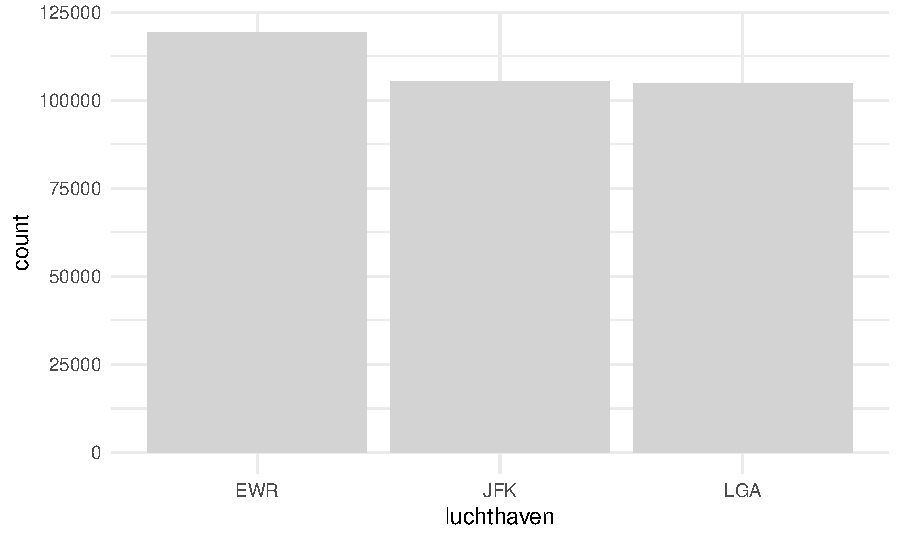
\includegraphics[width=1\linewidth]{textbook_files/figure-latex/2-3a-1} \caption[Staafdiagram luchthavens]{Staafdiagram luchthavens}\label{fig:2-3a}
\end{figure}

\begin{itemize}
\tightlist
\item
  Minder geschikt indien er veel waarden zijn. Dan wordt de X-as snel onleesbaar.(Fig. \ref{fig:2-3b})
\end{itemize}

\begin{figure}
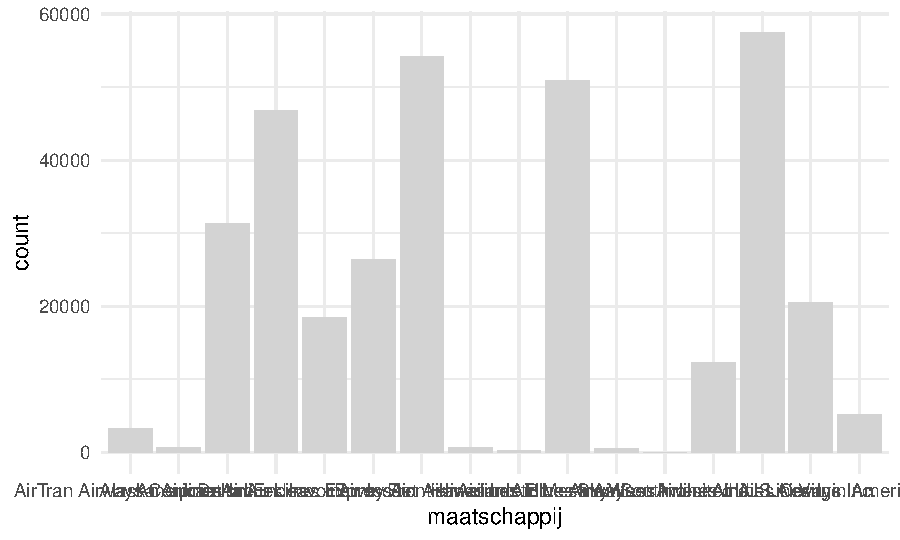
\includegraphics[width=1\linewidth]{textbook_files/figure-latex/2-3b-1} \caption[Staafdiagram maatschappijen]{Staafdiagram maatschappijen}\label{fig:2-3b}
\end{figure}

\begin{itemize}
\tightlist
\item
  Je kan natuurlijk de labels roteren. Maar dit kan nog steeds onhandig zijn om te lezen. (Fig. \ref{fig:2-3c}).
\end{itemize}

\begin{figure}
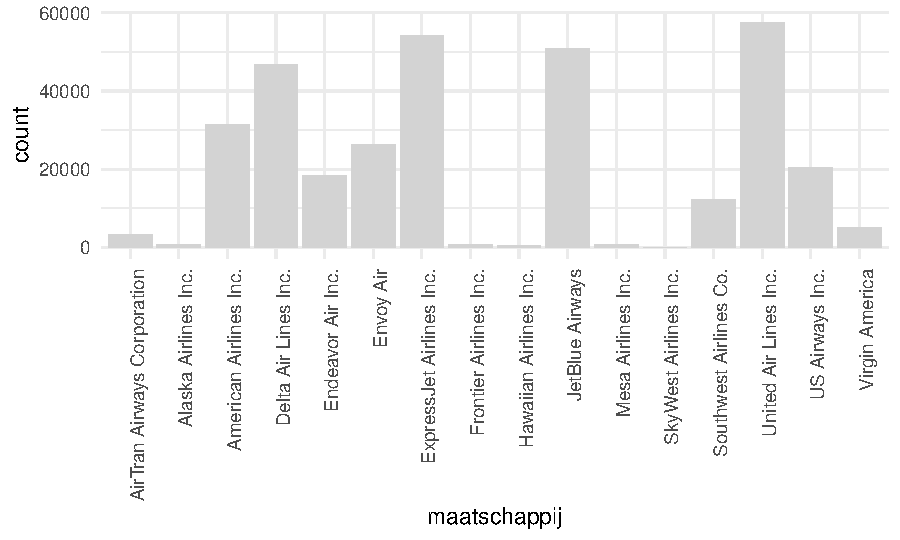
\includegraphics[width=1\linewidth]{textbook_files/figure-latex/2-3c-1} \caption[Staafdiagram met geroteerde labels]{Staafdiagram met geroteerde labels}\label{fig:2-3c}
\end{figure}

\begin{itemize}
\tightlist
\item
  In geval van een \textbf{nominale} variabele zijn er twee mogelijkheden om de waarden te rangschikken:

  \begin{itemize}
  \tightlist
  \item
    Alfabetisch. (standaard) Dit is handig om snel waarden terug te vinden.
  \item
    Volgens frequentie. Dit is handig om snel te zien welke waarden vaak/weinig voorkomen en geeft ook een beter beeld van de verdeling van de waarden. (Fig. \ref{fig:2-3d})
  \end{itemize}
\end{itemize}

\begin{figure}
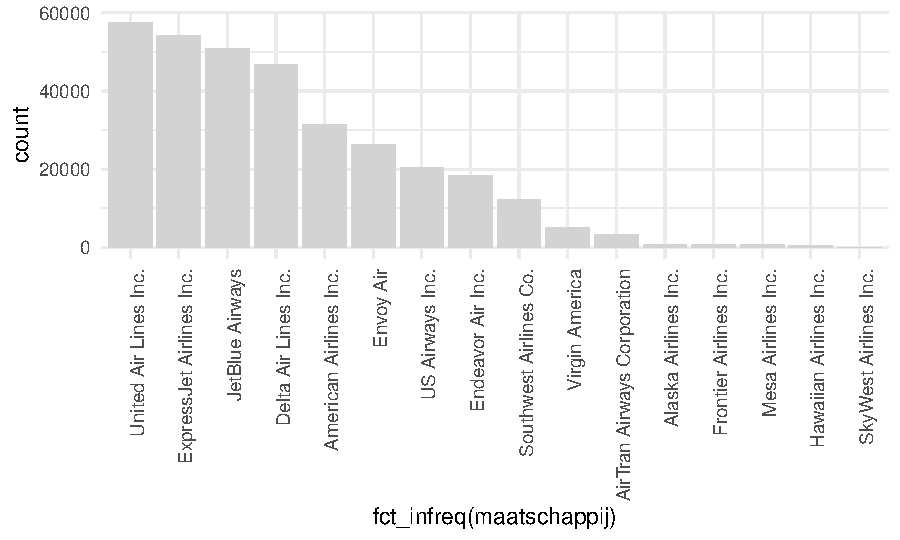
\includegraphics[width=1\linewidth]{textbook_files/figure-latex/2-3d-1} \caption[Staafdiagram gesorteerd op frequentie]{Staafdiagram gesorteerd op frequentie}\label{fig:2-3d}
\end{figure}

\begin{itemize}
\item
  In het geval van een \textbf{ordinale} variabele houd je best de intrinsieke volgorde van de waarden aan.
\item
  Je kan ook een horizontaal staafdiagram maken. (Fig. \ref{fig:2-3e})

  \begin{itemize}
  \tightlist
  \item
    Zelfde principe, maar dan met horizontale balken.
  \item
    Is handiger om de verschillende waarden te lezen, vooral indien dit er veel zijn.
  \end{itemize}
\end{itemize}

\begin{figure}
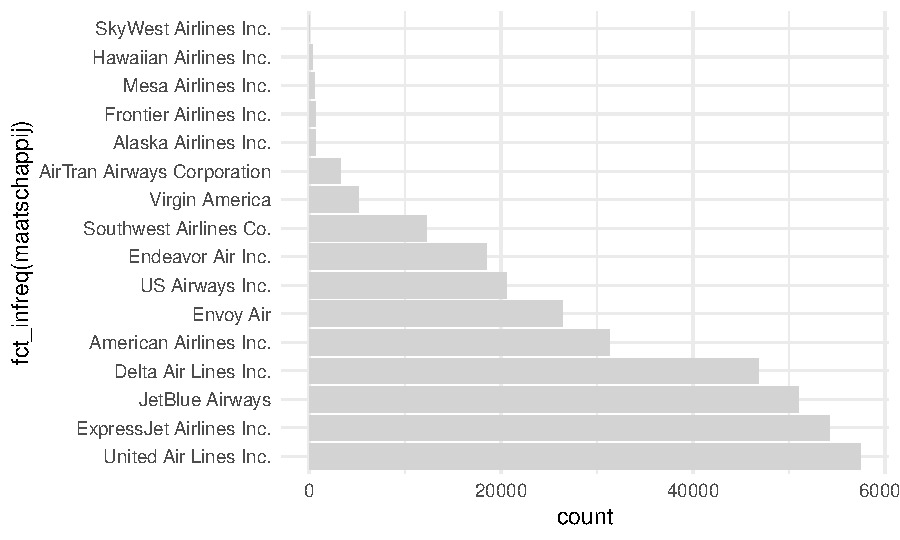
\includegraphics[width=1\linewidth]{textbook_files/figure-latex/2-3e-1} \caption[Verticaal staafdiagram gesorteerd op frequentie]{Verticaal staafdiagram gesorteerd op frequentie}\label{fig:2-3e}
\end{figure}

\hypertarget{dotplot}{%
\subsubsection{Dotplot}\label{dotplot}}

\begin{itemize}
\item
  In plaats van balken te gebruiken om de frequentie van een waarde aan te geven, kan je dit ook met punten doen. (Fig. \ref{fig:2-5a})
\item
  Een dotplot laat duidelijker zien waar de sprongen in de verdeling zit. Daarom is de dotplot vooral relevant als je de waarden ordent volgens frequentie.

  \begin{figure}
  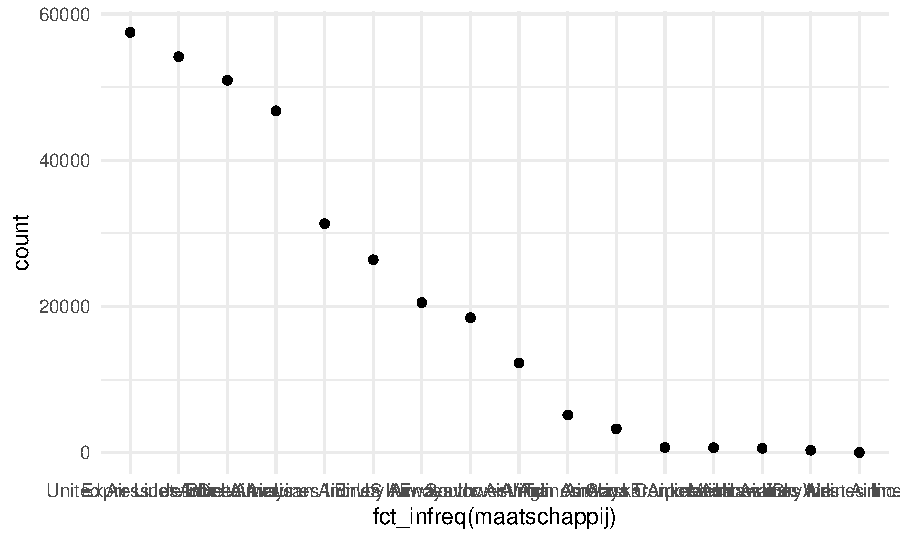
\includegraphics[width=1\linewidth]{textbook_files/figure-latex/2-5a-1} \caption[Dotplot maatschappij]{Dotplot maatschappij}\label{fig:2-5a}
  \end{figure}
\item
  Net als de barplot kan je zowel een verticale als horizontale dotplot maken. (Fig. \ref{fig:2-5b})
\end{itemize}

\begin{figure}
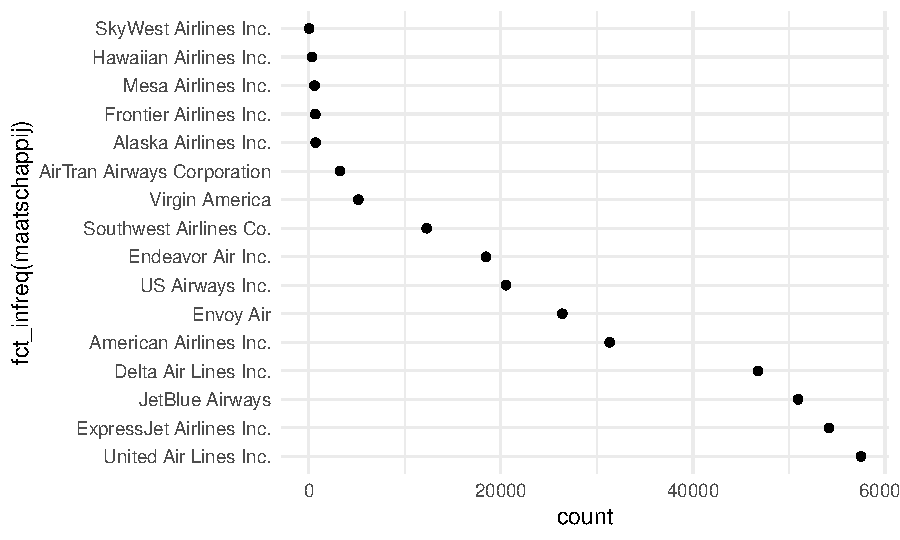
\includegraphics[width=1\linewidth]{textbook_files/figure-latex/2-5b-1} \caption[Verticale dotplot]{Verticale dotplot}\label{fig:2-5b}
\end{figure}

\hypertarget{stacked-staafdiagram}{%
\subsubsection{`Stacked' staafdiagram}\label{stacked-staafdiagram}}

\begin{itemize}
\tightlist
\item
  We maken nu slechts 1 kolom. Iedere waarde is een andere kleur en neemt een deel van de balk in beslag. De volledige balk stelt 100\% van de data voor. (Fig. \ref{fig:2-6a})
\item
  Kan nuttig zijn om data cumulatief te bestuderen.
\item
  Hiermee kunnen we vragen beantwoorden zoals: ``Welke waarden moeten we nemen om met zo weinig mogelijk waarden x\% van de objecten te hebben?''
\end{itemize}

\begin{figure}

{\centering 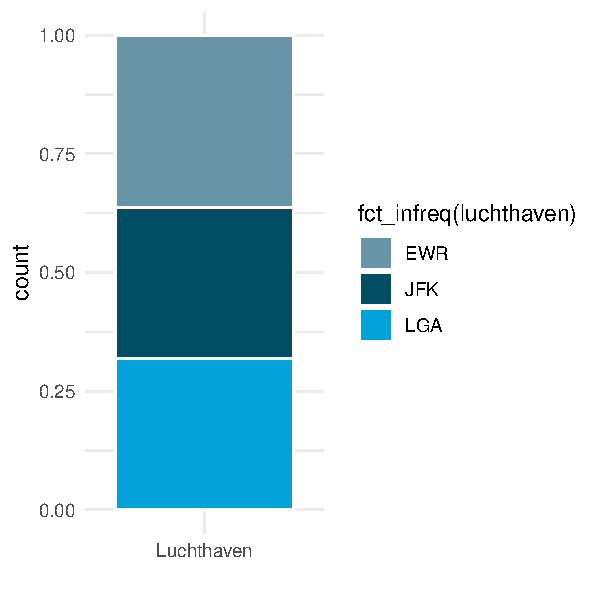
\includegraphics[width=0.7\linewidth]{textbook_files/figure-latex/2-6a-1} 

}

\caption[Stacked barplot]{Stacked barplot}\label{fig:2-6a}
\end{figure}

\begin{itemize}
\tightlist
\item
  We kunnen ook horizontale versies maken. (Fig. \ref{fig:2-6b})
\end{itemize}

\begin{figure}
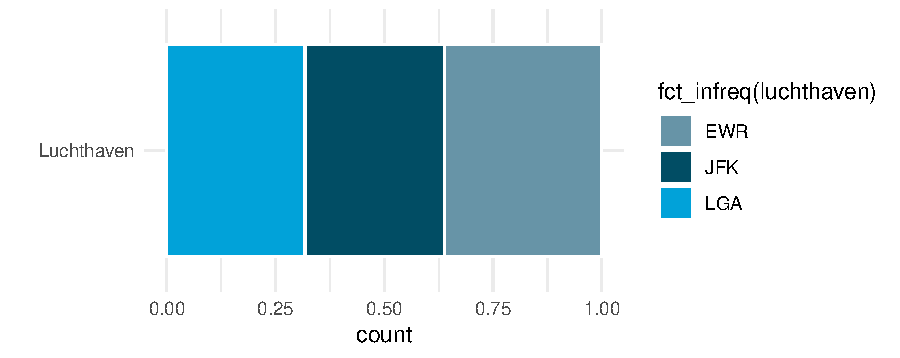
\includegraphics[width=1\linewidth]{textbook_files/figure-latex/2-6b-1} \caption[Horizontale stacked barplot]{Horizontale stacked barplot}\label{fig:2-6b}
\end{figure}

\begin{itemize}
\tightlist
\item
  Univariate stacked barcharts kunnen soms wat \emph{raar} overkomen. Vaak komt een gewone barchart beter over.
\end{itemize}

\hypertarget{andere-soorten}{%
\subsubsection{Andere soorten}\label{andere-soorten}}

\begin{itemize}
\tightlist
\item
  treemap: indelen van rechthoekige oppervlakte volgens categorische variabelen
\item
  pie chart

  \begin{itemize}
  \tightlist
  \item
    Moeilijk te interpreteren.
  \item
    Verschillen tussen waarden zijn enkel duidelijk bij grote verschillen, terwijl barplots en dotplots deze ook bij kleine verschillen kunnen tonen.
  \item
    Voor cumulatieve analyses van de data zijn barplots beter omdat het hier eenvoudiger is om af te leiden waar x\% zicht bevindt.
  \end{itemize}
\end{itemize}

\hypertarget{continue-variabele}{%
\subsection{Continue variabele}\label{continue-variabele}}

\hypertarget{histogram}{%
\subsubsection{Histogram}\label{histogram}}

\begin{itemize}
\tightlist
\item
  Analoog met barplot, alleen gaan we hier eerst onze ``categorieën'' definiëren. (Fig. \ref{fig:2-7a})
\item
  Dit wordt `binning' genoemd en wordt bepaald door een bin-breedte te kiezen.
\item
  Je kan de binbreedte rechtstreeks kiezen of bepalen door vast te leggen hoeveel categorieën/bins je wenst.
\end{itemize}

\begin{figure}
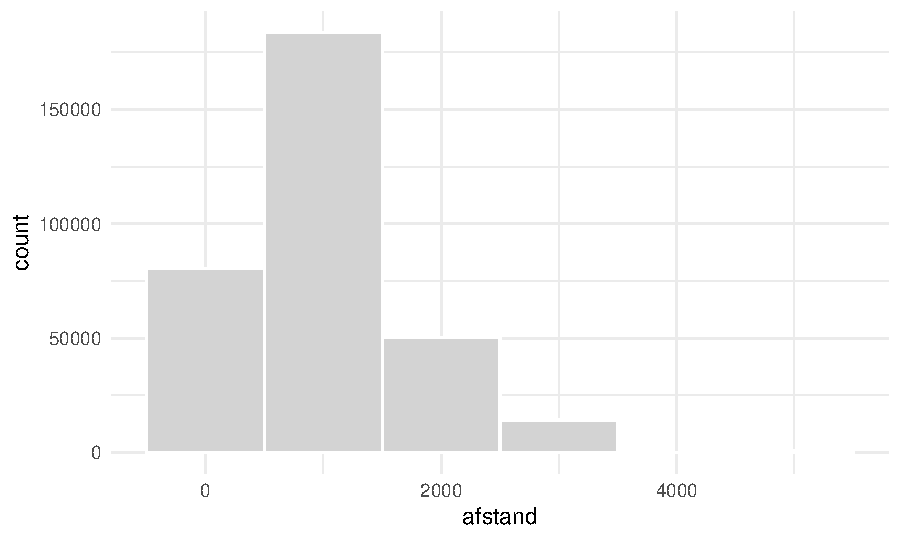
\includegraphics[width=1\linewidth]{textbook_files/figure-latex/2-7a-1} \caption[Histogram with binwidth 1000]{Histogram with binwidth 1000}\label{fig:2-7a}
\end{figure}

\begin{itemize}
\tightlist
\item
  Voor de visualisatie, worden alle waarden gegroepeerd per `bin'.
\item
  De binbreedte kan een enorme impact hebben op het uitzicht van de verdeling. (Fig. \ref{fig:2-7b} - \ref{fig:2-7c})

  \begin{itemize}
  \tightlist
  \item
    Hoe breder de bins, hoe minder modi je kan detecteren.
  \item
    Hoe smaller de bins, hoe meer modi je gaat zien, hoewel dit niet altijd even betekenisvol is.
  \item
    Hoe smaller de bins, hoe minder data er in iedere bin gaat zitten en dan kunnen patronen wel in jouw dataset bestaan maar louter ten gevolge van toeval.
  \end{itemize}
\end{itemize}

\begin{figure}
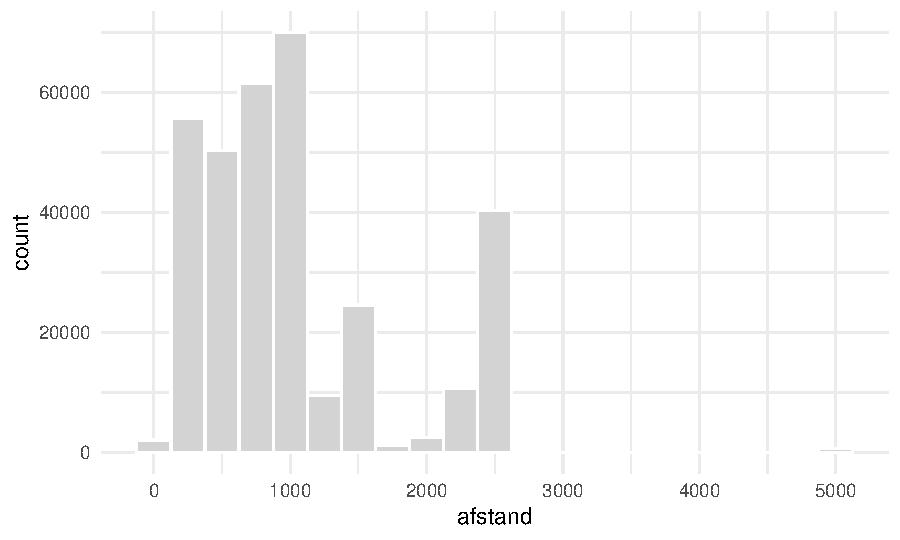
\includegraphics[width=1\linewidth]{textbook_files/figure-latex/2-7b-1} \caption[Histogram with binwidth 250]{Histogram with binwidth 250}\label{fig:2-7b}
\end{figure}

\begin{figure}
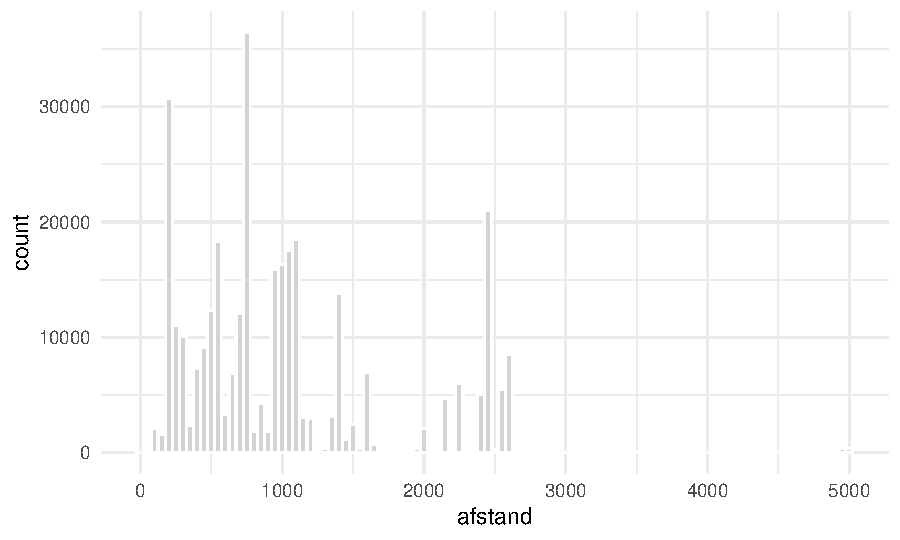
\includegraphics[width=1\linewidth]{textbook_files/figure-latex/2-7c-1} \caption[Histogram with binwidth 50]{Histogram with binwidth 50}\label{fig:2-7c}
\end{figure}

\hypertarget{density}{%
\subsubsection{Density}\label{density}}

\begin{itemize}
\tightlist
\item
  Variant van histogram.
\item
  In plaats van staven wordt er een curve getekend. (Fig. \ref{fig:2-density})
\item
  De oppervlakte onder de curve is steeds gelijk aan 1
\item
  Hoe hoger de curve, hoe meer observaties ter hoogt van deze waarde (hoe hoger de densiteit)
\item
  De waarde van de y-as heeft geen directe betekenis.
\end{itemize}

\begin{figure}
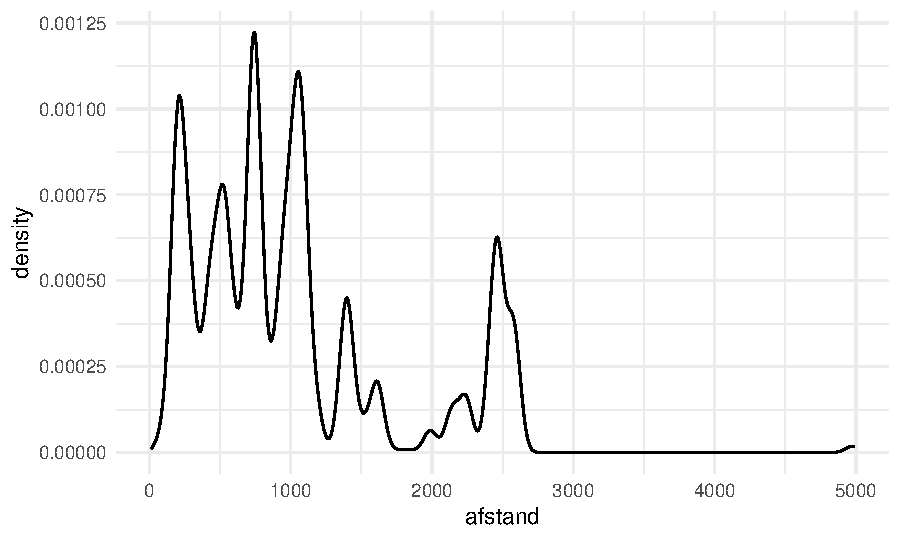
\includegraphics[width=1\linewidth]{textbook_files/figure-latex/2-density-1} \caption[Density plot]{Density plot}\label{fig:2-density}
\end{figure}

\hypertarget{boxplot}{%
\subsubsection{Boxplot}\label{boxplot}}

\begin{itemize}
\tightlist
\item
  De lijn in het midden duidt de mediaan aan. Dit betekent dat 50\% van je data onder deze lijn ligt, terwijl 50\% er boven ligt. (Fig. \ref{fig:2-8})
\item
  De box in het midden duidt de middelste 50\% van je data aan. Dit wordt ook de interkwartiel-box genoemd. Dit betekent dat 25\% van je data onder deze box zit en nog eens 25\% boven deze box ligt. Hoe groter de box, des te meer de data gespreid is.
\item
  Indien de box aan één zijde van de mediaanlijn groter is dan aan de andere zijde, dan wijst dit er op dat de data meer gespreid is aan die kant.
\item
  De ``whiskers'' geven de laatste datapunten aan die als ``normaal'' beschouwd worden. Datapunten buiten deze grenzen beschouwt een boxplot als outliers of extreme waarden.
\item
  De grens waar data van normaal naar extreem overgaat wordt door de boxplot bepaald door anderhalf keer de grootte van de interkwartiel-box op te tellen (en af te trekken) van de bovenste (onderste) grens van de interkwartiel-box. Punten die hier buiten liggen zijn outliers en worden als aparte punten aangeduid. De uitersten van de whiskers duiden de laatste datapunten aan binnen deze grenzen.
\end{itemize}

\begin{figure}

{\centering 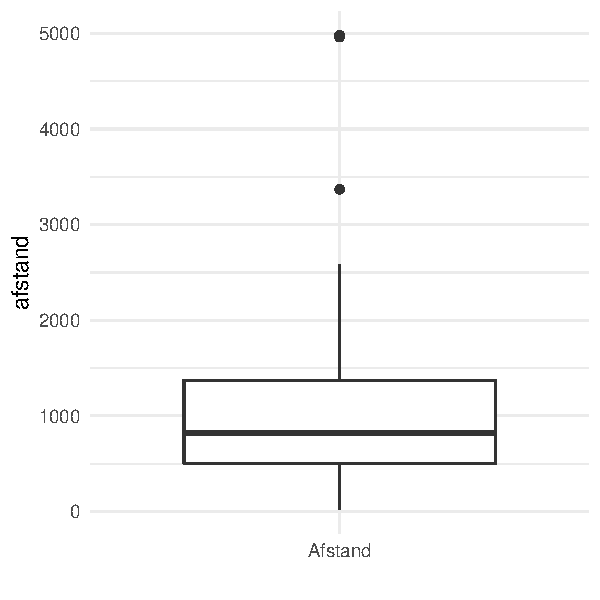
\includegraphics[width=0.7\linewidth]{textbook_files/figure-latex/2-8-1} 

}

\caption[Verticale boxplot vertrekvertraging]{Verticale boxplot vertrekvertraging}\label{fig:2-8}
\end{figure}

\begin{itemize}
\tightlist
\item
  Het is niet abnormaal dat er outliers in je data aanwezig zijn.
\item
  Bij normaal verdeelde data zal je gemiddeld 7 outliers per 1000 datapunten mogen verwachten.

  \begin{itemize}
  \tightlist
  \item
    Een normale verdeling is een bepaalde manier waarop data waarden verdeeld kunnen zijn die in de realiteit vaak voorkomt.
  \end{itemize}
\item
  Indien je echter veel meer outliers ziet op je boxplot visualisatie, dan is de kans reëel dat er meer aan de hand is:

  \begin{itemize}
  \tightlist
  \item
    Er zijn bijvoorbeeld systematische meetfouten
  \item
    De objecten in je data zijn in feite op bepaalde aspecten significant verschillend waardoor je ze apart zou moeten bestuderen.
  \end{itemize}
\item
  Je kan een boxplot ook roteren. (Fig \ref{fig:2-9})
\item
  Boxplots komen beter tot hun recht bij bivariate analyses dan bij univariate analyses.
\end{itemize}

\begin{figure}
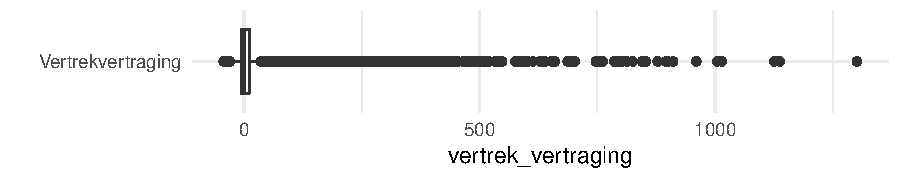
\includegraphics[width=1\linewidth]{textbook_files/figure-latex/2-9-1} \caption[Horizontale boxplot vertrekvertraging]{Horizontale boxplot vertrekvertraging}\label{fig:2-9}
\end{figure}

\hypertarget{violin-plot}{%
\subsubsection{Violin plot}\label{violin-plot}}

\begin{itemize}
\tightlist
\item
  Een violin plot kan je beschouwen als een combinatie van een histogram en een boxplot. (Fig. @ref(fig:2\_10a))
\item
  Net als bij een boxplot wordt op verticale wijze getoond hoe de data verspreid is.
\item
  Opnieuw kan je ervoor kiezen de grafiek te roteren. (Fig. @ref(fig:2\_10b))
\item
  Net als bij een histogram kan je goed zien waar het volume (de massa) van de data zich bevindt.
\item
  Net als bij een histogram kan je detecteren hoeveel modi de data bezit.
\item
  In tegenstelling tot de boxplot, kan je bij een violinplot wel niet duidelijk zien waar bijvoorbeeld het `midden' van je data is.
\end{itemize}

\begin{figure}

{\centering 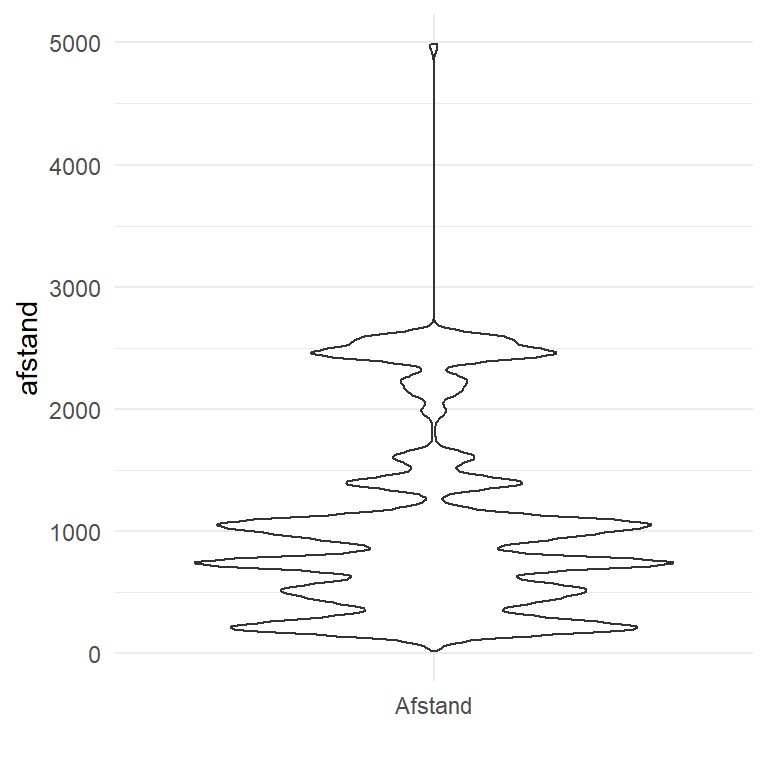
\includegraphics[width=0.7\linewidth]{textbook_files/figure-latex/2-10a-1} 

}

\caption[Verticale violin plot afstand]{Verticale violin plot afstand}\label{fig:2-10a}
\end{figure}

\begin{figure}
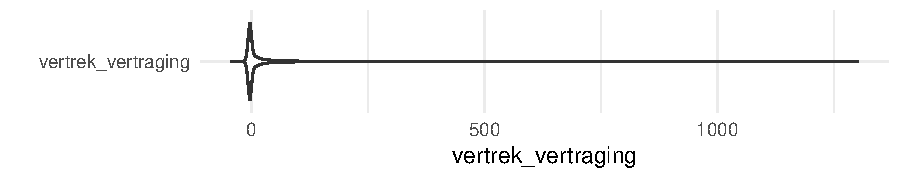
\includegraphics[width=1\linewidth]{textbook_files/figure-latex/2-10b-1} \caption[Horizontale violin plot vertrekvertraging]{Horizontale violin plot vertrekvertraging}\label{fig:2-10b}
\end{figure}

\hypertarget{jitter-plot}{%
\subsubsection{Jitter plot}\label{jitter-plot}}

\begin{itemize}
\tightlist
\item
  puntenwolk waarbij willekeurige ``noise'' (ruis) wordt toegevoegd.
\item
  de ruis zorgt ervoor dat datapunten niet overlappen, en dat het duidelijk is waar de massa zich bevindt.
\item
  Fig. \ref{fig:2-jitter} toont een vergelijking van violin, boxplot, point en jitter plot.
\end{itemize}

\begin{figure}
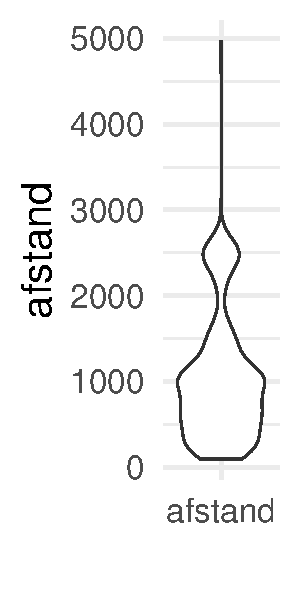
\includegraphics[width=0.24\linewidth]{textbook_files/figure-latex/2-jitter-1} 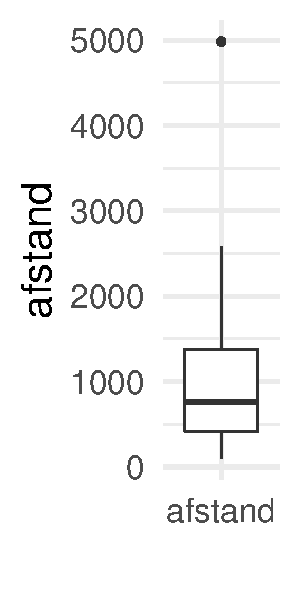
\includegraphics[width=0.24\linewidth]{textbook_files/figure-latex/2-jitter-2} 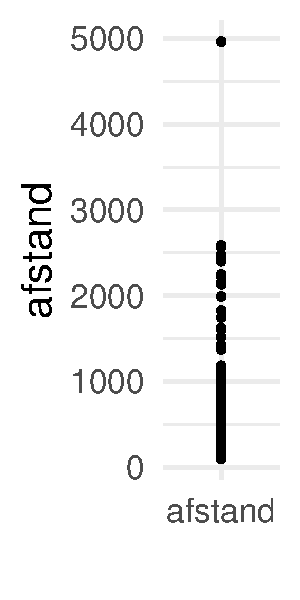
\includegraphics[width=0.24\linewidth]{textbook_files/figure-latex/2-jitter-3} 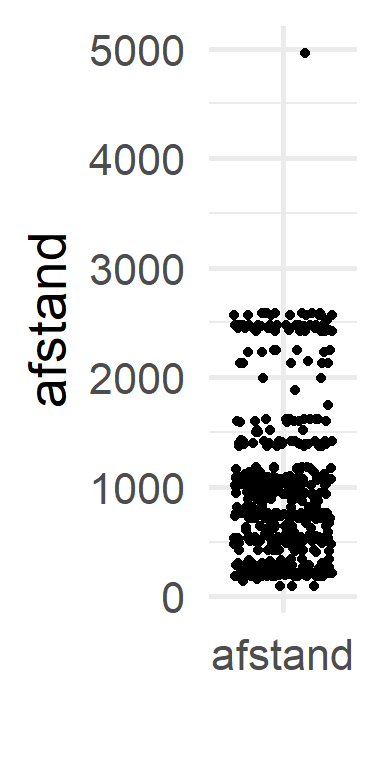
\includegraphics[width=0.24\linewidth]{textbook_files/figure-latex/2-jitter-4} \caption[Violin, boxplot, point en jitter]{Violin, boxplot, point en jitter}\label{fig:2-jitter}
\end{figure}

\hypertarget{bivariate-visualisatie-2-variabelen}{%
\section{Bivariate visualisatie (2 variabelen)}\label{bivariate-visualisatie-2-variabelen}}

\begin{itemize}
\tightlist
\item
  Wanneer we de relatie tussen 2 variabelen bekijken is het eenvoudig te denken in \emph{oorzaak} en gevolg \emph{termen.} \footnote{Zie opmerking i.v.m. correlatie versus causaliteit, \ref{how-charts-lie}.}

  \begin{itemize}
  \tightlist
  \item
    De variabele die we het label ``oorzaak'' geven, zullen we voortaan ``onafhankelijke variabele'' noemen.
  \item
    De variabele die we het label ``gevolg'' geven, zullen we voortaan ``afhankelijke variabele'' noemen.
  \end{itemize}
\item
  Waar we eigenlijk in geïnteresseerd zijn bij een visualisatie van 2 variabelen is de impact van de onafhankelijke variabele op de afhankelijke variabele weer te geven.
\item
  Alle vragen die we kunnen stellen bij de visualisatie van één variabele, kunnen we nog steeds stellen, met telkens de bijkomende vraag of het waargenomen patroon verandert als de onafhankelijke variabele van waarde verandert.
\end{itemize}

\hypertarget{situatie-1-de-onafhankelijke-variabele-is-categorisch}{%
\subsection{Situatie 1: De onafhankelijke variabele is categorisch}\label{situatie-1-de-onafhankelijke-variabele-is-categorisch}}

Indien de afhankelijke variabele een continue variabele is kan je:

\begin{itemize}
\tightlist
\item
  meerdere boxplots op 1 grafiek visualiseren, met telkens 1 boxplot per waarde van de onafhankelijke variabele. (Fig. \ref{fig:2-12a})
\end{itemize}

\begin{figure}
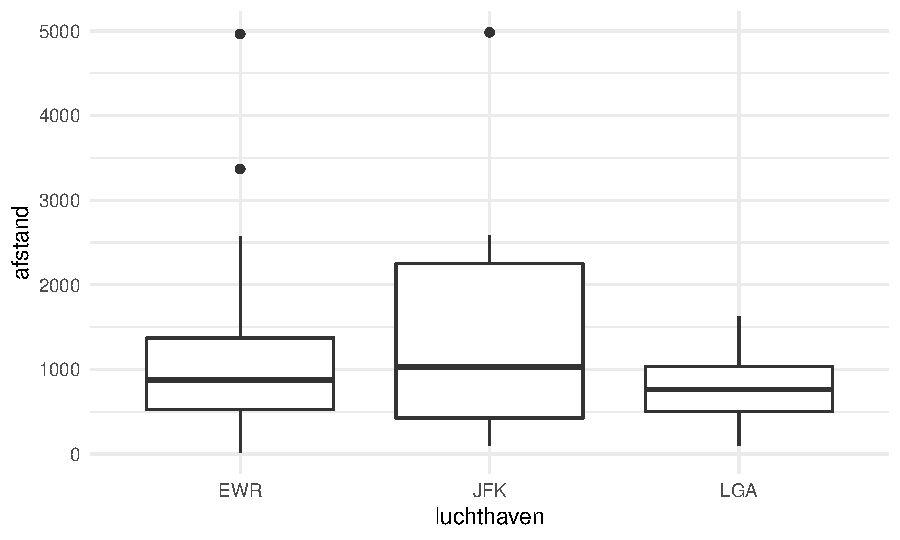
\includegraphics[width=1\linewidth]{textbook_files/figure-latex/2-12a-1} \caption[Bivariate boxplot]{Bivariate boxplot}\label{fig:2-12a}
\end{figure}

\begin{itemize}
\tightlist
\item
  meerdere violinplots op 1 grafiek tonen, met telkens 1 violinplot per waarde van de onafhankelijke variabele. (Fig. \ref{fig:2-12b})
\end{itemize}

\begin{figure}
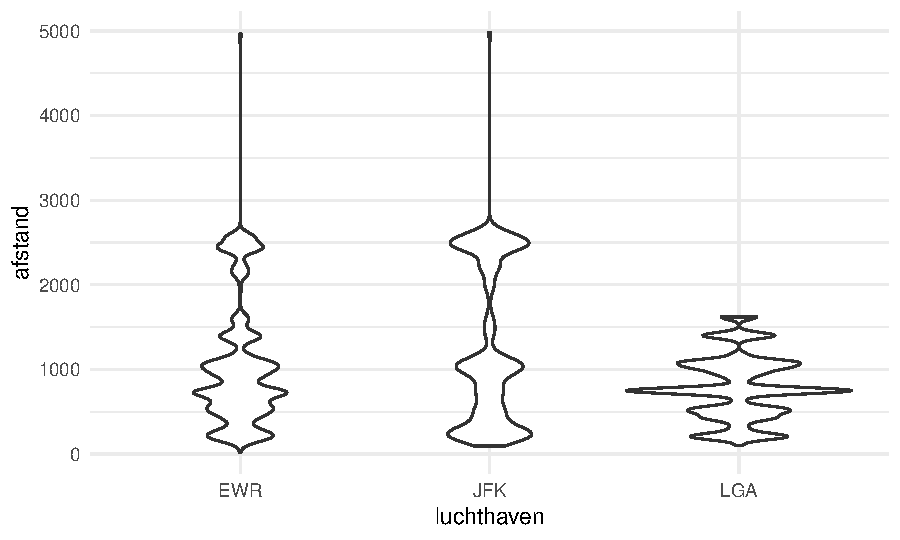
\includegraphics[width=1\linewidth]{textbook_files/figure-latex/2-12b-1} \caption[Bivariate violin plot]{Bivariate violin plot}\label{fig:2-12b}
\end{figure}

\begin{itemize}
\tightlist
\item
  meerdere histogrammen op 1 grafiek tonen

  \begin{itemize}
  \tightlist
  \item
    Hiervoor gebruiken we facetten: we tekenen voor elke waarde van de onafhankelijke variabele een apart assenstelsel. (Fig. \ref{fig:2-12c})
  \end{itemize}
\end{itemize}

\begin{figure}
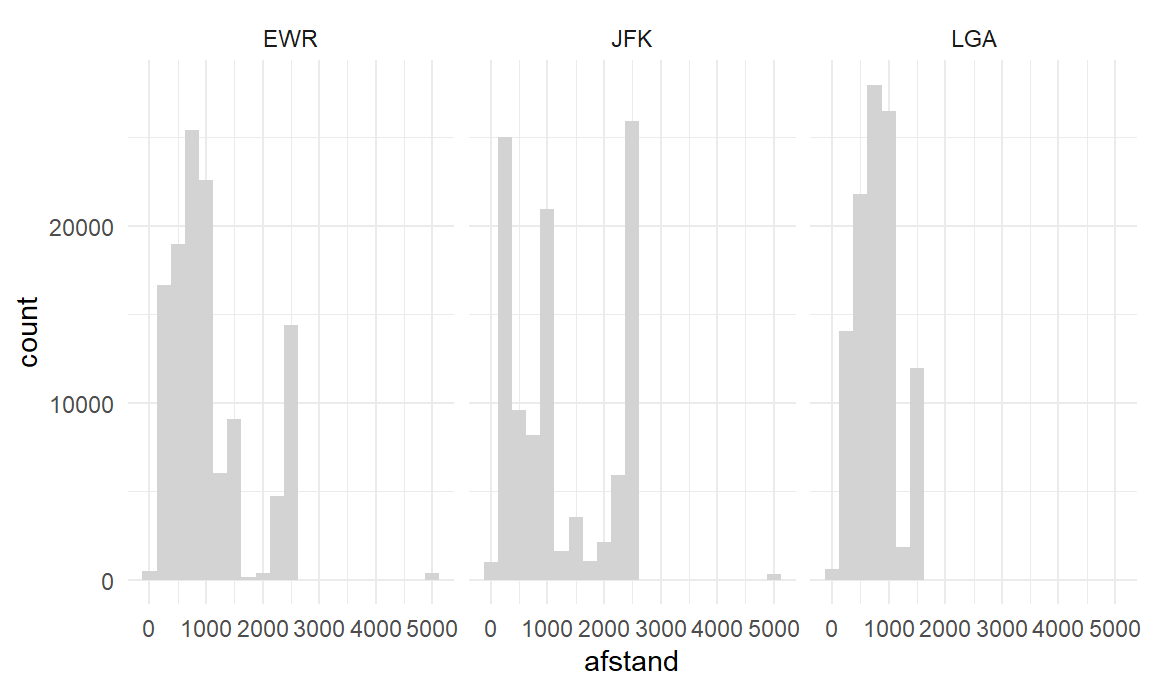
\includegraphics[width=1\linewidth]{textbook_files/figure-latex/2-12c-1} \caption[Bivariate histogram plot]{Bivariate histogram plot}\label{fig:2-12c}
\end{figure}

\begin{itemize}
\tightlist
\item
  meerdere density plots
\item
  Hiervoor kunnen we facetten gebruiken, ofwel de density plots over elkaar tekenen en onderscheiden met kleur. (Fig. \ref{fig:2-12d}-\ref{fig:2-12e})
\end{itemize}

\begin{figure}
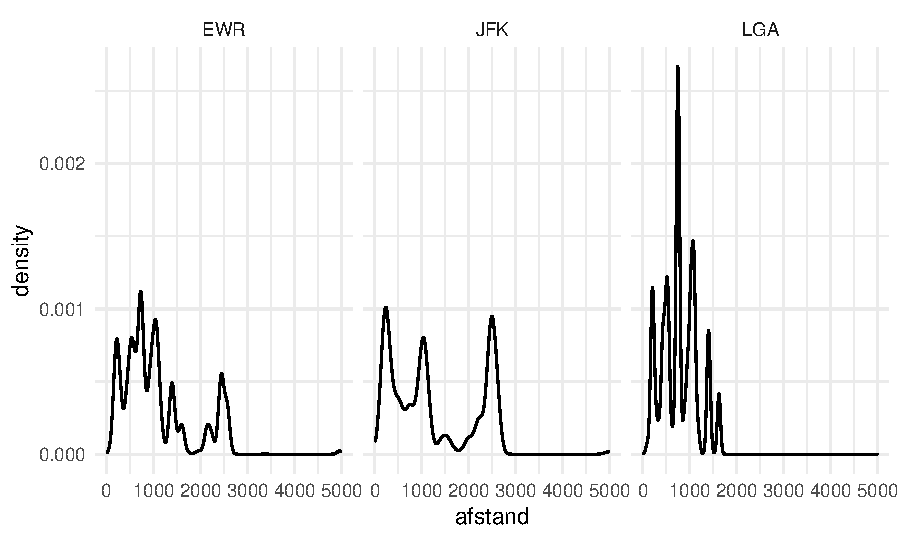
\includegraphics[width=1\linewidth]{textbook_files/figure-latex/2-12d-1} \caption[Bivariate density plot - apart]{Bivariate density plot - apart}\label{fig:2-12d}
\end{figure}

\begin{figure}
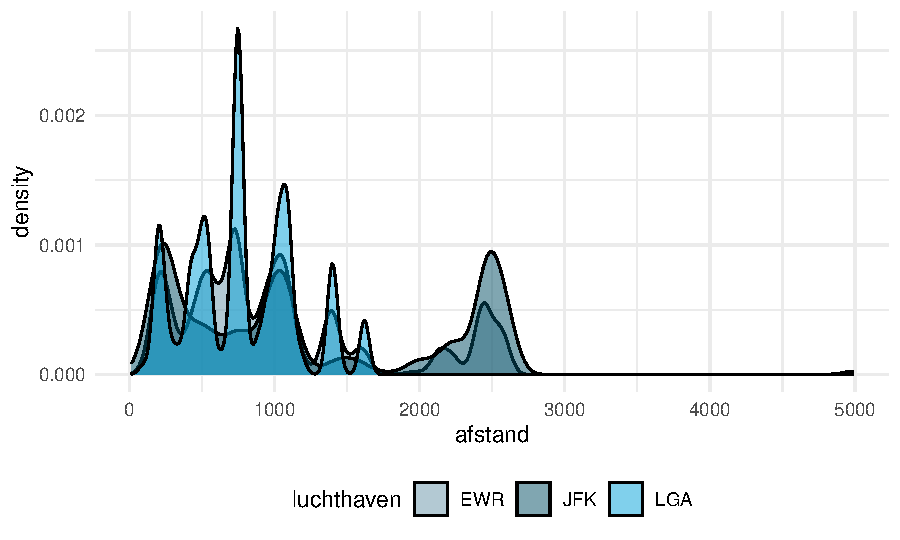
\includegraphics[width=1\linewidth]{textbook_files/figure-latex/2-12e-1} 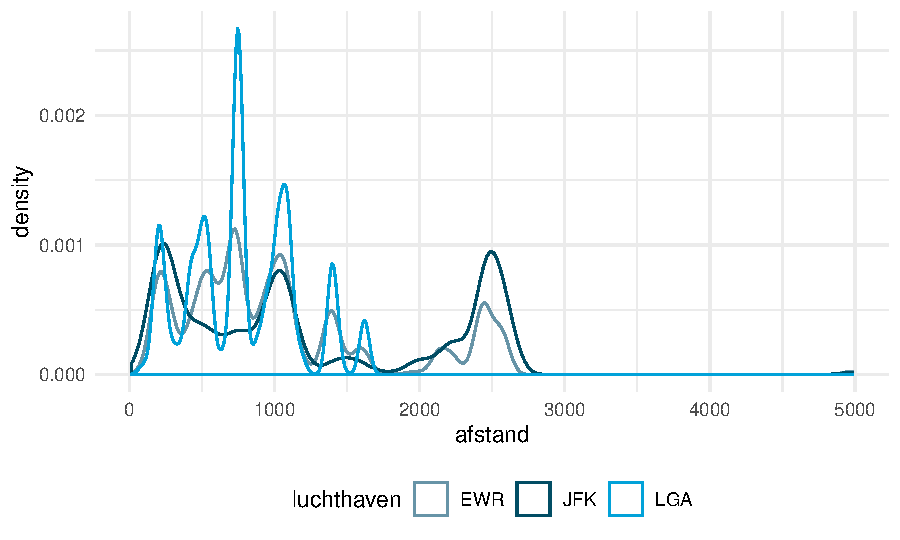
\includegraphics[width=1\linewidth]{textbook_files/figure-latex/2-12e-2} \caption[Bivariate density plot - overlappend]{Bivariate density plot - overlappend}\label{fig:2-12e}
\end{figure}

Indien de afhankelijke variabele een \textbf{categorische variabele} is:

\begin{itemize}
\tightlist
\item
  Kan je meerdere barplots op 1 grafiek visualiseren, met telkens de bars gegroepeerd per waarde van de onafhankelijke variabele.
\end{itemize}

\begin{figure}
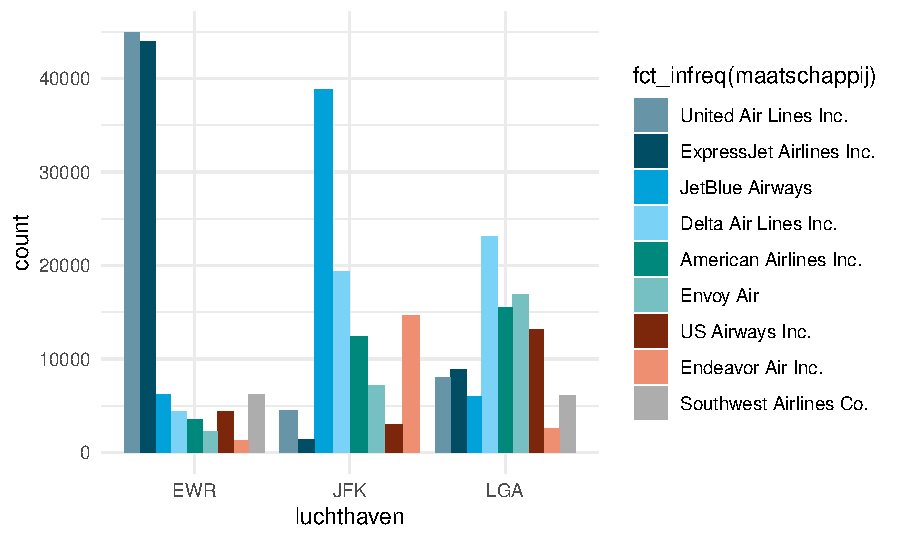
\includegraphics[width=1\linewidth]{textbook_files/figure-latex/2-13a-1} \caption[Bivariate barplot]{Bivariate barplot}\label{fig:2-13a}
\end{figure}

\begin{itemize}
\tightlist
\item
  Kan je meerdere stacked barplots op 1 grafiek plaatsen, met telkens een volledige stack per waarde van de onafhankelijke variabele.
\end{itemize}

\begin{figure}
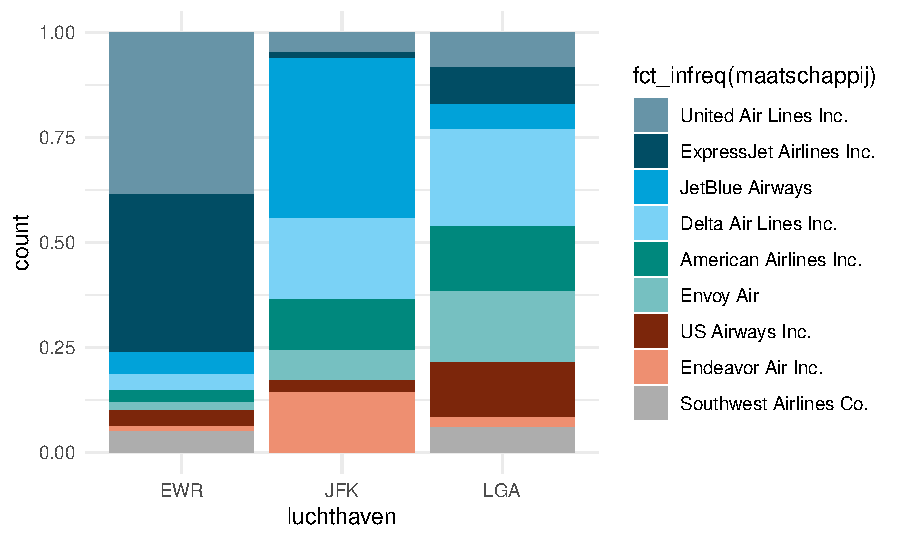
\includegraphics[width=1\linewidth]{textbook_files/figure-latex/2-13b-1} \caption[Bivariate stacked barplot]{Bivariate stacked barplot}\label{fig:2-13b}
\end{figure}

\begin{itemize}
\tightlist
\item
  Kan je een heatmap (of tile plot) gebruiken. Hier bij plaats je 2 categorische variabelen op de x-as en y-as, respectivelijk.

  \begin{itemize}
  \tightlist
  \item
    Voor elke combinatie van waarden is er een tegel die je kan inkleuren volgens de frequentie van de combinatie.
  \end{itemize}
\end{itemize}

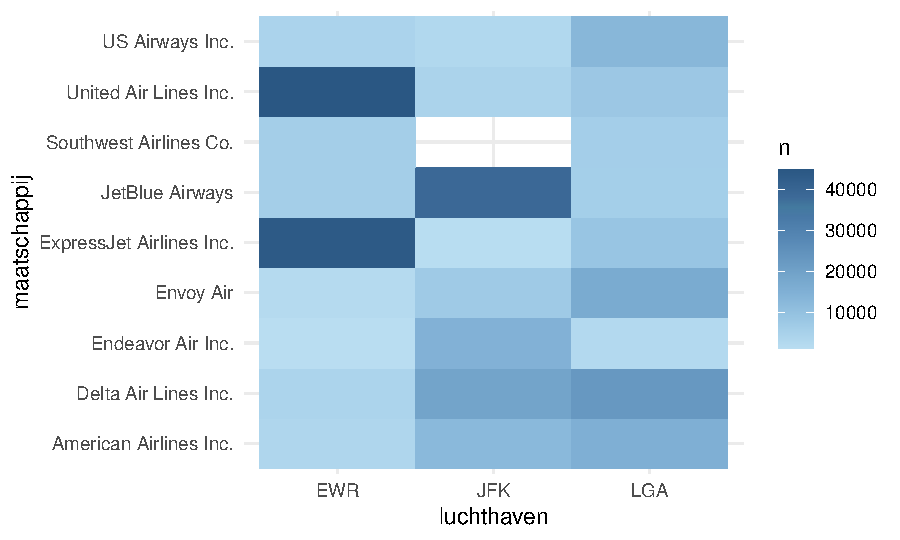
\includegraphics[width=1\linewidth]{textbook_files/figure-latex/unnamed-chunk-7-1}

\begin{itemize}
\tightlist
\item
  Je kan bijkomende ook de exacte waarde in elke tegel plotten.
\end{itemize}

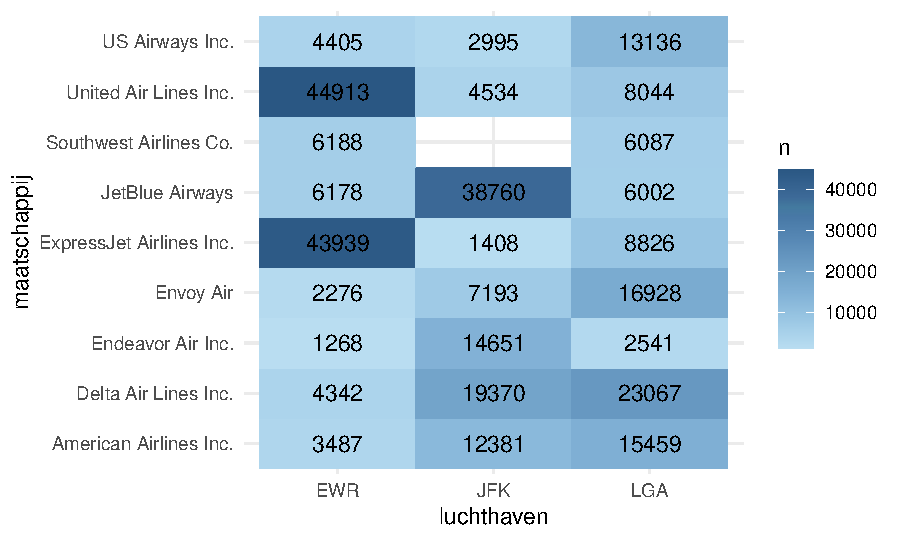
\includegraphics[width=1\linewidth]{textbook_files/figure-latex/unnamed-chunk-8-1}

\textbf{Let op} wanneer beide variabelen categorisch zijn, is het nog steeds van belang welke je beschouwd als afhankelijke en welke als onafhankelijke. Technisch kan je ze omdraaien, maar de betekenis van je visualizatie is niet dezelfde!

\begin{figure}
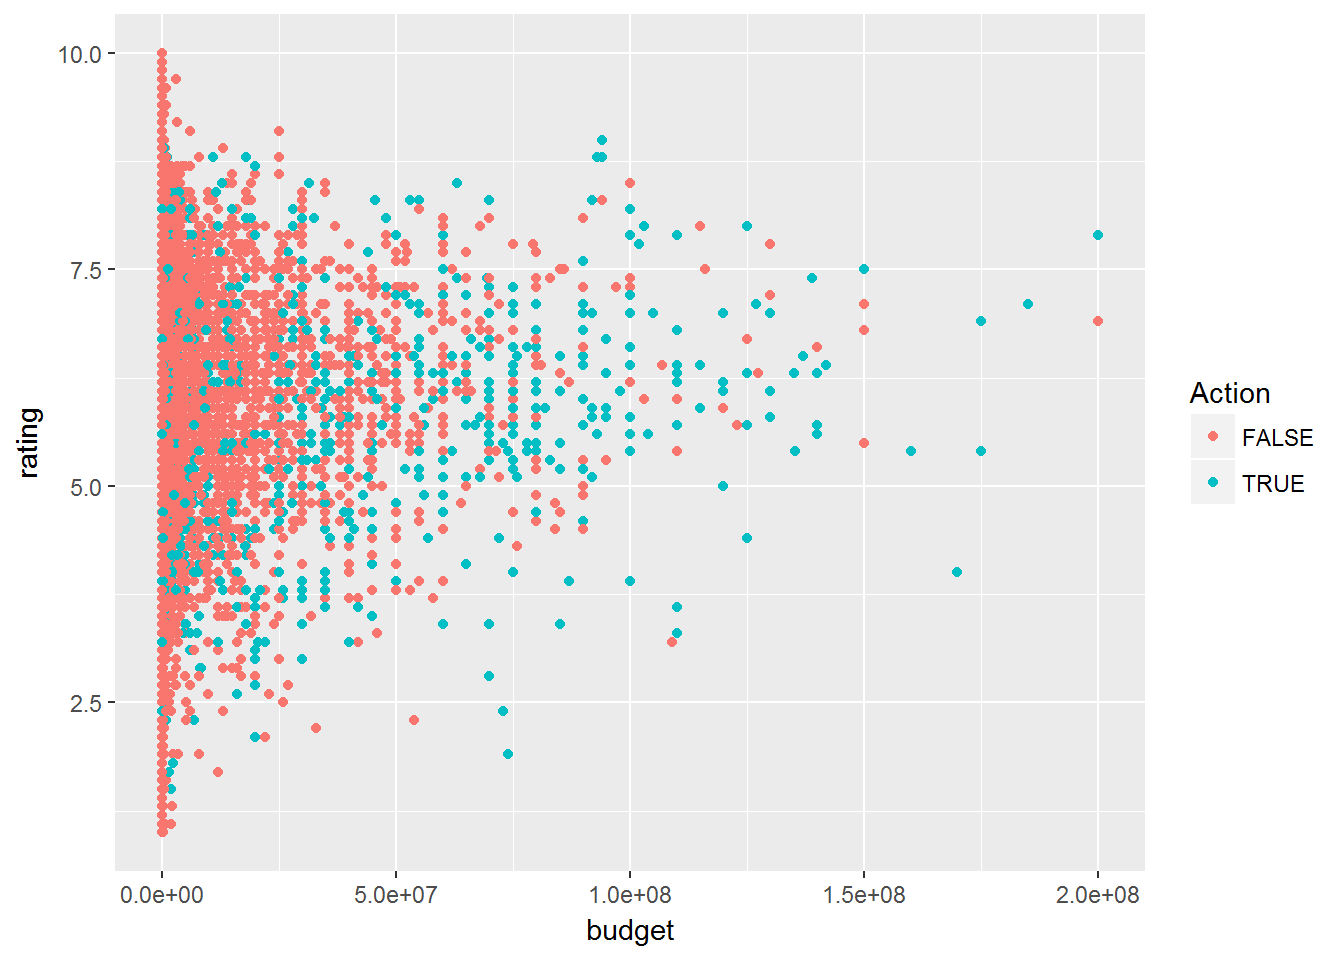
\includegraphics[width=1\linewidth]{textbook_files/figure-latex/unnamed-chunk-9-1} 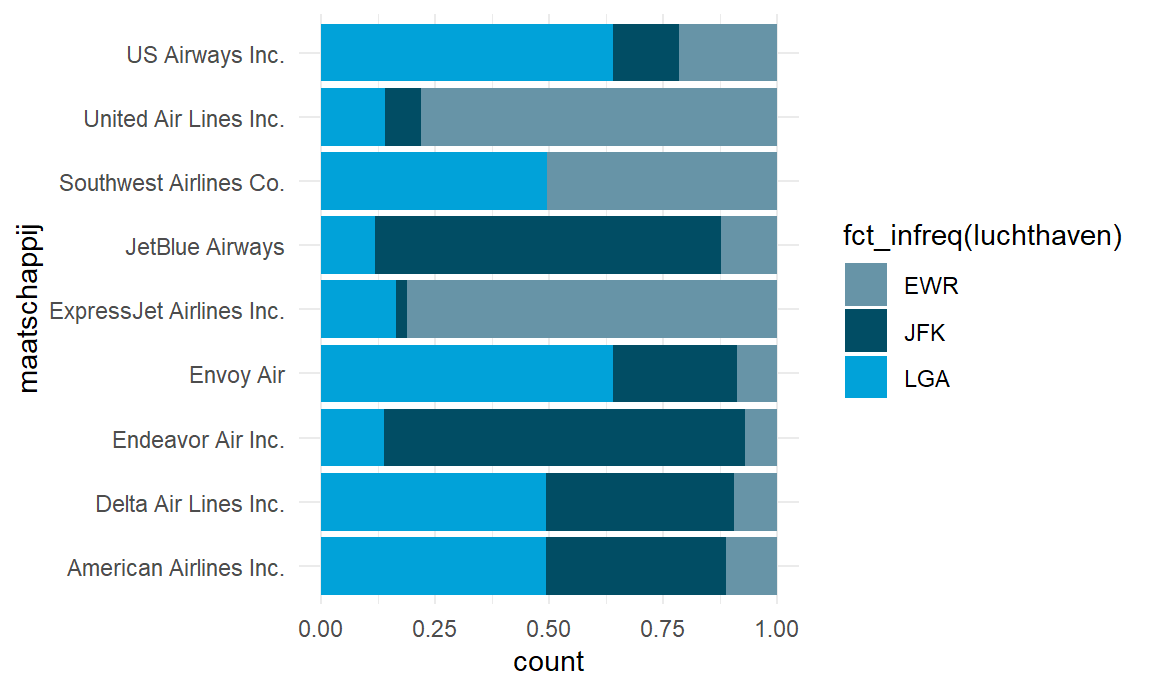
\includegraphics[width=1\linewidth]{textbook_files/figure-latex/unnamed-chunk-9-2} \caption[Twee verschillende stacked barcharts van luchthaven en maatschappij]{Twee verschillende stacked barcharts van luchthaven en maatschappij.}\label{fig:unnamed-chunk-9}
\end{figure}

Andere mogelijkheden:

\begin{itemize}
\tightlist
\item
  treemap (Fig. \ref{fig:treemap})
\end{itemize}

\begin{figure}
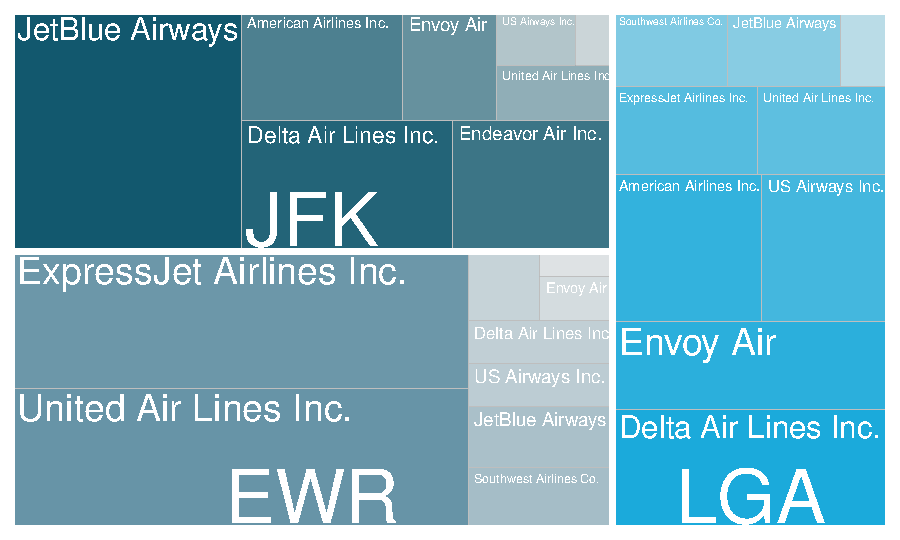
\includegraphics[width=1\linewidth]{textbook_files/figure-latex/treemap-1} \caption[Treemap luchthaven en maatschappij]{Treemap luchthaven en maatschappij.}\label{fig:treemap}
\end{figure}

\begin{itemize}
\tightlist
\item
  mosaic plot (Fig. \ref{fig:mosaic})
\end{itemize}

\begin{figure}
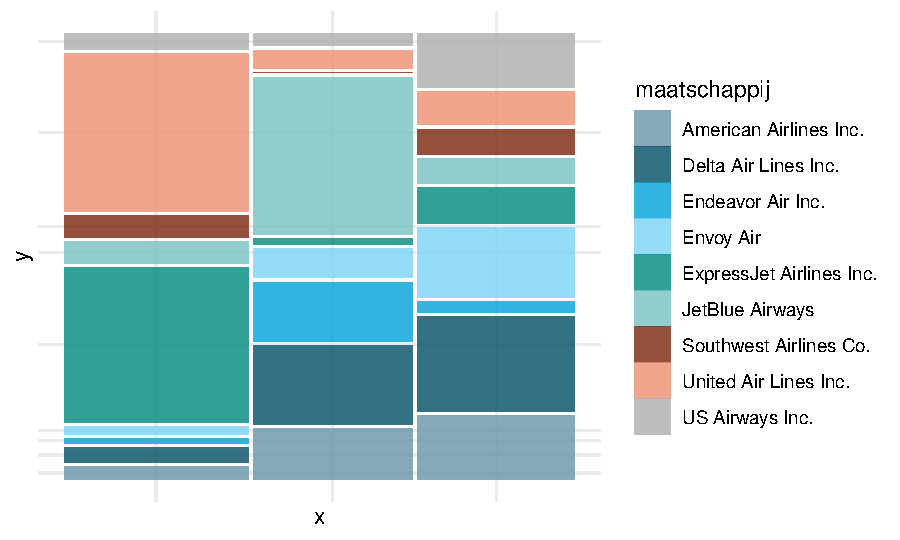
\includegraphics[width=1\linewidth]{textbook_files/figure-latex/mosaic-1} \caption[Mosaic plot luchthaven en maatschappij]{Mosaic plot luchthaven en maatschappij.}\label{fig:mosaic}
\end{figure}

\hypertarget{situatie-2-de-onafhankelijke-variabele-is-continue}{%
\subsection{Situatie 2: De onafhankelijke variabele is continue}\label{situatie-2-de-onafhankelijke-variabele-is-continue}}

\textbf{In dit geval kan je geen aparte plot per mogelijke waarde van de onafhankelijke variabele maken omdat er mogelijk oneindig veel waarden zijn.}

Indien de afhankelijke variabele continu is, dan kan je een scatterplot maken.

\begin{itemize}
\tightlist
\item
  Iedere observatie is een punt in je grafiek, waarbij de x-waarde op de grafiek overeenkomt met de waarde van de onafhankelijke variabele en de y-waarde op de grafiek overeenkomt met de waarde van de afhankelijke variabele.
\end{itemize}

\begin{figure}
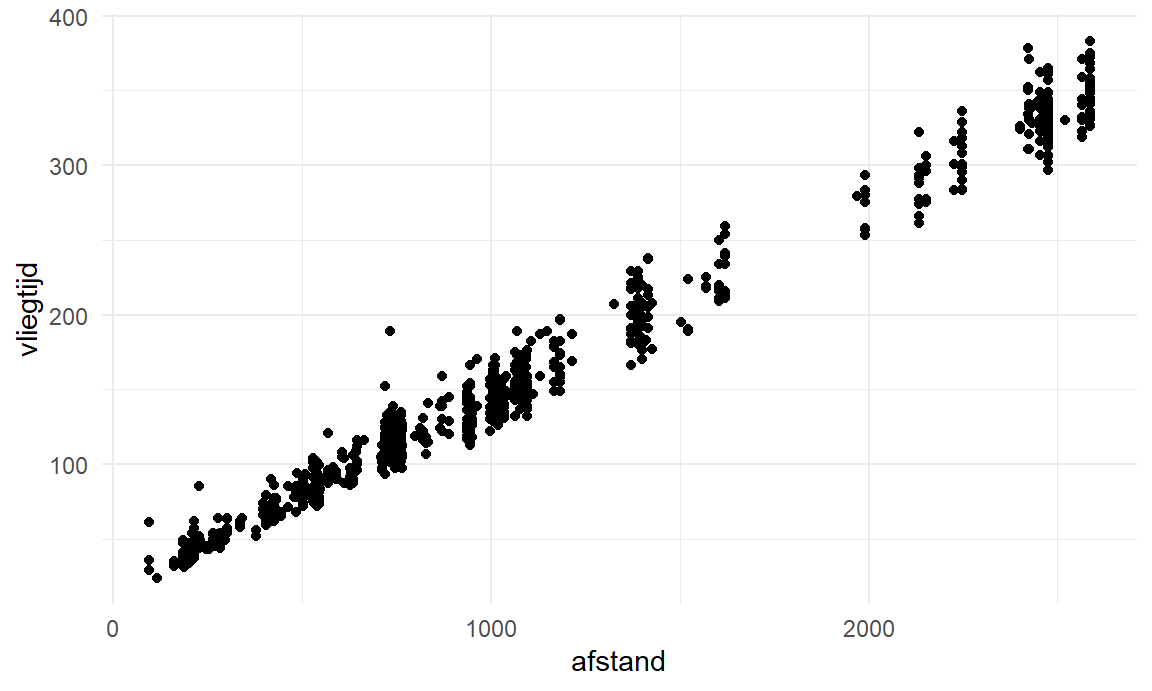
\includegraphics[width=1\linewidth]{textbook_files/figure-latex/213c-1} \caption[Scatterplot]{Scatterplot}\label{fig:213c}
\end{figure}

\begin{itemize}
\tightlist
\item
  Om patronen beter te herkennen kan je een ``trend-lijn'' toevoegen.
\end{itemize}

\begin{figure}
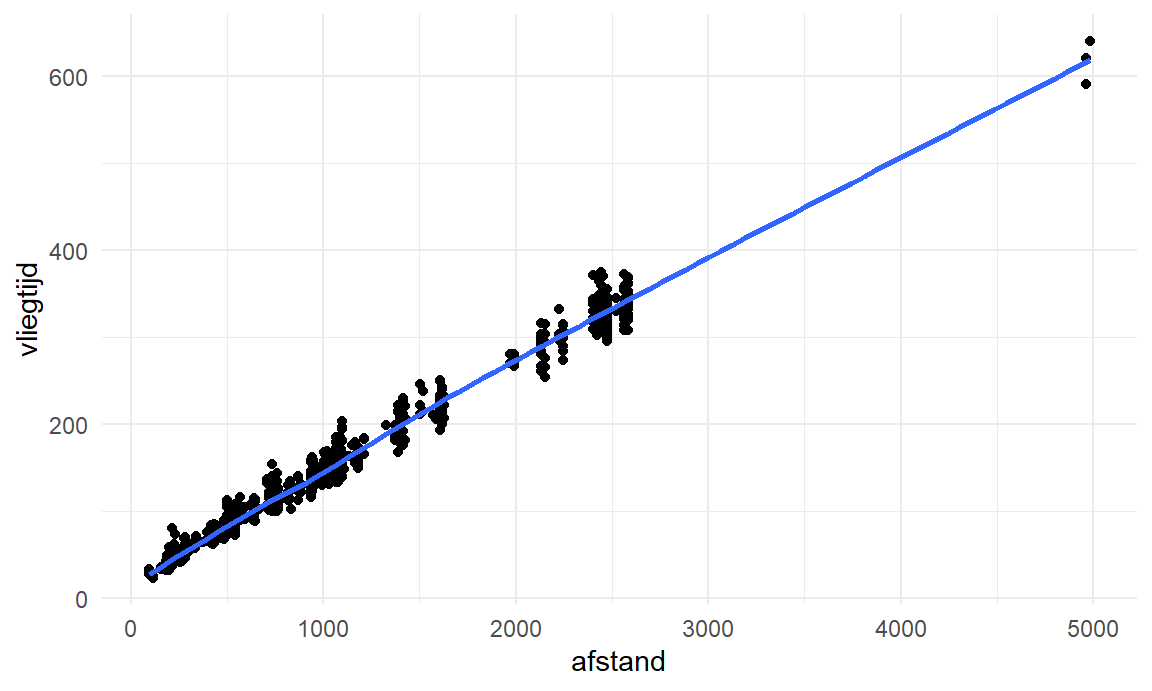
\includegraphics[width=1\linewidth]{textbook_files/figure-latex/2-13d-1} \caption[Scatterplot met trendlijn]{Scatterplot met trendlijn}\label{fig:2-13d}
\end{figure}

\begin{itemize}
\tightlist
\item
  Bij scatterplots is er gevaar voor overplotting
\item
  Mogelijke oplossingen

  \begin{itemize}
  \tightlist
  \item
    2D histogram: verdeel veld op in vierkante bins en tel per bin hoeveel data punten er zijn
  \item
    Hexplot: analoog, maar gebruik zeshoekige bins ipv vierkanten. Voordeel: punten binnen elke zeshoek liggen dichter bij het middelpunt van de bin.
  \end{itemize}
\end{itemize}

\begin{figure}
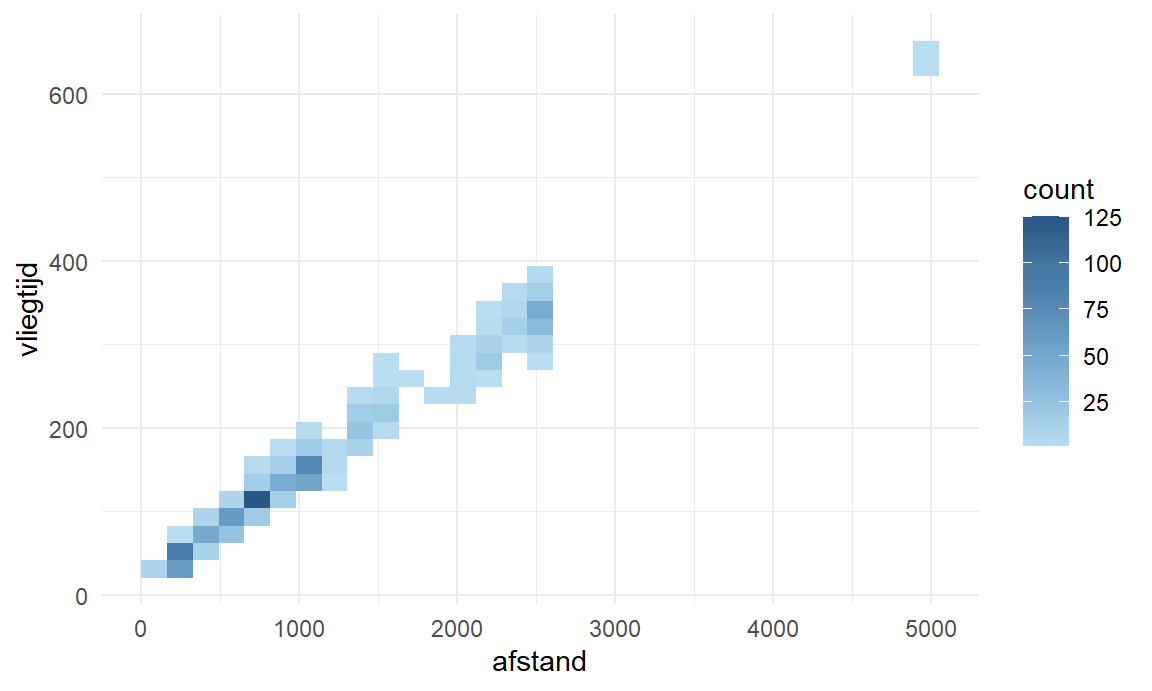
\includegraphics[width=1\linewidth]{textbook_files/figure-latex/unnamed-chunk-10-1} \caption[Scatterplot met trendlijn]{Scatterplot met trendlijn}\label{fig:unnamed-chunk-10}
\end{figure}

\begin{figure}
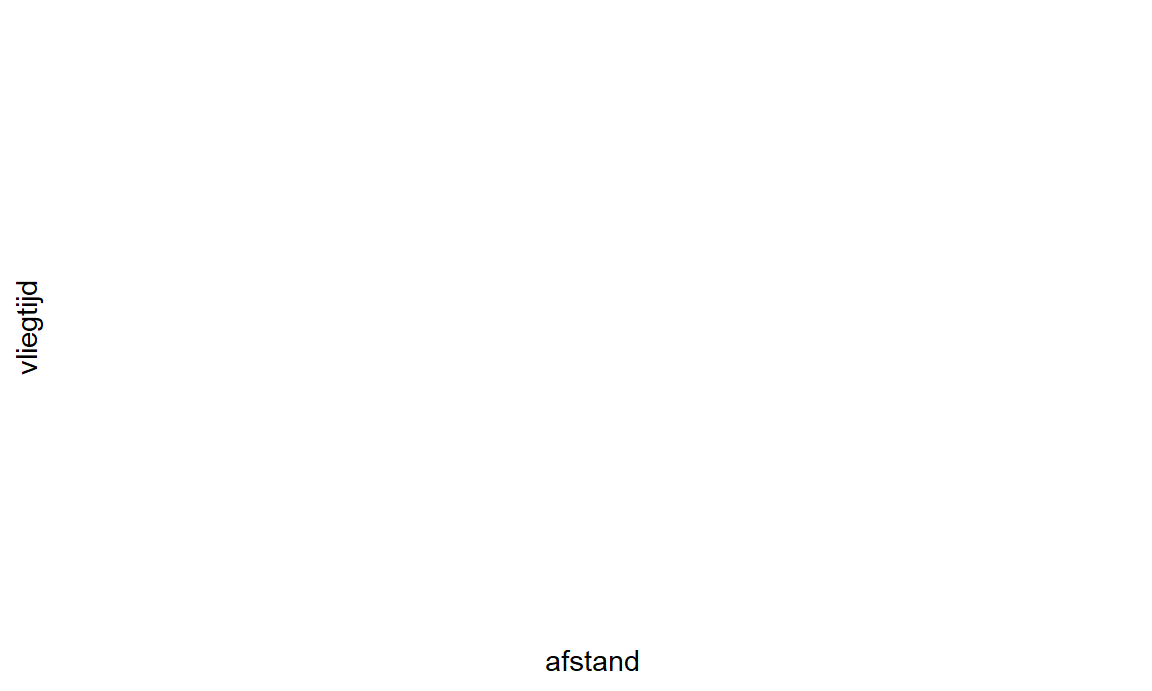
\includegraphics[width=1\linewidth]{textbook_files/figure-latex/unnamed-chunk-11-1} \caption[Hexplot met trendlijn]{Hexplot met trendlijn}\label{fig:unnamed-chunk-11}
\end{figure}

Indien de afhankelijke variabele categorisch is, dan kan je niet rechtstreeks een betekenisvolle plot maken omdat er waarschijnlijk te weinig datapunten zijn voor iedere mogelijke waarde van de onafhankelijke variabele.

\begin{itemize}
\tightlist
\item
  Wat je dan best kan doen, is de onafhankelijke continue variabele categorisch maken door deze in te delen in bins/intervallen. En dan ben je terug in de situatie waarbij de onafhankelijke variabele categorisch is. We komen hierop terug in het hoofdstuk over Data Voorbereiding.
\end{itemize}

\hypertarget{situatie-3-de-onafhankelijke-variabele-is-tijd}{%
\subsection{Situatie 3: De onafhankelijke variabele is tijd}\label{situatie-3-de-onafhankelijke-variabele-is-tijd}}

\begin{itemize}
\tightlist
\item
  Tijd kunnen we zien als continue variabele

  \begin{itemize}
  \tightlist
  \item
    Bijgevolg zelfde grafieken mogelijk als wanneer onafhankelijke variabele continue is

    \begin{itemize}
    \tightlist
    \item
      Tijd + continue afhankelijk -\textgreater{} scatterplot, 2D histograms, hex bins
    \item
      Tijd + categorisch afhankelijk -\textgreater{} probleem: tijd categoriseren (zie verder).
    \end{itemize}
  \end{itemize}
\item
  Wanneer we één enkele variabele voorstellen doorheen de tijd is er per tijdseenheid maar 1 data punt. Hieronder wordt de gemiddelde vertrekvertraging per dag getoond.\\

  \begin{figure}
  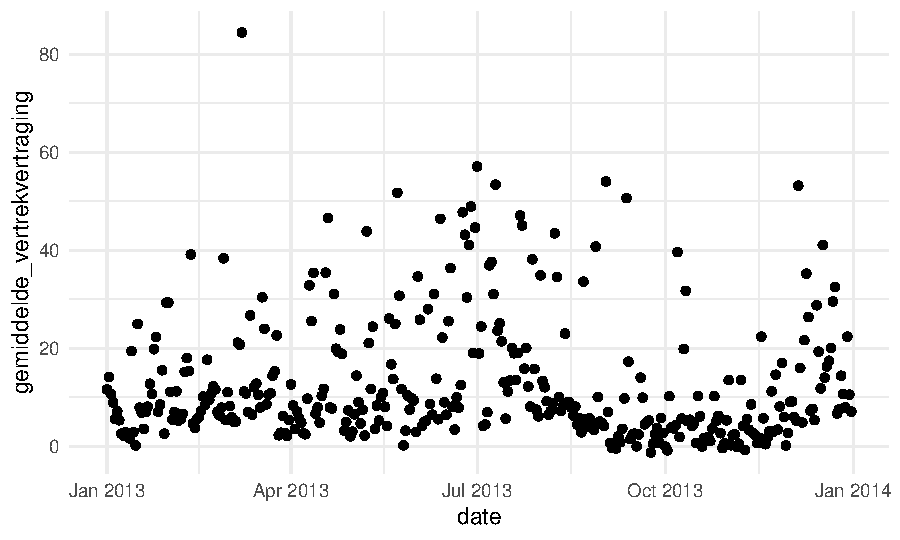
\includegraphics[width=1\linewidth]{textbook_files/figure-latex/unnamed-chunk-12-1} \caption[Puntenwolk met tijd op x-as]{Puntenwolk met tijd op x-as}\label{fig:unnamed-chunk-12}
  \end{figure}
\end{itemize}

In dat geval is het beter om in plaats van punten een lijngrafiek te gebruiken.

\begin{figure}
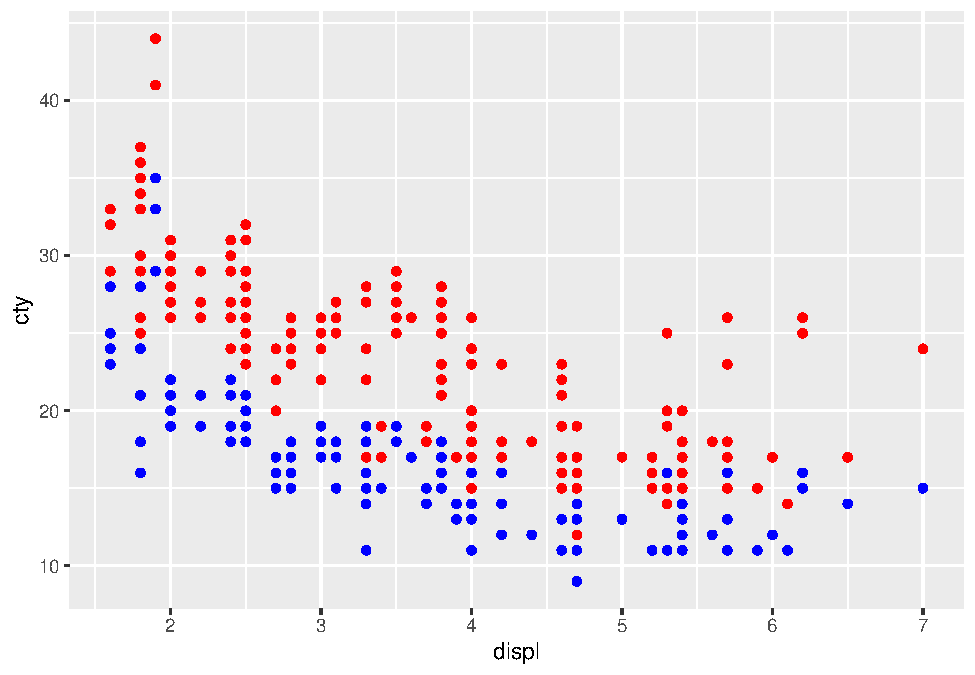
\includegraphics[width=1\linewidth]{textbook_files/figure-latex/unnamed-chunk-13-1} \caption[Lijngrafiek]{Lijngrafiek}\label{fig:unnamed-chunk-13}
\end{figure}

Indien je een beperkt aantal punten hebt (hieronder bijvoorbeeld één maand van de vluchtgegevens) kan je ervoor kiezen om zowel punten als lijnen te tonen. Op die manier is het makkelijker individuele data punten af te lezen.

\begin{figure}
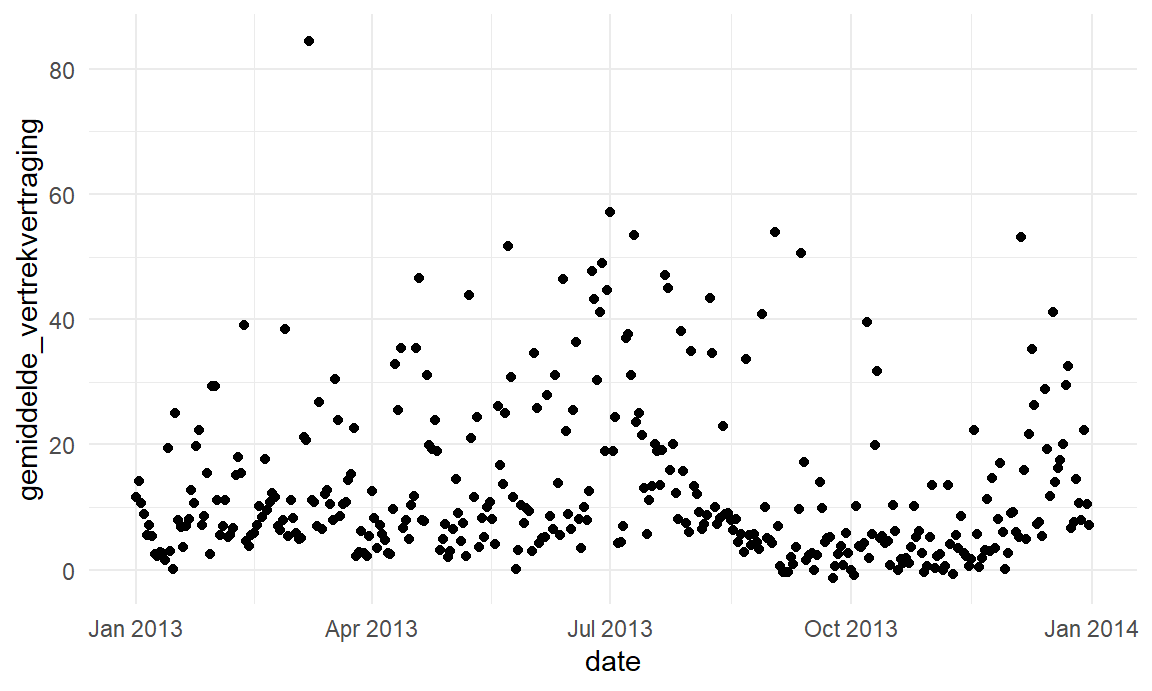
\includegraphics[width=1\linewidth]{textbook_files/figure-latex/unnamed-chunk-14-1} \caption[Lijn grafiek met punten]{Lijn grafiek met punten}\label{fig:unnamed-chunk-14}
\end{figure}

Indien we veel datapunten hebben, wat hier het geval is, kan een lijngrafiek zeer chaotisch worden. We kunnen daarom ervoor kiezen om onze tijd in te delen in categoriëen. Bijvoorbeeld, in plaats van de dagelijkse gemiddelde vertrekvertraging, kunnen we de gemiddelde vertrekvertraging per maand berekenen en tonen.

\begin{figure}
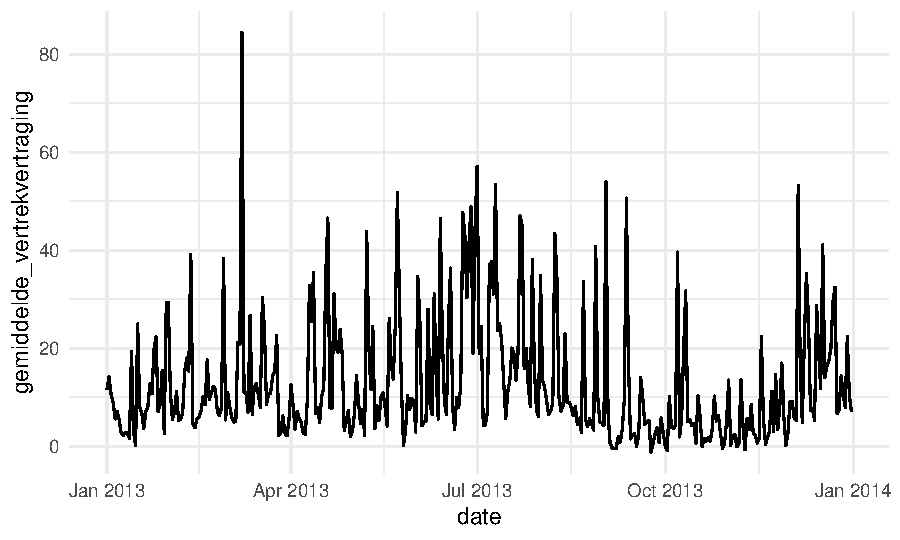
\includegraphics[width=1\linewidth]{textbook_files/figure-latex/unnamed-chunk-15-1} \caption[Lijngrafiek van gemiddelde vertrekvertraging per maand]{Lijngrafiek van gemiddelde vertrekvertraging per maand.}\label{fig:unnamed-chunk-15}
\end{figure}

\begin{itemize}
\tightlist
\item
  Op dit moment verliezen we daardoor wel veel informatie. Maar we kunnen dit nu ook beschouwen als een visualizatie van een categorische variabele (maand) t.o.v. een continue. Waardoor we de technieken voor dit type bivariate visualizaties kunnen toepassen. Bijvoorbeeld boxplots. We zien nu zowel de algemene trend als outliers. In februari was er bijvoorbeeld een dag waar de gemiddelde vertraging ver boven de normale trend lag.
\end{itemize}

\begin{figure}
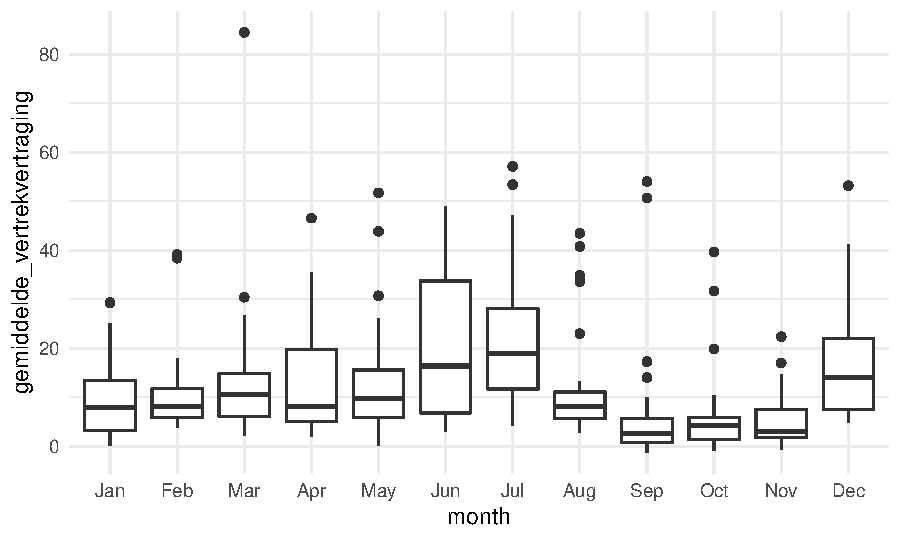
\includegraphics[width=1\linewidth]{textbook_files/figure-latex/unnamed-chunk-16-1} \caption[Boxplots van gemiddelde dagelijske vertrekvertraging voor elke maand]{Boxplots van gemiddelde dagelijske vertrekvertraging voor elke maand.}\label{fig:unnamed-chunk-16}
\end{figure}

\begin{itemize}
\tightlist
\item
  Wanneer we de tijd gecategoriseerd hebben kunnen we ook categorische variabelen weergeven als afhankelijke. Bijvoorbeeld, zijn er verschillen in het aantal vluchten per maatschappij doorheen de tijd. We kunnen hier dezelfde types grafieken als voor bivariate cat+cat visualizaties gebruiken, bijvoorbeeld stacked barcharts.
\end{itemize}

\begin{figure}
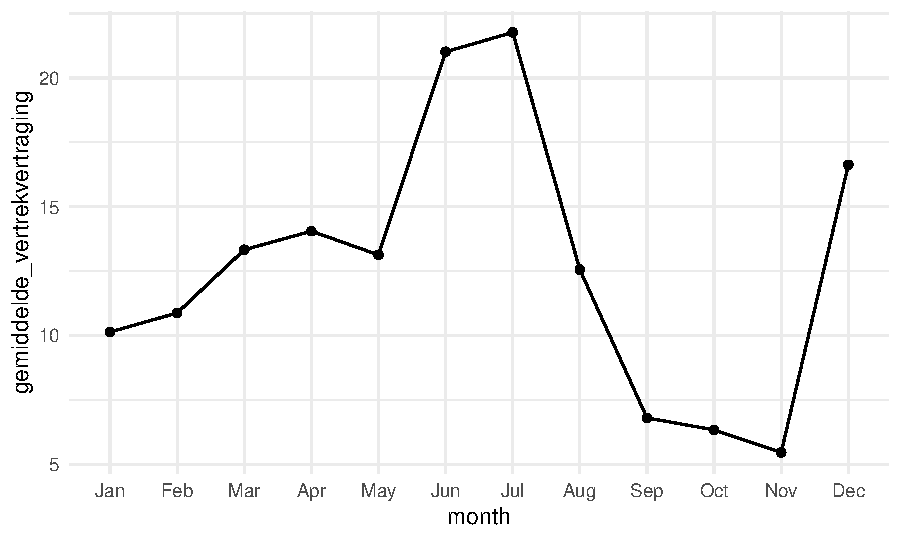
\includegraphics[width=1\linewidth]{textbook_files/figure-latex/unnamed-chunk-17-1} \caption[Verdeling van aantal vluchten over maatschappijen per maand]{Verdeling van aantal vluchten over maatschappijen per maand.}\label{fig:unnamed-chunk-17}
\end{figure}

\begin{itemize}
\tightlist
\item
  We kunnen categorizeren op maand, jaar, etc. Maar ook op tijdspecifiekere kenmerken, zoals bijvoorbeeld de dag van de week
\end{itemize}

\begin{figure}
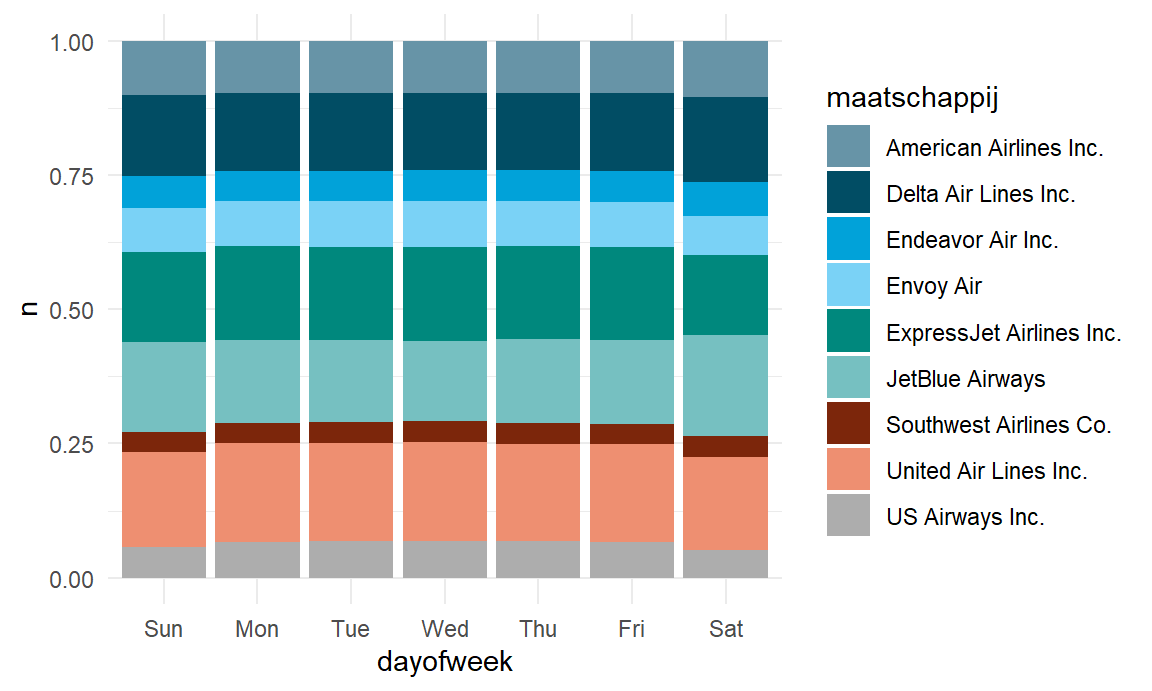
\includegraphics[width=1\linewidth]{textbook_files/figure-latex/unnamed-chunk-18-1} \caption[Verdeling van aantal vluchten over maatschappijen per dag van de week]{Verdeling van aantal vluchten over maatschappijen per dag van de week.}\label{fig:unnamed-chunk-18}
\end{figure}

\begin{itemize}
\tightlist
\item
  Of het uur van de dag
\end{itemize}

\begin{figure}
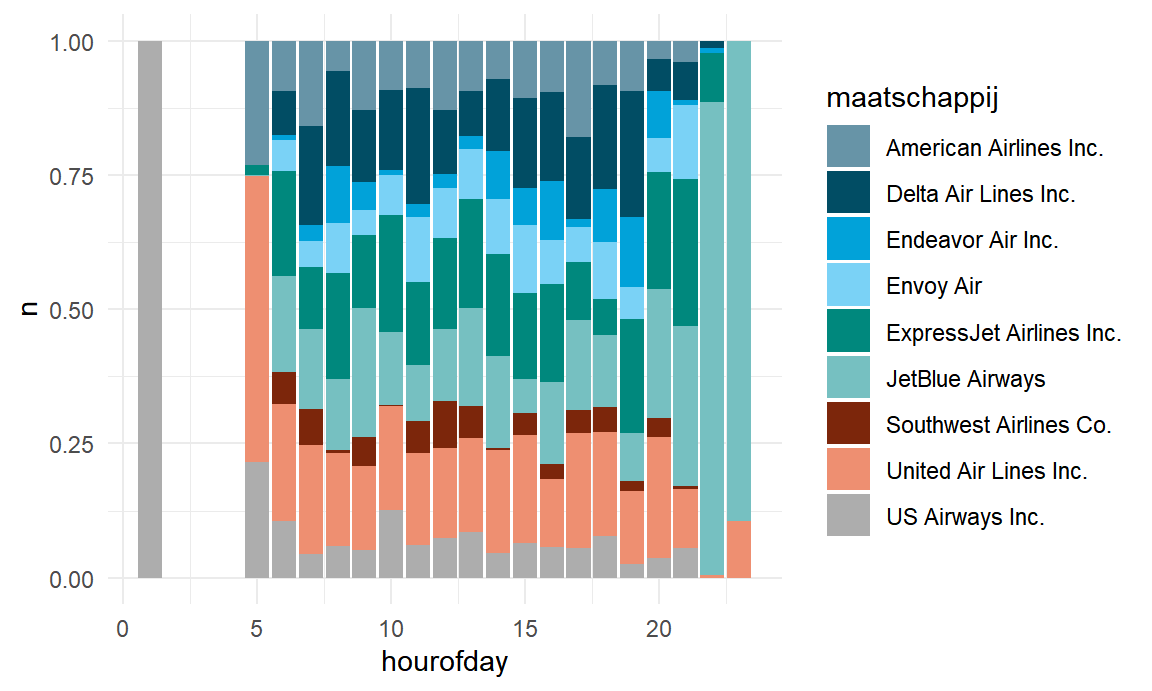
\includegraphics[width=1\linewidth]{textbook_files/figure-latex/unnamed-chunk-19-1} \caption[Verdeling van aantal vluchten over maatschappijen per vertrekuur]{Verdeling van aantal vluchten over maatschappijen per vertrekuur.}\label{fig:unnamed-chunk-19}
\end{figure}

\hypertarget{multivariate-visualisaties-meer-dan-2-variabelen}{%
\section{Multivariate visualisaties (meer dan 2 variabelen)}\label{multivariate-visualisaties-meer-dan-2-variabelen}}

\begin{itemize}
\tightlist
\item
  Datavisualisatie van patronen tussen meer dan 2 variabelen worden snel te complex om te interpreteren.
\item
  Het basisprincipe is wel eenvoudig.

  \begin{itemize}
  \tightlist
  \item
    Je hebt typisch 1 afhankelijke variabele (Y) en een aantal onafhankelijke variabelen (A, B, \ldots).
  \item
    Je visualizeert eerst Y en A (bivariaat)
  \item
    Je voegt dan de volgende variabelen (B, c, \ldots) stap voor stap toe aan de grafiek.

    \begin{itemize}
    \tightlist
    \item
      Door de bivariate grafiek te herhalen in verschillende facetten (een voor elke waarde van B).
    \item
      Door verschillende kleuren te gebruiken voor elke waarde van B
    \end{itemize}
  \end{itemize}
\item
  Bij multivariate visualisaties zijn er afhankelijk van de data types oneidig veel mogelijke grafieken die je kan maken.

  \begin{itemize}
  \tightlist
  \item
    Het is vaak afhankelijk van de data welke grafiek het ``best past''
  \item
    Enkel wanneer de onafhankelijk variabele continu is zijn de keuzes beperkt en ben je vaak genoodzaakt om deze om te zetten naar categoriëen.
  \end{itemize}
\end{itemize}

\hypertarget{voorbeeld-in-welke-mate-hangt-de-vertrek-vertraging-af-van-de-luchthaven-en-de-afstand}{%
\subsection{Voorbeeld: In welke mate hangt de vertrek vertraging af van de luchthaven en de afstand?}\label{voorbeeld-in-welke-mate-hangt-de-vertrek-vertraging-af-van-de-luchthaven-en-de-afstand}}

Stap 1. Vertraging vs.~afstand

\begin{itemize}
\tightlist
\item
  Beide continue: scatterplot
\end{itemize}

\begin{figure}
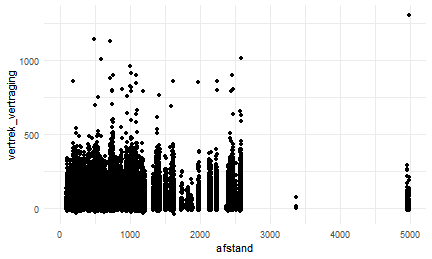
\includegraphics[width=1\linewidth]{textbook_files/figure-latex/labelke-1} \caption[Vertrekvertraging vs afstand]{Vertrekvertraging vs afstand}\label{fig:labelke}
\end{figure}

Stap 2. Voeg invloed van luchthaven toe.

\begin{itemize}
\tightlist
\item
  Optie 1: gebruik kleur om de verschillende luchthavens te differenteren. Een trendlijn kan hier helpen.
\end{itemize}

\begin{figure}
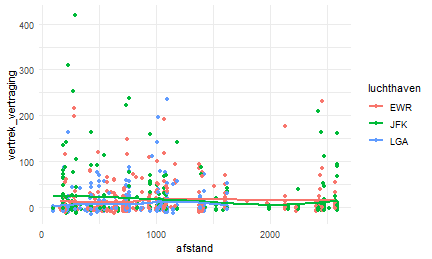
\includegraphics[width=1\linewidth]{textbook_files/figure-latex/labelke2-1} \caption[Vertrekvertraging vs afstand en luchthaven]{Vertrekvertraging vs afstand en luchthaven}\label{fig:labelke2}
\end{figure}

\begin{itemize}
\item
  Geen geweldig resultaat in dit geval.
\item
  Optie 2: Gebruik facetten voor de verschillende luchthavens.
\end{itemize}

\begin{figure*}
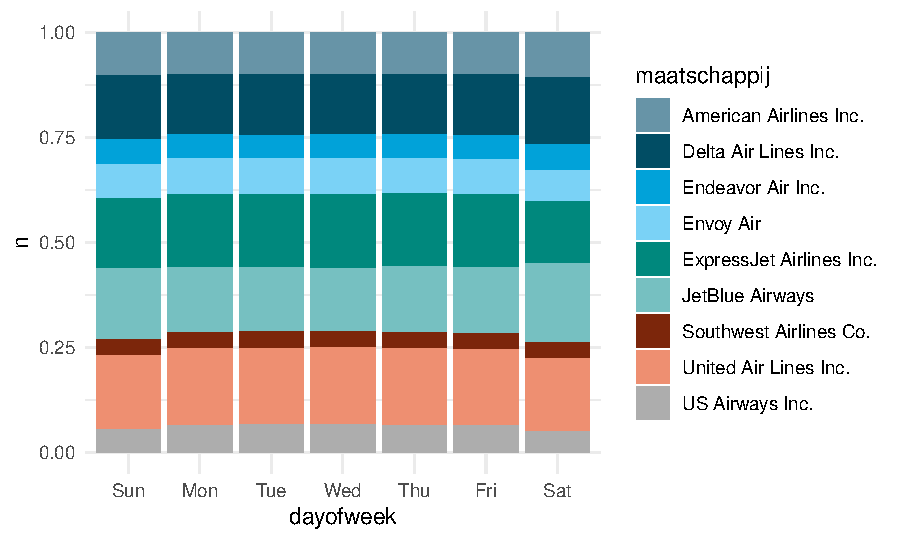
\includegraphics[width=1\linewidth]{textbook_files/figure-latex/unnamed-chunk-20-1} \caption[Vertrekvertraging vs afstand en luchthaven]{Vertrekvertraging vs afstand en luchthaven}\label{fig:unnamed-chunk-20}
\end{figure*}

\begin{itemize}
\tightlist
\item
  Optie 3: Facets, maar gebruik hex bins
\end{itemize}

\begin{figure*}
\includegraphics[width=1\linewidth]{textbook_files/figure-latex/unnamed-chunk-21-1} \caption[Vertrekvertraging vs afstand en luchthaven, hexbins]{Vertrekvertraging vs afstand en luchthaven, hexbins}\label{fig:unnamed-chunk-21}
\end{figure*}

\hypertarget{voorbeeld-multivariaat-tijd}{%
\subsection{Voorbeeld: multivariaat tijd}\label{voorbeeld-multivariaat-tijd}}

\hypertarget{situatie-1-variabelen-hebben-dezelfde-eenheid.}{%
\subsubsection{Situatie 1: Variabelen hebben dezelfde eenheid.}\label{situatie-1-variabelen-hebben-dezelfde-eenheid.}}

Voorbeeld: vertrekvertraging en aankomstvertraging. Je kan lijngrafieken tekenen met meerdere lijnen op hetzelfde assenstelsel.

\begin{figure}
\includegraphics[width=1\linewidth]{textbook_files/figure-latex/unnamed-chunk-22-1} \caption[Evolutie van 2 variabelen over tijd in één grafiek (zelfde meeteenheid)]{Evolutie van 2 variabelen over tijd in één grafiek (zelfde meeteenheid)}\label{fig:unnamed-chunk-22}
\end{figure}

\begin{itemize}
\tightlist
\item
  Of je kan er voor kiezen elke lijn in een afzonderlijk paneel te tonen
\end{itemize}

\begin{figure}
\includegraphics[width=1\linewidth]{textbook_files/figure-latex/unnamed-chunk-23-1} \caption[Evolutie van 2 variabelen over tijd in afzondelijke panels]{Evolutie van 2 variabelen over tijd in afzondelijke panels.}\label{fig:unnamed-chunk-23}
\end{figure}

\hypertarget{situatie-2-variabelen-hebben-niet-dezelfde-eenheid}{%
\subsubsection{Situatie 2: Variabelen hebben niet dezelfde eenheid}\label{situatie-2-variabelen-hebben-niet-dezelfde-eenheid}}

Voorbeeld: de gemiddelde levensverwachting en gdp per capita doorheen de tijd. In dit geval ben je genoodzaakt 2 panelen te gebruiken.

\begin{figure}
\includegraphics[width=1\linewidth]{textbook_files/figure-latex/unnamed-chunk-24-1} \caption[Evolutie van 2 variabelen met andere eenheden in afzonderlijke panels]{Evolutie van 2 variabelen met andere eenheden in afzonderlijke panels.}\label{fig:unnamed-chunk-24}
\end{figure}

Optie 2: Maak een connected scatterplot. Toon een punt voor elke meting, waarbij x en y elk een variabele voorstellen. Verbindt dat elk punt in chronologische volgorde.

\begin{figure}
\includegraphics[width=1\linewidth]{textbook_files/figure-latex/unnamed-chunk-25-1} \caption[Evolutie van 2 variabelen (levensverwachting en inkomen per capita) aan de hand van connected scatterplot]{Evolutie van 2 variabelen (levensverwachting en inkomen per capita) aan de hand van connected scatterplot.}\label{fig:unnamed-chunk-25}
\end{figure}

Variant, per continent:

\begin{figure}
\includegraphics[width=1\linewidth]{textbook_files/figure-latex/unnamed-chunk-26-1} \caption[Evolutie van 2 variabelen aan de hand van connected scatterplot - verschillende groepen]{Evolutie van 2 variabelen aan de hand van connected scatterplot - verschillende groepen.}\label{fig:unnamed-chunk-26}
\end{figure}

\hypertarget{visualisaties-voor-communicatie}{%
\section{Visualisaties voor communicatie}\label{visualisaties-voor-communicatie}}

Wanneer uiteindelijk beslist om een visualizatie te gebruiken om te communiceren, zorg ervoor dat

\begin{itemize}
\tightlist
\item
  de grafiek leesbaar is
\item
  je kleur enkel gebruikt waar nodig.
\item
  je correcte as-labels gebruikt
\item
  je geen theme gebruikt dat te druk/overheersend is
\item
  je een gepaste titel voorziet.
\end{itemize}

\hypertarget{voorbeeld-voor-goed-voor-exploratie}{%
\subsection{Voorbeeld: voor \textasciitilde{} goed voor exploratie}\label{voorbeeld-voor-goed-voor-exploratie}}

\includegraphics[width=1\linewidth]{textbook_files/figure-latex/unnamed-chunk-27-1}

\hypertarget{voorbeeld-na-goed-voor-communicatie}{%
\subsection{Voorbeeld: na \textasciitilde{} goed voor communicatie}\label{voorbeeld-na-goed-voor-communicatie}}

\includegraphics[width=1\linewidth]{textbook_files/figure-latex/unnamed-chunk-28-1}

Merk op: ver van alle grafieken getoond in dit hoofdstuk zijn goed voor communicatie zonder aanpassingen.

\hypertarget{how-charts-lie}{%
\section{How charts lie}\label{how-charts-lie}}

\hypertarget{causaliteit-vs-correlatie}{%
\subsection{Causaliteit vs correlatie}\label{causaliteit-vs-correlatie}}

\begin{itemize}
\tightlist
\item
  Van zodra er twee (or meer) variabelen zijn, gaan we op zoek naar patronen in relaties tussen de variabelen.
\item
  Het is belangrijk en essentieel te beseffen dat mensen een automatische reflex hebben om te denken in termen van oorzaak-gevolg als we kijken naar relaties tussen twee variabelen.

  \begin{itemize}
  \tightlist
  \item
    Het is echter niet omdat er een duidelijke relatie bestaat tussen twee variabelen (correlatie), dat hier sprake is van een oorzaak-gevolg verband (causaliteit).
  \item
    Bijvoorbeeld: Indien in de zomer de verkoop van paraplu's sterk stijgt, dan zal de graanopbrengst in het najaar dalen. Dit betekent niet dat de verkoop van paraplu's een impact heeft op de graanopbrengst. Wat hier waarschijnlijk gebeurt, is dat door hevige regenval in de zomermaanden, de verkoop van paraplu's is toegenomen en de graanoogst tegenvalt.

    \begin{itemize}
    \tightlist
    \item
      Soms is het intuïtief zeer onwaarschijnlijk dat de waargenomen correlatie causaliteit impliceert. Kijk hiervoor maar eens naar de voorbeelden op \url{http://www.tylervigen.com/spurious-correlations}
    \item
      Wanneer het echter plausibel is dat de waargenomen correlatie causaliteit voorstelt, is het belangrijk dat we tegen onze natuurlijke reflex in gaan en niet in termen van oorzaak-gevolg denken.
    \item
      Het aantonen van causaliteit is nooit mogelijk met descriptieve en exploratieve data analyse!
    \end{itemize}
  \end{itemize}
\end{itemize}

\hypertarget{referenties-1}{%
\section{Referenties}\label{referenties-1}}

\begin{itemize}
\tightlist
\item
  \href{https://informationisbeautiful.net/}{Information is Beautiful}
\item
  \href{https://serialmentor.com/dataviz/}{Fundamentals of Data Vizualization}
\item
  \href{https://www.r-graph-gallery.com/}{R Graph Gallery}
\item
  \href{https://www.data-to-viz.com/}{Data to viz}
\item
  \href{https://www.tylervigen.com/spurious-correlations}{Spurrious correlations}
\item
  \href{https://edition.cnn.com/2020/01/17/politics/donald-trump-2016-map-county-by-county/index.html}{Misleading election map}
\end{itemize}

\hypertarget{tutorial-data-visualisatie}{%
\chapter{{[}Tutorial{]} Data visualisatie}\label{tutorial-data-visualisatie}}

\hypertarget{voor-je-begint}{%
\section{Voor je begint}\label{voor-je-begint}}

Voordat je met deze zelfstudie begint, moet je eerst het pakket \texttt{ggplot2} installeren, als je dat nog niet gedaan hebt. Je kunt dit doen met de volgende regel code:

\begin{Shaded}
\begin{Highlighting}[]
\FunctionTok{install.packages}\NormalTok{(}\StringTok{"ggplot2"}\NormalTok{)}
\end{Highlighting}
\end{Shaded}

In ieder geval, moet je het pakket in je sessie laden.

\begin{Shaded}
\begin{Highlighting}[]
\FunctionTok{library}\NormalTok{(ggplot2)}
\end{Highlighting}
\end{Shaded}

Je hebt ook twee datasets nodig, \texttt{movies} en \texttt{diamonds}. Beide worden als .RDS bestand bij deze tutorial geleverd.

\begin{Shaded}
\begin{Highlighting}[]
\NormalTok{movies }\OtherTok{\textless{}{-}} \FunctionTok{readRDS}\NormalTok{(}\StringTok{"movies.RDS"}\NormalTok{)}
\NormalTok{diamonds }\OtherTok{\textless{}{-}} \FunctionTok{readRDS}\NormalTok{(}\StringTok{"diamonds.RDS"}\NormalTok{)}
\end{Highlighting}
\end{Shaded}

\hypertarget{introductie}{%
\section{Introductie}\label{introductie}}

Het maken van een plot met ggplot2 begint met de \texttt{ggplot()} functie. De ggplot functie heeft twee belangrijke argumenten

\begin{itemize}
\tightlist
\item
  \textbf{data}: dit definieert de dataset die voor de plot moet worden gebruikt. Dit moet een data.frame zijn.
\item
  \textbf{mapping}: de mapping zal bepalen hoe de variabelen worden \emph{mapped} op de esthetica\footnote{De \emph{aesthetics} van een ggplot-grafiek zijn de visuals die we in de grafiek zien: positie, kleur, vorm, grootte, linetype, enz.} van de plot, zoals verderop zal worden uitgelegd. Deze mapping moet altijd worden gemaakt met de \texttt{aes()} functie .
\end{itemize}

We willen bijvoorbeeld een scatterplot maken van de films, waarbij we de x-as gebruiken voor hun budget en de y-as voor hun waardering. We roepen ggplot dan als volgt aan:

\begin{Shaded}
\begin{Highlighting}[]
\FunctionTok{ggplot}\NormalTok{(}\AttributeTok{data =}\NormalTok{ movies, }\AttributeTok{mapping =} \FunctionTok{aes}\NormalTok{(}\AttributeTok{x =}\NormalTok{ budget, }\AttributeTok{y =}\NormalTok{ rating))}
\end{Highlighting}
\end{Shaded}

\includegraphics[width=1\linewidth]{textbook_files/figure-latex/unnamed-chunk-34-1}

Zoals je ziet, creëert deze regel code een plot met de assen zoals gedefinieerd. Er worden echter geen gegevens gevisualiseerd. De reden hiervoor is dat ggplot nog niet weet hoe we het willen visualiseren. We moeten wat genoemd wordt \emph{een geometrische layer} toevoegen. Om een scatterplot te maken, die uit \emph{punten} bestaat, voegen we \texttt{geom\_point} aan de plot toe.

\begin{Shaded}
\begin{Highlighting}[]
\FunctionTok{ggplot}\NormalTok{(}\AttributeTok{data =}\NormalTok{ movies, }\AttributeTok{mapping =} \FunctionTok{aes}\NormalTok{(}\AttributeTok{x =}\NormalTok{ budget, }\AttributeTok{y =}\NormalTok{ rating)) }\SpecialCharTok{+}
  \FunctionTok{geom\_point}\NormalTok{()}
\end{Highlighting}
\end{Shaded}

\includegraphics[width=1\linewidth]{textbook_files/figure-latex/unnamed-chunk-35-1}

Dit lijkt er al meer op. Merk op dat de geometrische laag aan de plot is toegevoegd door gebruik te maken van het \texttt{+} symbool. Op deze manier kunnen meerdere lagen aan dezelfde plot worden toegevoegd, evenals titels, labels, en configuraties van de lay-out, zoals we verderop zullen zien.

Merk op dat we de mapping van de \emph{aesthetics} ook in de geometrische laag zelf kunnen plaatsen. Dit maakt onze code voorlopig iets leesbaarder, omdat we de geometrische layer en de mapping ervan op dezelfde regel plaatsen.

\begin{Shaded}
\begin{Highlighting}[]
\FunctionTok{ggplot}\NormalTok{(}\AttributeTok{data =}\NormalTok{ movies) }\SpecialCharTok{+}
  \FunctionTok{geom\_point}\NormalTok{(}\AttributeTok{mapping =} \FunctionTok{aes}\NormalTok{(}\AttributeTok{x =}\NormalTok{ budget, }\AttributeTok{y =}\NormalTok{ rating))}
\end{Highlighting}
\end{Shaded}

\includegraphics[width=1\linewidth]{textbook_files/figure-latex/unnamed-chunk-36-1}

We hebben nu onze allereerste plot gemaakt! In de volgende secties zullen we leren hoe we verschillende geom-layers en \emph{aesthetics} kunnen gebruiken en hoe we de lay-out van onze grafieken kunnen verbeteren.

\hypertarget{verschillende-geometrics}{%
\section{Verschillende geometrics}\label{verschillende-geometrics}}

Naast \texttt{geom\_point} bestaan er nog veel meer verschillende geometrieën om gegevens in ggplot te plotten. Je kunt ze bekijken door `geom\_' in het console in te typen en door de auto-complete-lijst te navigeren. Elk van de geom-layers komt met zijn eigen specifieke set van \emph{aesthetics} die in kaart gebracht kan (en soms moet) worden. In deze tutorial zullen we ons vooral richten op de volgende geometrische lagen:

\begin{itemize}
\tightlist
\item
  geom\_point
\item
  geom\_histogram
\item
  geom\_boxplot
\item
  geom\_violin
\item
  geom\_bar
\item
  geom\_col
\end{itemize}

\hypertarget{geom_point}{%
\subsection{geom\_point}\label{geom_point}}

We hebben \texttt{geom\_point} al gebruikt om onze eerste grafiek te maken, waarbij we twee variabelen in kaart brachten op de esthetica \emph{x} en \emph{y}. Er zijn echter nog enkele andere aesthetics's die met deze laag kunnen worden ingesteld. Laten we ze eens in meer detail bekijken.

\begin{itemize}
\tightlist
\item
  \textbf{x}: dit bepaalt de positie van de punten langs de x-as
\item
  \textbf{y}: hiermee bepaal je de positie van de punten langs de y-as
\item
  \textbf{color}: hiermee bepaal je de kleur van de punten
\item
  \textbf{shape}: hiermee bepaal je het type punten dat uitgezet moet worden\footnote{\includegraphics{images/points-symbols.png} Naast een normaal punt, kunnen veel verschillende vormen worden uitgezet in ggplot. Deze figuur toont de belangrijkste. De vormen kunnen worden gebruikt door de aesthetic `shape' in te stellen op het bijbehorende nummer.}
\item
  \textbf{fill}: hiermee bepaal je hoe de punten gevuld worden (voor vormen 21-25)
\item
  \textbf{size}: hiermee bepaal je de grootte van de punten
\item
  \textbf{stroke}: hiermee bepaal je de breedte van de rand
\item
  \textbf{alpha}: hiermee bepaal je de mate van doorzichtigheid
\end{itemize}

De onderstaande grafiek bijvoorbeeld toont zwarte driehoeken, gevuld met rood, met een grootte van 2. Merk op dat de positie van de driehoeken precies dezelfde is als de positie van de punten in de vorige grafiek.

\begin{Shaded}
\begin{Highlighting}[]
\FunctionTok{ggplot}\NormalTok{(}\AttributeTok{data =}\NormalTok{ movies) }\SpecialCharTok{+}
  \FunctionTok{geom\_point}\NormalTok{(}
    \AttributeTok{mapping =} \FunctionTok{aes}\NormalTok{(}\AttributeTok{x =}\NormalTok{ budget, }\AttributeTok{y =}\NormalTok{ rating),}
    \AttributeTok{shape =} \DecValTok{24}\NormalTok{,}
    \AttributeTok{fill =} \StringTok{"red"}\NormalTok{,}
    \AttributeTok{color =} \StringTok{"black"}\NormalTok{,}
    \AttributeTok{size =} \DecValTok{2}
\NormalTok{  )}
\end{Highlighting}
\end{Shaded}

\includegraphics[width=1\linewidth]{textbook_files/figure-latex/unnamed-chunk-37-1}

Maar wacht, er is hier iets belangrijks aan de hand! Terwijl de x- en y-aesthetics binnen de aes-mapping werden gedefinieerd, werden de andere aesthetic erbuiten gedefinieerd. Waarom is dat?

In feite kunnen aesthetics op twee verschillende manieren worden ingesteld:

\begin{enumerate}
\def\labelenumi{\arabic{enumi}.}
\tightlist
\item
  Ze kunnen worden \emph{mapped} naar een variabele in de dataset.
\item
  Ze kunnen worden ingesteld op één vaste waarde.
\end{enumerate}

In ons voorbeeld worden x en y gekoppeld aan twee variabelen in de gegevens, nl. budget en rating, terwijl de andere aesthetics, vorm, fill, color en size, worden ingesteld op vaste waarden. Hoewel sommige aesthetics typisch altijd gemapt worden, zoals x- en y-posities, kunnen sommige andere zowel een vaste waarde als een gemapte variabele zijn. Bijvoorbeeld, wat gebeurt er als we de kleur van punten toewijzen aan een variabele, zeg de variabele Action.

\begin{Shaded}
\begin{Highlighting}[]
\FunctionTok{ggplot}\NormalTok{(}\AttributeTok{data =}\NormalTok{ movies) }\SpecialCharTok{+}
  \FunctionTok{geom\_point}\NormalTok{(}\AttributeTok{mapping =} \FunctionTok{aes}\NormalTok{(}
    \AttributeTok{x =}\NormalTok{ budget,}
    \AttributeTok{y =}\NormalTok{ rating,}
    \AttributeTok{color =}\NormalTok{ Action}
\NormalTok{  ))}
\end{Highlighting}
\end{Shaded}

\includegraphics[width=1\linewidth]{textbook_files/figure-latex/unnamed-chunk-38-1}

We zien dat de punten nu gekleurd zijn met betrekking tot de waarde in de variabele Action. Action films krijgen een groene kleur, terwijl andere films een rode kleur krijgen, wat we kunnen zien in de legende die verscheen.

Ook de andere vaste aesthetics kunnen worden gebruikt in een mapping. Het volgende voorbeeld gebruikt de variabele Animatie voor de shape.

\begin{Shaded}
\begin{Highlighting}[]
\FunctionTok{ggplot}\NormalTok{(}\AttributeTok{data =}\NormalTok{ movies) }\SpecialCharTok{+}
  \FunctionTok{geom\_point}\NormalTok{(}\AttributeTok{mapping =} \FunctionTok{aes}\NormalTok{(}
    \AttributeTok{x =}\NormalTok{ budget,}
    \AttributeTok{y =}\NormalTok{ rating,}
    \AttributeTok{color =}\NormalTok{ Action,}
    \AttributeTok{shape =}\NormalTok{ Animation}
\NormalTok{  ))}
\end{Highlighting}
\end{Shaded}

\includegraphics[width=1\linewidth]{textbook_files/figure-latex/unnamed-chunk-39-1}

Geweldig! We begrijpen nu volledig de geom\_point laag, en de werking van de aesthetics-mapping. Nu is het tijd om enkele andere geometrische layers te bekijken. We beginnen met histogrammen.

\hypertarget{geom_histogram}{%
\subsection{geom\_histogram}\label{geom_histogram}}

De \emph{geom\_histogram} layer kan worden gebruikt om een histogram uit te zetten. Zoals je al zou moeten weten, geeft een histogram de verdeling van \textbf{een} continue variabele weer. Bijgevolg moet er alleen een x-aesthetic worden ingesteld, en geen y-aesthetic. De volledige lijst van aesthetic's is als volgt:

\begin{itemize}
\tightlist
\item
  \textbf{x}: dit bepaalt de variabele die gebruikt moet worden
\item
  \textbf{color}: hiermee bepaal je de kleur van de randen
\item
  \textbf{fill}: hiermee bepaal je met welke kleur het histogram gevuld wordt
\item
  \textbf{size}: hiermee bepaal je de grootte van de rand
\item
  \textbf{linetype}: hiermee bepaal je het type van de rand \footnote{\includegraphics{images/line_types.png} Naast een normale lijn, kunnen verschillende andere linetypes geplot worden in ggplot. De types kunnen worden gebruikt door de aesthetic `linetype' in te stellen op het bijbehorende nummer, of op de naam van het type. Net al shape voor geom\_point.}
\item
  \textbf{alpha}: hiermee bepaal je de mate van doorzichtigheid
\item
  \textbf{weight}: hiermee bepaal je hoe de waarnemingen gewogen moeten worden. Standaard wordt elke waarneming als één gewogen.
\end{itemize}

Gebruik makend van onze kennis over het gebruik van aesthetics van voorheen, is het nu heel eenvoudig om een histogram te maken. Laten we een histogram maken voor de beoordeling van films. We geven het een zwarte rand met een witte vulling. Klaar om te proberen?

\begin{Shaded}
\begin{Highlighting}[]
\FunctionTok{ggplot}\NormalTok{(movies) }\SpecialCharTok{+}
  \FunctionTok{geom\_histogram}\NormalTok{(}\FunctionTok{aes}\NormalTok{(rating), }\AttributeTok{color =} \StringTok{"black"}\NormalTok{, }\AttributeTok{fill =} \StringTok{"white"}\NormalTok{)}
\end{Highlighting}
\end{Shaded}

\includegraphics[width=1\linewidth]{textbook_files/figure-latex/unnamed-chunk-40-1}

Merk op dat verschillende dingen werden weggelaten in deze twee lijnen van codes. In het bijzonder de argumentnaam \emph{data} in ggplot, \emph{mapping} in geom\_histogram en \emph{x} in aes. Aangezien we weten dat dit de eerste argumenten van deze functies zijn, kunnen we ze veilig weglaten, zolang we de juiste volgorde van argumenten aanhouden. We kunnen echter \emph{color} en \emph{fill} niet weglaten, omdat dit niet het tweede en derde argument van geom\_histogram zijn. Speel in geval van twijfel op veilig en schrijf de juiste argumentnamen.

Dat is echter niet het enige dat hier opvallend is. Inderdaad, er verschijnt een waarschuwing: \texttt{stat\_bin()} using \texttt{bins\ =\ 30}. Pick better value with \texttt{binwidth}. Deze waarschuwing herinnert ons aan het feit dat een standaard waarde voor het aantal bins is gekozen door geom\_histogram, die waarschijnlijk niet geschikt is voor onze grafiek. We kunnen de binbreedte veranderen door deze als argument toe te voegen aan de aanroep geom\_histogram.

\begin{Shaded}
\begin{Highlighting}[]
\FunctionTok{ggplot}\NormalTok{(movies) }\SpecialCharTok{+}
  \FunctionTok{geom\_histogram}\NormalTok{(}\FunctionTok{aes}\NormalTok{(rating), }\AttributeTok{color =} \StringTok{"black"}\NormalTok{, }\AttributeTok{fill =} \StringTok{"white"}\NormalTok{, }\AttributeTok{binwidth =} \FloatTok{0.5}\NormalTok{)}
\end{Highlighting}
\end{Shaded}

\includegraphics[width=1\linewidth]{textbook_files/figure-latex/unnamed-chunk-41-1}

Vaak heeft de binbreedte een belangrijke invloed op hoe het verkregen histogram eruit ziet. Zorgvuldig configureren van dit argument door te experimenteren met verschillende waarden is daarom belangrijk.

In de laatste plot hebben we een vaste kleur gebruikt voor het vullen van de balken van het histogram. Maar zoals we ondertussen al weten, kunnen we die ook toewijzen aan een variabele in de gegevens. Laten we de variabele \emph{Action} nog een keer gebruiken.

\begin{Shaded}
\begin{Highlighting}[]
\FunctionTok{ggplot}\NormalTok{(movies) }\SpecialCharTok{+}
  \FunctionTok{geom\_histogram}\NormalTok{(}\FunctionTok{aes}\NormalTok{(rating, }\AttributeTok{fill =}\NormalTok{ Action), }\AttributeTok{color =} \StringTok{"black"}\NormalTok{, }\AttributeTok{binwidth =} \FloatTok{0.5}\NormalTok{)}
\end{Highlighting}
\end{Shaded}

\includegraphics[width=1\linewidth]{textbook_files/figure-latex/unnamed-chunk-42-1}

Merk op hoe we het fill-argument binnen de \texttt{aes} functie hebben geplaatst. Nu is elke staaf gevuld met twee kleuren: een deel voor actie-films, en de rest voor andere films. Hoewel het niet erg duidelijk is in deze grafiek, lijkt het erop dat het centrum van het histogram voor actiefilms iets meer naar links ligt.

Merk op hoe de notatie verandert bij de overgang naar de aes-mapping: variabelennamen worden altijd zonder aanhalingstekens gebruikt, terwijl vaste aesthetics (kleuren, vormen, linetypes) met aanhalingstekens worden gebruikt (behalve voor getallen). Het is belangrijk om dit niet door elkaar te halen! Nooit aanhalingstekens rond namen van variabelen!

Standaard zijn de histogrammen voor de verschillende \emph{fills} \emph{stacked}, d.w.z. boven elkaar geplaatst. We kunnen echter het \emph{position} argument van geom\_histogram gebruiken om de staven naast elkaar te plaatsen, of \emph{dodged}.

\begin{Shaded}
\begin{Highlighting}[]
\FunctionTok{ggplot}\NormalTok{(movies) }\SpecialCharTok{+}
  \FunctionTok{geom\_histogram}\NormalTok{(}\FunctionTok{aes}\NormalTok{(rating, }\AttributeTok{fill =}\NormalTok{ Action),}
    \AttributeTok{color =} \StringTok{"black"}\NormalTok{, }\AttributeTok{binwidth =} \FloatTok{0.5}\NormalTok{, }\AttributeTok{position =} \StringTok{"dodge"}
\NormalTok{  )}
\end{Highlighting}
\end{Shaded}

\includegraphics[width=1\linewidth]{textbook_files/figure-latex/unnamed-chunk-43-1}

Met position = ``dodge'' worden de balken voor actiefilms en niet-actiefilms naast elkaar geplaatst, in plaats van boven elkaar. We kunnen teruggaan naar de oorspronkelijke grafiek door position = ``stack'' te gebruiken, of door dit argument weg te laten. Later zullen we zien hoe we beter met dergelijke zaken kunnen omgaan door gebruik te maken van rasters van verschillende plots, of zogenaamde \emph{facets}.

Alles goed tot nu toe? Laten we eens kijken naar een andere manier om de verdeling van continue variabelen te visualiseren, namelijk de boxplot.

\hypertarget{geom_boxplot}{%
\subsection{geom\_boxplot}\label{geom_boxplot}}

Een boxplot plaatst de waarden van de variabele op de y-as. Dus, als we een boxplot willen maken voor ratings, moeten we \texttt{aes(y\ =\ ratings)} gebruiken. Er is hier echter iets tricky aan de hand\ldots{} De aesthetics voor geom\_boxplot is de volgende

\begin{itemize}
\tightlist
\item
  \textbf{x}: dit definieert de variabele die voor de x-as wordt gebruikt
\item
  \textbf{y}: dit definieert de variabele voor de y-as
\item
  \textbf{color}: hiermee bepaal je de kleur van de randen
\item
  \textbf{fill}: hiermee bepaal je hoe de boxplot wordt opgevuld
\item
  \textbf{size}: hiermee bepaal je de grootte van de rand
\item
  \textbf{linetype}: hiermee bepaal je het type van de rand
\item
  \textbf{alpha}: Hiermee bepaal je de mate van doorzichtigheid
\end{itemize}

Dus, de boxplot heeft zowel een x-variabele als een y-variabele nodig? Dat lijkt op het eerste gezicht vreemd. De reden hierachter is dat in de filosofie van ggplot, altijd \emph{iets} moet geplot worden op zowel de x- als de y-as. Hoewel alleen een x-variabele wordt gegeven aan een histogram, zal het frequenties berekenen om op de y-as te plotten. Bij boxplots gebeurt dat echter niet. Bijgevolg moet de x-as worden gebruikt om verschillende categorieën in kaart te brengen waarvan de verdeling vervolgens kan worden vergeleken. Zo kunnen we bijvoorbeeld de waardering voor actiefilms vergelijken met die voor andere films.

\begin{Shaded}
\begin{Highlighting}[]
\FunctionTok{ggplot}\NormalTok{(movies) }\SpecialCharTok{+}
  \FunctionTok{geom\_boxplot}\NormalTok{(}\FunctionTok{aes}\NormalTok{(Action, rating))}
\end{Highlighting}
\end{Shaded}

\includegraphics[width=1\linewidth]{textbook_files/figure-latex/unnamed-chunk-44-1}

Hier zien we dat, zoals we al vermoedden, actiefilms een lagere waardering hebben in vergelijking met andere films. We kunnen verder de kleur en de vulling van de boxplot veranderen zoals voorheen, alsook het linetype, de grootte van de rand, of de transparantie.

Maar wat als we gewoon een boxplot willen tekenen van de totale waardering, zonder een variabele te moeten specificeren voor de x-as? Een kleine workaround is hier nodig. Een mogelijkheid is om een \emph{empty string} te gebruiken voor de x-as toewijzing.

\begin{Shaded}
\begin{Highlighting}[]
\FunctionTok{ggplot}\NormalTok{(movies) }\SpecialCharTok{+}
  \FunctionTok{geom\_boxplot}\NormalTok{(}\FunctionTok{aes}\NormalTok{(}\StringTok{""}\NormalTok{, rating))}
\end{Highlighting}
\end{Shaded}

\includegraphics[width=1\linewidth]{textbook_files/figure-latex/unnamed-chunk-45-1}

Merk op dat dit het label ``x'' creëert voor de x-as, waar we normaal de naam van de variabele zouden vinden die erop is weergegeven. Later zullen we zien hoe we dit label kunnen weglaten om onze grafiek een beetje mooier te maken.

\hypertarget{geom_violin}{%
\subsection{geom\_violin}\label{geom_violin}}

De violin-plot is vergelijkbaar met de boxplot, maar geeft in meer detail weer waar de massa van de waarden zich bevindt. De aesthetics is dezelfde als bij een boxplot.

\begin{itemize}
\tightlist
\item
  \textbf{x}: dit definieert de variabele die voor de x-as wordt gebruikt
\item
  \textbf{y}: dit definieert de variabele voor de y-as
\item
  \textbf{color}: hiermee bepaal je de kleur van de randen
\item
  \textbf{fill}: hiermee bepaal je hoe de plot wordt opgevuld
\item
  \textbf{size}: hiermee bepaal je de grootte van de rand
\item
  \textbf{linetype}: hiermee bepaal je het type van de rand
\item
  \textbf{alpha}: Hiermee bepaal je de mate van doorzichtigheid
\end{itemize}

Laten we dezelfde grafieken maken, nu met de violin-plot.

\begin{Shaded}
\begin{Highlighting}[]
\FunctionTok{ggplot}\NormalTok{(movies) }\SpecialCharTok{+}
  \FunctionTok{geom\_violin}\NormalTok{(}\FunctionTok{aes}\NormalTok{(Action, rating))}
\end{Highlighting}
\end{Shaded}

\includegraphics[width=1\linewidth]{textbook_files/figure-latex/unnamed-chunk-46-1}

Het is nu waarschijnlijk wel duidelijk waar dit type grafiek zijn naam aan te danken heeft. Zoals je kunt zien, houden violin-plots het midden tussen boxplots en histogrammen. Omdat hun breedte genormaliseerd is, kunnen ze beter gebruikt worden voor vergelijkingen. Ook hier kunnen we dezelfde workaround gebruiken als we de algemene verdeling willen plotten.

\begin{Shaded}
\begin{Highlighting}[]
\FunctionTok{ggplot}\NormalTok{(movies) }\SpecialCharTok{+}
  \FunctionTok{geom\_violin}\NormalTok{(}\FunctionTok{aes}\NormalTok{(}\StringTok{""}\NormalTok{, rating))}
\end{Highlighting}
\end{Shaded}

\includegraphics[width=1\linewidth]{textbook_files/figure-latex/unnamed-chunk-47-1}

Tot nu toe hebben we drie verschillende manieren gezien om de verdeling van continue variabelen te analyseren. Nu gaan we kijken naar barplots, die kunnen worden gebruikt om categorische verdelingen weer te geven.

\hypertarget{geom_bar}{%
\subsection{geom\_bar}\label{geom_bar}}

Net als een histogram, heeft een barplot alleen een x variabele nodig. Het verschil is dat deze variabele categorisch moet zijn, terwijl ze voor histogrammen continu moet zijn. De volledige lijst van aesthetics is de volgende:

\begin{itemize}
\tightlist
\item
  \textbf{x}: dit bepaalt de variabele die voor de x-as gebruikt wordt
\item
  \textbf{color}: hiermee bepaal je de kleur van de randen
\item
  \textbf{fill}: hiermee bepaal je hoe de balken gevuld worden
\item
  \textbf{size}: hiermee bepaal je de grootte van de rand
\item
  \textbf{linetype}: hiermee bepaal je het type van de rand
\item
  \textbf{alpha}: hiermee bepaal je de mate van transparantie
\item
  \textbf{weight}: hiermee bepaal je hoe de waarnemingen gewogen moeten worden. Standaard wordt elke waarneming als één gewogen.
\end{itemize}

We kunnen een eenvoudig staafdiagram maken dat laat zien hoeveel actiefilms er zijn, en hoeveel andere films, en wel als volgt.

\begin{Shaded}
\begin{Highlighting}[]
\FunctionTok{ggplot}\NormalTok{(movies) }\SpecialCharTok{+}
  \FunctionTok{geom\_bar}\NormalTok{(}\FunctionTok{aes}\NormalTok{(Action))}
\end{Highlighting}
\end{Shaded}

\includegraphics[width=1\linewidth]{textbook_files/figure-latex/unnamed-chunk-48-1}

Verder kunnen we hier nog kleuren aan toevoegen, volgens het aantal Animatiefilms. We zien onmiddellijk dat er bijna geen actiefilms zijn die ook animatiefilms zijn.

\begin{Shaded}
\begin{Highlighting}[]
\FunctionTok{ggplot}\NormalTok{(movies) }\SpecialCharTok{+}
  \FunctionTok{geom\_bar}\NormalTok{(}\FunctionTok{aes}\NormalTok{(Action, }\AttributeTok{fill =}\NormalTok{ Animation))}
\end{Highlighting}
\end{Shaded}

\includegraphics[width=1\linewidth]{textbook_files/figure-latex/unnamed-chunk-49-1}

We kunnen hetzelfde doen voor Romantische en Komedie films.

\begin{Shaded}
\begin{Highlighting}[]
\FunctionTok{ggplot}\NormalTok{(movies) }\SpecialCharTok{+}
  \FunctionTok{geom\_bar}\NormalTok{(}\FunctionTok{aes}\NormalTok{(Romance, }\AttributeTok{fill =}\NormalTok{ Comedy))}
\end{Highlighting}
\end{Shaded}

\includegraphics[width=1\linewidth]{textbook_files/figure-latex/unnamed-chunk-50-1}

Daarentegen is hier te zien dat ongeveer de helft van de romantische films ook komedies zijn, wat meer is in vergelijking met niet-romantische films.

Vergeet niet dat we in het geval van histogrammen de position konden veranderen in ``dodge'', waardoor de balken naast elkaar kwamen te staan. Hetzelfde kan hier worden gedaan.

\begin{Shaded}
\begin{Highlighting}[]
\FunctionTok{ggplot}\NormalTok{(movies) }\SpecialCharTok{+}
  \FunctionTok{geom\_bar}\NormalTok{(}\FunctionTok{aes}\NormalTok{(Romance, }\AttributeTok{fill =}\NormalTok{ Comedy), }\AttributeTok{position =} \StringTok{"dodge"}\NormalTok{)}
\end{Highlighting}
\end{Shaded}

\includegraphics[width=1\linewidth]{textbook_files/figure-latex/unnamed-chunk-51-1}

Een derde mogelijkheid die voor de position beschikbaar is, is de staven te verlengen zodat zij dezelfde hoogte hebben. Het resultaat is dat we de verdeling van de waarden als een deel van een geheel zullen waarnemen. In plaats van de absolute frequentie zullen de labels op de y-as nu de procentpunten weergeven.

\begin{Shaded}
\begin{Highlighting}[]
\FunctionTok{ggplot}\NormalTok{(movies) }\SpecialCharTok{+}
  \FunctionTok{geom\_bar}\NormalTok{(}\FunctionTok{aes}\NormalTok{(Romance, }\AttributeTok{fill =}\NormalTok{ Comedy), }\AttributeTok{position =} \StringTok{"fill"}\NormalTok{)}
\end{Highlighting}
\end{Shaded}

\includegraphics[width=1\linewidth]{textbook_files/figure-latex/unnamed-chunk-52-1}

Tenslotte, als we dit willen doen om de verdeling van één variabele te tonen, kunnen we dezelfde workaround gebruiken als voorheen en de x-aesthetic op ``\,'' zetten. De plot hieronder zal het deel van alle films tonen die komedies zijn.\footnote{Merk op dat het in dergelijke gevallen volkomen logisch is de plot minder breed te maken, of hem 90 graden om te draaien en minder hoog te maken. We komen hier later op terug.}

\begin{Shaded}
\begin{Highlighting}[]
\FunctionTok{ggplot}\NormalTok{(movies) }\SpecialCharTok{+}
  \FunctionTok{geom\_bar}\NormalTok{(}\FunctionTok{aes}\NormalTok{(}\StringTok{""}\NormalTok{, }\AttributeTok{fill =}\NormalTok{ Comedy), }\AttributeTok{position =} \StringTok{"fill"}\NormalTok{)}
\end{Highlighting}
\end{Shaded}

\includegraphics[width=1\linewidth]{textbook_files/figure-latex/unnamed-chunk-53-1}

\hypertarget{geom_col}{%
\subsection{geom\_col}\label{geom_col}}

Wanneer we geom\_bar gebruiken, wordt de hoogte van de balken berekend aan de hand van de frequentie van de categorische variabele. Soms willen we echter een staafdiagram plotten met waarden die al in de data zitten, of waarden die we zelf hebben berekend. Bijvoorbeeld, wat als we een staafdiagram willen met het budget van een reeks films? In zo'n geval kunnen we \emph{geom\_col} gebruiken. ``col'' geeft aan dat we een kolom in de gegevens willen gebruiken om de hoogte van de balken in te stellen. De aesthetics is hetzelfde voor geom\_bar, alleen moeten we nu een variabele specificeren voor de y-as uiteraard.

\begin{itemize}
\tightlist
\item
  \textbf{x}: dit bepaalt de variabele die voor de x-as gebruikt wordt
\item
  \textbf{x}: dit bepaalt de variabele die voor de y-as gebruikt wordt
\item
  \textbf{color}: hiermee bepaal je de kleur van de randen
\item
  \textbf{fill}: hiermee bepaal je hoe de balken gevuld worden
\item
  \textbf{size}: hiermee bepaal je de grootte van de rand
\item
  \textbf{linetype}: hiermee bepaal je het type van de rand
\item
  \textbf{alpha}: hiermee bepaal je de mate van transparantie
\item
  \textbf{weight}: hiermee bepaal je hoe de waarnemingen gewogen moeten worden. Standaard wordt elke waarneming als één gewogen.
\end{itemize}

Laten we een staafdiagram maken van het budget van alle films uit 2004 waarvan het budget hoger was dan 100 miljoen.

\begin{Shaded}
\begin{Highlighting}[]
\FunctionTok{filter}\NormalTok{(movies, year }\SpecialCharTok{==} \DecValTok{2004}\NormalTok{, budget }\SpecialCharTok{\textgreater{}} \DecValTok{100000000}\NormalTok{) }\SpecialCharTok{\%\textgreater{}\%}
  \FunctionTok{ggplot}\NormalTok{() }\SpecialCharTok{+}
  \FunctionTok{geom\_col}\NormalTok{(}\FunctionTok{aes}\NormalTok{(title, budget))}
\end{Highlighting}
\end{Shaded}

\includegraphics[width=1\linewidth]{textbook_files/figure-latex/unnamed-chunk-54-1}

Zie je iets vreemds in de code? Maak je geen zorgen als je de eerste regel niet begrijpt. Al wat je moet weten is dat we films uit 2004 hebben gefilterd met een budget hoger dan 100 miljoen. Het vreemd uitziende \%\textgreater\% symbool zal ervoor zorgen dat deze gegevens doorgegeven worden aan ggplot. We zullen hier in een andere sessie op terugkomen. \footnote{Als je dit zelf wilt proberen, zorg er dan voor dat het pakket \texttt{dplyr} is geïnstalleerd en geladen voordat je de filter gebruikt.}

We hebben nu filmtitels uitgezet op de x-as en budget op de y-as. Geweldig! Of toch niet? De waarden op de x-as zijn wat onoverzichtelijk en onleesbaar. Het is nu tijd om aandacht te besteden aan de layout van onze plots!

\hypertarget{other-geometrics}{%
\subsection{Other geometrics}\label{other-geometrics}}

Tot dusver hebben we de belangrijkste geom-layers gebruikt om eenvoudige visualisaties te maken: scatterplots, histogrammen, boxplots, violinplots en barplots. We hebben echter slechts het topje van de ijsberg besproken, want er bestaan nog veel meer types, sommige eenvoudig en sommige meer geavanceerd. Een overzicht van alle geoms en hun toepassingen kan gevonden worden in de \href{https://www.rstudio.com/wp-content/uploads/2015/12/ggplot2-cheatsheet-2.0.pdf}{ggplot Cheat Sheet}, waarvan hier een uittreksel wordt getoond. Wees niet bang om iets uit te proberen!

\includegraphics{images/geoms.PNG}

\hypertarget{layout-van-onze-grafieken-verbeteren}{%
\section{Layout van onze grafieken verbeteren}\label{layout-van-onze-grafieken-verbeteren}}

Tot nu toe hebben we vooral gekeken naar verschillende soorten plots en hoe we die op onze gegevens kunnen plotten. In deze sectie zullen we ons concentreren op de presentatie van de plot, bv. titels, kleuren, assen, enz. De in dit deel geïntroduceerde concepten kunnen voor elk type plot worden toegepast, ongeacht welk geometrisch object wordt gebruikt.

In dit deel zal de dataset ``diamanten'' worden gebruikt. De onderstaande plot zal als uitgangspunt worden gebruikt. \footnote{De table van een diamant verwijst naar het vlakke facet van de diamant dat kan worden gezien wanneer de steen naar boven wordt gekeerd. De diepte van een diamant is de hoogte (in millimeters) gemeten van de culet tot de tafel.}

\begin{Shaded}
\begin{Highlighting}[]
\FunctionTok{ggplot}\NormalTok{(diamonds) }\SpecialCharTok{+}
  \FunctionTok{geom\_point}\NormalTok{(}\FunctionTok{aes}\NormalTok{(table, depth, }\AttributeTok{color =}\NormalTok{ cut))}
\end{Highlighting}
\end{Shaded}

\includegraphics[width=1\linewidth]{textbook_files/figure-latex/unnamed-chunk-55-1}

\hypertarget{titels}{%
\subsection{Titels}\label{titels}}

Een van de belangrijkste dingen om aan onze plot toe te voegen zijn titels. Titels worden gebruikt om betekenis te geven aan zowel de assen als de plot zelf. De meest eenvoudige manier om titels toe te voegen is door gebruik te maken van de functie \texttt{labs()}. In deze functie kunnen o.a. volgende argumenten worden ingesteld: de titel, de ondertitel, x voor het x label en y voor het y label. De labs functie kan gewoon aan de plot worden toegevoegd als een extra laag.

\begin{Shaded}
\begin{Highlighting}[]
\FunctionTok{data}\NormalTok{(}\StringTok{"diamonds"}\NormalTok{)}
\FunctionTok{ggplot}\NormalTok{(diamonds) }\SpecialCharTok{+}
  \FunctionTok{geom\_point}\NormalTok{(}\FunctionTok{aes}\NormalTok{(table, depth, }\AttributeTok{color =}\NormalTok{ cut)) }\SpecialCharTok{+}
  \FunctionTok{labs}\NormalTok{(}
    \AttributeTok{title =} \StringTok{"Comparing table and depth of diamonds"}\NormalTok{,}
    \AttributeTok{subtitle =} \StringTok{"What combination of table and depth gives good quality diamonds?"}\NormalTok{,}
    \AttributeTok{x =} \StringTok{"Table"}\NormalTok{,}
    \AttributeTok{y =} \StringTok{"Depth"}
\NormalTok{  )}
\end{Highlighting}
\end{Shaded}

\includegraphics[width=1\linewidth]{textbook_files/figure-latex/unnamed-chunk-56-1}

Je zult zien dat onze grafiek er al veel beter uitziet als er titels aan toegevoegd zijn! Er is echter nog veel meer te verbeteren.

\hypertarget{theme}{%
\subsection{Theme}\label{theme}}

Het \emph{theme} van een plot bepaalt het algemene uiterlijk: de rasterlijnen, de achtergrond, de grootte van de tekst, titels en legende, de positie van de legende, enz. Het thema kan handmatig worden gedefinieerd door een \texttt{theme()} laag toe te voegen aan de plot en door de benodigde argumenten in te stellen. (Je kunt kijken op ?theme om te zien welke argumenten beschikbaar zijn). Dit is echter een omslachtige aanpak. Gelukkig zijn er enkele voorgedefinieerde thema's voorzien in ggplot:

\begin{itemize}
\tightlist
\item
  \textbf{theme\_gray}: het standaardthema (tot nu toe gebruikt)
\item
  \textbf{theme\_bw}: een thema voor zwart-wit plots
\item
  \textbf{theme\_dark}: een donker thema voor contrast
\item
  \textbf{theme\_classic}: een minimaal thema
\item
  \textbf{theme\_light}: een ander minimaal thema
\item
  \textbf{theme\_linedraw}: nog een minimaal thema
\item
  \textbf{theme\_minimal}: nog een minimaal thema
\item
  \textbf{theme\_void}: een leeg thema
\end{itemize}

Voel je vrij om met sommige van deze thema's te experimenteren. Bij voorkeur kunt u een aantal van de minimale thema's gebruiken. Hier, gebruikten we het thema\_light thema. \footnote{Voor de meeste lagen is het niet belangrijk in welke volgorde ze aan een plot worden toegevoegd. Echter, als je handmatig wijzigingen aanbrengt met \texttt{theme}, zorg er dan voor dat je ze na een voorgedefinieerd thema plaatst, anders zullen je wijzigingen worden overschreven.}

\begin{Shaded}
\begin{Highlighting}[]
\FunctionTok{ggplot}\NormalTok{(diamonds) }\SpecialCharTok{+}
  \FunctionTok{geom\_point}\NormalTok{(}\FunctionTok{aes}\NormalTok{(table, depth, }\AttributeTok{color =}\NormalTok{ cut)) }\SpecialCharTok{+}
  \FunctionTok{labs}\NormalTok{(}
    \AttributeTok{title =} \StringTok{"Comparing table and depth of diamonds"}\NormalTok{,}
    \AttributeTok{subtitle =} \StringTok{"What combination of table and depth gives good quality diamonds?"}\NormalTok{,}
    \AttributeTok{x =} \StringTok{"Table"}\NormalTok{,}
    \AttributeTok{y =} \StringTok{"Depth"}
\NormalTok{  ) }\SpecialCharTok{+}
  \FunctionTok{theme\_light}\NormalTok{()}
\end{Highlighting}
\end{Shaded}

\includegraphics[width=1\linewidth]{textbook_files/figure-latex/unnamed-chunk-57-1}

Wanneer je nog niet tevreden bent met één van deze thema's, kunt je het pakket \texttt{ggthemes} installeren om nog meer thema's te verkrijgen, zoals het thema van \emph{The Economist}, \emph{fivethirtyeight.com}, of \emph{Google Docs}.

\hypertarget{het-couxf6rdinatenstelsel}{%
\subsection{Het coördinatenstelsel}\label{het-couxf6rdinatenstelsel}}

Het uiterlijk van de grafiek wordt niet alleen bepaald door de titels en de grafieken. Ook de assen in het assenstelsel verdienen de nodige aandacht. Een van de dingen die moeten worden bepaald zijn de grenzen van het coördinatenstelsel. Dit kan worden gedaan met de functie \texttt{coord\_cartesian} en zijn argumenten \emph{xlim} en \emph{ylim}. Beide argumenten verwachten een numerieke vector van lengte twee. Laten we eens kijken hoe dit werkt in ons voorbeeld. \footnote{Een cartesisch coördinatenstelsel is een coördinatenstelsel dat elk punt op unieke wijze in een vlak specificeert door een paar numerieke coördinaten, die de getekende afstanden tot het punt zijn van twee vaste loodrecht op elkaar staande gerichte lijnen, gemeten in dezelfde lengte-eenheid. Het is vernoemd naar wetenschapper René Descartes.}

\begin{Shaded}
\begin{Highlighting}[]
\FunctionTok{ggplot}\NormalTok{(diamonds) }\SpecialCharTok{+}
  \FunctionTok{geom\_point}\NormalTok{(}\FunctionTok{aes}\NormalTok{(table, depth, }\AttributeTok{color =}\NormalTok{ cut)) }\SpecialCharTok{+}
  \FunctionTok{labs}\NormalTok{(}
    \AttributeTok{title =} \StringTok{"Comparing table and depth of diamonds"}\NormalTok{,}
    \AttributeTok{subtitle =} \StringTok{"What combination of table and depth gives good quality diamonds?"}\NormalTok{,}
    \AttributeTok{x =} \StringTok{"Table"}\NormalTok{,}
    \AttributeTok{y =} \StringTok{"Depth"}
\NormalTok{  ) }\SpecialCharTok{+}
  \FunctionTok{theme\_light}\NormalTok{() }\SpecialCharTok{+}
  \FunctionTok{coord\_cartesian}\NormalTok{(}\AttributeTok{xlim =} \FunctionTok{c}\NormalTok{(}\DecValTok{45}\NormalTok{, }\DecValTok{75}\NormalTok{), }\AttributeTok{ylim =} \FunctionTok{c}\NormalTok{(}\DecValTok{50}\NormalTok{, }\DecValTok{75}\NormalTok{))}
\end{Highlighting}
\end{Shaded}

\includegraphics[width=1\linewidth]{textbook_files/figure-latex/unnamed-chunk-58-1}

We hebben nu de x-as beperkt tot het interval van 45 tot 75, terwijl we de y-as hebben beperkt tot het interval 50 tot 75. Er zijn enkele alternatieven voor het cartesisch coördinatenstelsel die minder vaak worden gebruikt:

\begin{itemize}
\tightlist
\item
  coord\_equal: een coördinatenstelsel waarbij de x-as en de y-as gelijk geschaald zijn (d.w.z. verhouding = 1)
\item
  coord\_fixed: een assenstelsel met een vaste verhouding (maar niet noodzakelijk 1)
\item
  coord\_polar: een coördinatensysteem voor polaire plots, of cirkeldiagrammen
\item
  coord\_map: een assenstelsel voor het plotten van geografische data.
\end{itemize}

Naast het instellen van de grenzen van het coordinatensysteem, kunnen we ook de breaks op de x-as en de y-as instellen. Dit kan respectievelijk met de functies \texttt{scale\_x\_continuous} en \texttt{scale\_y\_continuous}. Beide functies hebben een \emph{breaks} argument. Dit argument kan worden gegeven als een vector van waarden die als labels op de as moeten worden geplot.\footnote{Merk op dat de scale\_.\_continuous functies ook een argument \texttt{limits} hebben om de grenzen van de assen in te stellen, dat gebruikt kan worden in plaats van coord\_cartesion. Er is echter een belangrijk verschil. Coord\_cartesian zal inzoomen op de grenzen zonder andere datapunten weg te gooien. Het instellen van de grenzen binnen de scale-functies echter, zal datapunten weggooien en kan je visualisatie vertekenen. \includegraphics{images/zoom.png}} We kunnen de functie \texttt{seq} gebruiken om deze vector te maken: d.w.z. \texttt{seq(0,10,5)} zal een vector teruggeven die begint bij 0 en oploopt tot tien met intervallen van 5. \footnote{De titels van de assen die we gedefinieerd hebben met de \texttt{labs} functie kunnen ook ingesteld worden in de scale-functies met het argument \texttt{name}. Naarmate je meer vertrouwd raakt met het gebruik van ggplot2, zul je vaak merken dat er meerdere manieren zijn om hetzelfde doel te bereiken.}

\begin{Shaded}
\begin{Highlighting}[]
\FunctionTok{ggplot}\NormalTok{(diamonds) }\SpecialCharTok{+}
  \FunctionTok{geom\_point}\NormalTok{(}\FunctionTok{aes}\NormalTok{(table, depth, }\AttributeTok{color =}\NormalTok{ cut)) }\SpecialCharTok{+}
  \FunctionTok{labs}\NormalTok{(}
    \AttributeTok{title =} \StringTok{"Comparing table and depth of diamonds"}\NormalTok{,}
    \AttributeTok{subtitle =} \StringTok{"What combination of table}
\StringTok{         and depth gives good quality diamonds?"}\NormalTok{,}
    \AttributeTok{x =} \StringTok{"Table"}\NormalTok{,}
    \AttributeTok{y =} \StringTok{"Depth"}
\NormalTok{  ) }\SpecialCharTok{+}
  \FunctionTok{theme\_light}\NormalTok{() }\SpecialCharTok{+}
  \FunctionTok{coord\_cartesian}\NormalTok{(}\AttributeTok{xlim =} \FunctionTok{c}\NormalTok{(}\DecValTok{45}\NormalTok{, }\DecValTok{75}\NormalTok{), }\AttributeTok{ylim =} \FunctionTok{c}\NormalTok{(}\DecValTok{50}\NormalTok{, }\DecValTok{75}\NormalTok{)) }\SpecialCharTok{+}
  \FunctionTok{scale\_x\_continuous}\NormalTok{(}\AttributeTok{breaks =} \FunctionTok{seq}\NormalTok{(}\DecValTok{45}\NormalTok{, }\DecValTok{75}\NormalTok{, }\DecValTok{5}\NormalTok{)) }\SpecialCharTok{+}
  \FunctionTok{scale\_y\_continuous}\NormalTok{(}\AttributeTok{breaks =} \FunctionTok{seq}\NormalTok{(}\DecValTok{50}\NormalTok{, }\DecValTok{75}\NormalTok{, }\DecValTok{5}\NormalTok{))}
\end{Highlighting}
\end{Shaded}

\includegraphics[width=1\linewidth]{textbook_files/figure-latex/unnamed-chunk-59-1}

Een andere handige functie is de \texttt{coord\_flip} functie, die we zullen illustreren met de volgende grafiek die we eerder zagen.

\begin{Shaded}
\begin{Highlighting}[]
\FunctionTok{filter}\NormalTok{(movies, year }\SpecialCharTok{==} \DecValTok{2004}\NormalTok{, budget }\SpecialCharTok{\textgreater{}} \DecValTok{100000000}\NormalTok{) }\SpecialCharTok{\%\textgreater{}\%}
  \FunctionTok{ggplot}\NormalTok{() }\SpecialCharTok{+}
  \FunctionTok{geom\_col}\NormalTok{(}\FunctionTok{aes}\NormalTok{(title, budget))}
\end{Highlighting}
\end{Shaded}

\includegraphics[width=1\linewidth]{textbook_files/figure-latex/unnamed-chunk-60-1}

Zoals je zich wellicht herinnert, overlapten de filmtitels op de x-as elkaar en waren daardoor onleesbaar. Een manier om dit te verhelpen is door de hele grafiek \emph{om te draaien}, zodat de labels van de x-as op de y-as komen te staan, en horizontaal kunnen worden gelezen.

\begin{Shaded}
\begin{Highlighting}[]
\FunctionTok{filter}\NormalTok{(movies, year }\SpecialCharTok{==} \DecValTok{2004}\NormalTok{, budget }\SpecialCharTok{\textgreater{}} \DecValTok{100000000}\NormalTok{) }\SpecialCharTok{\%\textgreater{}\%}
  \FunctionTok{ggplot}\NormalTok{() }\SpecialCharTok{+}
  \FunctionTok{geom\_col}\NormalTok{(}\FunctionTok{aes}\NormalTok{(title, budget)) }\SpecialCharTok{+}
  \FunctionTok{coord\_flip}\NormalTok{()}
\end{Highlighting}
\end{Shaded}

\includegraphics[width=1\linewidth]{textbook_files/figure-latex/unnamed-chunk-61-1}

Een andere optie is om de oorspronkelijke oriëntatie te behouden, maar de oriëntatie van de labels op de x-as te veranderen. Je kunt ze bijvoorbeeld 45 of 90 graden draaien. Dit kan worden gedaan met de \texttt{theme} functie. Klaar om te experimenteren? Daag jezelf uit!

Naarmate onze code meer en meer regels bevat, wordt onze plot mooier en mooier! Goed gedaan! Het laatste op onze lijst zijn kleuren.

\hypertarget{color-scales}{%
\subsection{Color scales}\label{color-scales}}

Vaak gebruiken we kleur of fill om categorische gegevens te visualiseren, zoals de kwaliteit in onze grafiek over diamanten. Standaard zal ggplot een regenboog-thema gebruiken. Er zijn echter veel meer paletten beschikbaar. We kunnen deze toevoegen door \texttt{scale\_color\_brewer} of \texttt{scale\_fill\_brewer} te gebruiken, afhankelijk van of het om een kleur of fill-kleur gaat. Beide layers hebben een palette argument, waarvan je hieronder de mogelijke waarden kunt vinden.

\begin{figure}
\centering
\includegraphics{images/brewer-pal.png}
\caption{R color palettes}
\end{figure}

Bijvoorbeeld, laten we het Set1 palet gebruiken.

\begin{Shaded}
\begin{Highlighting}[]
\FunctionTok{ggplot}\NormalTok{(diamonds) }\SpecialCharTok{+}
  \FunctionTok{geom\_point}\NormalTok{(}\FunctionTok{aes}\NormalTok{(table, depth, }\AttributeTok{col =}\NormalTok{ cut)) }\SpecialCharTok{+}
  \FunctionTok{labs}\NormalTok{(}
    \AttributeTok{title =} \StringTok{"Comparing table and depth of diamonds"}\NormalTok{,}
    \AttributeTok{subtitle =} \StringTok{"What combination of table and depth gives good quality diamonds?"}\NormalTok{,}
    \AttributeTok{x =} \StringTok{"Table"}\NormalTok{,}
    \AttributeTok{y =} \StringTok{"Depth"}
\NormalTok{  ) }\SpecialCharTok{+}
  \FunctionTok{theme\_light}\NormalTok{() }\SpecialCharTok{+}
  \FunctionTok{coord\_cartesian}\NormalTok{(}\AttributeTok{xlim =} \FunctionTok{c}\NormalTok{(}\DecValTok{45}\NormalTok{, }\DecValTok{75}\NormalTok{), }\AttributeTok{ylim =} \FunctionTok{c}\NormalTok{(}\DecValTok{50}\NormalTok{, }\DecValTok{75}\NormalTok{)) }\SpecialCharTok{+}
  \FunctionTok{scale\_x\_continuous}\NormalTok{(}\AttributeTok{breaks =} \FunctionTok{seq}\NormalTok{(}\DecValTok{45}\NormalTok{, }\DecValTok{75}\NormalTok{, }\DecValTok{5}\NormalTok{)) }\SpecialCharTok{+}
  \FunctionTok{scale\_y\_continuous}\NormalTok{(}\AttributeTok{breaks =} \FunctionTok{seq}\NormalTok{(}\DecValTok{50}\NormalTok{, }\DecValTok{75}\NormalTok{, }\DecValTok{5}\NormalTok{)) }\SpecialCharTok{+}
  \FunctionTok{scale\_color\_brewer}\NormalTok{(}\AttributeTok{palette =} \StringTok{"Set1"}\NormalTok{)}
\end{Highlighting}
\end{Shaded}

\includegraphics[width=1\linewidth]{textbook_files/figure-latex/unnamed-chunk-62-1}

De scale\_.\_brewer functies hebben ook het argument \texttt{name}, waarmee we de naam van de legende kunnen instellen, en het argument \texttt{guide}, waarmee de legende wordt verwijderd als deze op FALSE is gezet.

\begin{Shaded}
\begin{Highlighting}[]
\FunctionTok{ggplot}\NormalTok{(diamonds) }\SpecialCharTok{+}
  \FunctionTok{geom\_point}\NormalTok{(}\FunctionTok{aes}\NormalTok{(table, depth, }\AttributeTok{col =}\NormalTok{ cut)) }\SpecialCharTok{+}
  \FunctionTok{labs}\NormalTok{(}
    \AttributeTok{title =} \StringTok{"Comparing table and depth of diamonds"}\NormalTok{,}
    \AttributeTok{subtitle =} \StringTok{"What combination of table and depth gives good quality diamonds?"}\NormalTok{,}
    \AttributeTok{x =} \StringTok{"Table"}\NormalTok{,}
    \AttributeTok{y =} \StringTok{"Depth"}
\NormalTok{  ) }\SpecialCharTok{+}
  \FunctionTok{theme\_light}\NormalTok{() }\SpecialCharTok{+}
  \FunctionTok{coord\_cartesian}\NormalTok{(}\AttributeTok{xlim =} \FunctionTok{c}\NormalTok{(}\DecValTok{45}\NormalTok{, }\DecValTok{75}\NormalTok{), }\AttributeTok{ylim =} \FunctionTok{c}\NormalTok{(}\DecValTok{50}\NormalTok{, }\DecValTok{75}\NormalTok{)) }\SpecialCharTok{+}
  \FunctionTok{scale\_x\_continuous}\NormalTok{(}\AttributeTok{breaks =} \FunctionTok{seq}\NormalTok{(}\DecValTok{45}\NormalTok{, }\DecValTok{75}\NormalTok{, }\DecValTok{5}\NormalTok{)) }\SpecialCharTok{+}
  \FunctionTok{scale\_y\_continuous}\NormalTok{(}\AttributeTok{breaks =} \FunctionTok{seq}\NormalTok{(}\DecValTok{50}\NormalTok{, }\DecValTok{75}\NormalTok{, }\DecValTok{5}\NormalTok{)) }\SpecialCharTok{+}
  \FunctionTok{scale\_color\_brewer}\NormalTok{(}\AttributeTok{palette =} \StringTok{"Set1"}\NormalTok{, }\AttributeTok{name =} \StringTok{"Diamond Cut Quality"}\NormalTok{)}
\end{Highlighting}
\end{Shaded}

\includegraphics[width=1\linewidth]{textbook_files/figure-latex/unnamed-chunk-63-1}

Naast de standaard kleurenpaletten die beschikbaar zijn, zijn er nog veel meer te vinden in de pakketten \texttt{ggthemes} en \texttt{ggsci}. Ze kunnen worden gebruikt door \emph{scale\_color} of \emph{scale\_fill} + naam van het palet toe te voegen. Voel je vrij om er nog meer te ontdekken!

\hypertarget{geavanceerde-plots}{%
\section{Geavanceerde plots}\label{geavanceerde-plots}}

Vaak wil je plots vergelijken voor verschillende categorieën van een variabele. In ons voorbeeld hebben we gekeken voor welke combinaties van table en depth, de cut-quality van de diamant goed was. Nu willen we weten of er een verschil is tussen de 8 verschillende clarities in de gegevens. Eén manier zou zijn om 8 verschillende plots te maken, één voor elk van de niveaus. Dit zou echter omslachtig zijn om te doen. Gelukkig kunnen we de functie \texttt{facet\_grid} gebruiken om verschillende plots binnen een plot te maken.

\hypertarget{gebruikmaken-van-facets}{%
\subsection{Gebruikmaken van Facets}\label{gebruikmaken-van-facets}}

Deze functie verwacht een formule in de vorm van \texttt{A\ \textasciitilde{}\ B} waarbij A en B twee categorische variabelen zijn. Voor elke combinatie van waarden van A en B wordt een andere plot geconstrueerd, en deze worden gerangschikt in een rooster waarbij de waarden van A elk een rij vormen en de waarden van B elk een kolom vormen. Vergelijkingen van meer dan 2 variabelen zijn mogelijk met een formule van de vorm \texttt{A\ +\ B\ \textasciitilde{}\ C}. Een vergelijking langs één variabele is mogelijk door een punt te gebruiken in plaats van een variabelenaam, d.w.z. \texttt{.\ \textasciitilde{}\ A} of \texttt{A\ \textasciitilde{}\ .}.

In de volgende plot gebruiken we facetten om onze plot opnieuw te tekenen voor elk van de helderheidsniveaus (clarity). Bovendien is de legende bovenaan geplaatst om meer ruimte te creëren.

\begin{Shaded}
\begin{Highlighting}[]
\FunctionTok{ggplot}\NormalTok{(diamonds) }\SpecialCharTok{+}
  \FunctionTok{geom\_point}\NormalTok{(}\FunctionTok{aes}\NormalTok{(table, depth, }\AttributeTok{col =}\NormalTok{ cut)) }\SpecialCharTok{+}
  \FunctionTok{labs}\NormalTok{(}
    \AttributeTok{title =} \StringTok{"Comparing table and depth of diamonds"}\NormalTok{,}
    \AttributeTok{subtitle =} \StringTok{"What combination of table and depth gives good quality diamonds?"}\NormalTok{,}
    \AttributeTok{x =} \StringTok{"Table"}\NormalTok{,}
    \AttributeTok{y =} \StringTok{"Depth"}
\NormalTok{  ) }\SpecialCharTok{+}
  \FunctionTok{theme\_light}\NormalTok{() }\SpecialCharTok{+}
  \FunctionTok{coord\_cartesian}\NormalTok{(}\AttributeTok{xlim =} \FunctionTok{c}\NormalTok{(}\DecValTok{45}\NormalTok{, }\DecValTok{75}\NormalTok{), }\AttributeTok{ylim =} \FunctionTok{c}\NormalTok{(}\DecValTok{50}\NormalTok{, }\DecValTok{75}\NormalTok{)) }\SpecialCharTok{+}
  \FunctionTok{scale\_x\_continuous}\NormalTok{(}\AttributeTok{breaks =} \FunctionTok{seq}\NormalTok{(}\DecValTok{45}\NormalTok{, }\DecValTok{75}\NormalTok{, }\DecValTok{5}\NormalTok{)) }\SpecialCharTok{+}
  \FunctionTok{scale\_y\_continuous}\NormalTok{(}\AttributeTok{breaks =} \FunctionTok{seq}\NormalTok{(}\DecValTok{50}\NormalTok{, }\DecValTok{75}\NormalTok{, }\DecValTok{5}\NormalTok{)) }\SpecialCharTok{+}
  \FunctionTok{scale\_color\_brewer}\NormalTok{(}\AttributeTok{palette =} \StringTok{"Set1"}\NormalTok{, }\AttributeTok{name =} \StringTok{"Diamond Cut Quality"}\NormalTok{) }\SpecialCharTok{+}
  \FunctionTok{facet\_grid}\NormalTok{(. }\SpecialCharTok{\textasciitilde{}}\NormalTok{ clarity) }\SpecialCharTok{+}
  \FunctionTok{theme}\NormalTok{(}\AttributeTok{legend.position =} \StringTok{"top"}\NormalTok{)}
\end{Highlighting}
\end{Shaded}

\begin{figure*}
\includegraphics[width=1\linewidth]{textbook_files/figure-latex/unnamed-chunk-64-1} \end{figure*}

Een alternatief, meestal geschikt voor vergelijkingen langs één variabele, is facet\_wrap. In plaats van één rij te maken (zoals facet\_grid doet), zal het de plots ordenen in een raster met een opgegeven aantal kolommen of rijen. Hieronder hebben we ze in 3 kolommen gerangschikt.

\begin{Shaded}
\begin{Highlighting}[]
\FunctionTok{ggplot}\NormalTok{(diamonds) }\SpecialCharTok{+}
  \FunctionTok{geom\_point}\NormalTok{(}\FunctionTok{aes}\NormalTok{(table, depth, }\AttributeTok{col =}\NormalTok{ cut)) }\SpecialCharTok{+}
  \FunctionTok{labs}\NormalTok{(}
    \AttributeTok{title =} \StringTok{"Comparing table and depth of diamonds"}\NormalTok{,}
    \AttributeTok{subtitle =} \StringTok{"What combination of table and depth gives good quality diamonds?"}\NormalTok{,}
    \AttributeTok{x =} \StringTok{"Table"}\NormalTok{,}
    \AttributeTok{y =} \StringTok{"Depth"}
\NormalTok{  ) }\SpecialCharTok{+}
  \FunctionTok{theme\_light}\NormalTok{() }\SpecialCharTok{+}
  \FunctionTok{coord\_cartesian}\NormalTok{(}\AttributeTok{xlim =} \FunctionTok{c}\NormalTok{(}\DecValTok{45}\NormalTok{, }\DecValTok{75}\NormalTok{), }\AttributeTok{ylim =} \FunctionTok{c}\NormalTok{(}\DecValTok{50}\NormalTok{, }\DecValTok{75}\NormalTok{)) }\SpecialCharTok{+}
  \FunctionTok{scale\_x\_continuous}\NormalTok{(}\AttributeTok{breaks =} \FunctionTok{seq}\NormalTok{(}\DecValTok{45}\NormalTok{, }\DecValTok{75}\NormalTok{, }\DecValTok{5}\NormalTok{)) }\SpecialCharTok{+}
  \FunctionTok{scale\_y\_continuous}\NormalTok{(}\AttributeTok{breaks =} \FunctionTok{seq}\NormalTok{(}\DecValTok{50}\NormalTok{, }\DecValTok{75}\NormalTok{, }\DecValTok{5}\NormalTok{)) }\SpecialCharTok{+}
  \FunctionTok{scale\_color\_brewer}\NormalTok{(}\AttributeTok{palette =} \StringTok{"Set1"}\NormalTok{, }\AttributeTok{name =} \StringTok{"Diamond Cut Quality"}\NormalTok{) }\SpecialCharTok{+}
  \FunctionTok{facet\_wrap}\NormalTok{(}\SpecialCharTok{\textasciitilde{}}\NormalTok{clarity, }\AttributeTok{ncol =} \DecValTok{3}\NormalTok{) }\SpecialCharTok{+}
  \FunctionTok{theme}\NormalTok{(}\AttributeTok{legend.position =} \StringTok{"top"}\NormalTok{)}
\end{Highlighting}
\end{Shaded}

\begin{figure*}
\includegraphics[width=1\linewidth]{textbook_files/figure-latex/unnamed-chunk-65-1} \end{figure*}

Dit is veel efficienter dan 8 grafieken naast elkaar!

\hypertarget{meerdere-layers-combineren}{%
\subsection{Meerdere layers combineren}\label{meerdere-layers-combineren}}

Tot nu toe hebben we slechts één geometrische layer tegelijk gebruikt. Het is echter perfect mogelijk om verschillende lagen te combineren. Zo kunnen we bijvoorbeeld het \texttt{geom\_text} label gebruiken om data labels toe te voegen aan een staafdiagram. Geom\_text is een geometrische laag die we inderdaad kunnen gebruiken om tekst in een grafiek te zetten. We hebben geom\_text nog niet eerder gezien, maar de werking ervan zal eenvoudig zijn, gebaseerd op alles wat we al weten. We bouwen verder op een vorige grafiek, die we een iets fraaier uiterlijk hebben gegeven.

\begin{Shaded}
\begin{Highlighting}[]
\FunctionTok{filter}\NormalTok{(movies, year }\SpecialCharTok{==} \DecValTok{2004}\NormalTok{, budget }\SpecialCharTok{\textgreater{}} \DecValTok{100000000}\NormalTok{) }\SpecialCharTok{\%\textgreater{}\%}
  \FunctionTok{ggplot}\NormalTok{() }\SpecialCharTok{+}
  \FunctionTok{geom\_col}\NormalTok{(}\FunctionTok{aes}\NormalTok{(}\FunctionTok{reorder}\NormalTok{(title, budget), budget }\SpecialCharTok{/} \DecValTok{1000000}\NormalTok{), }\AttributeTok{fill =} \StringTok{"grey"}\NormalTok{) }\SpecialCharTok{+}
  \FunctionTok{coord\_flip}\NormalTok{() }\SpecialCharTok{+}
  \FunctionTok{labs}\NormalTok{(}
    \AttributeTok{title =} \StringTok{"Movies budgets"}\NormalTok{,}
    \AttributeTok{subtitle =} \StringTok{"What was the budget of the movies from 2004 with a budget higher than 100 million?"}\NormalTok{,}
    \AttributeTok{x =} \StringTok{"Title"}\NormalTok{,}
    \AttributeTok{y =} \StringTok{"Budget (in million dollars)"}
\NormalTok{  ) }\SpecialCharTok{+}
  \FunctionTok{theme\_light}\NormalTok{()}
\end{Highlighting}
\end{Shaded}

\begin{figure*}
\includegraphics[width=1\linewidth]{textbook_files/figure-latex/unnamed-chunk-66-1} \end{figure*}

Merk op dat we de y-waarde veranderd hebben in budget/1000000, zodat de waarden in miljoenen zijn. Verder is het belangrijk op te merken dat, aangezien we coord\_flip hebben gebruikt, onze labels in labs ook zijn verwisseld. Dus verschijnt het x-label op de y-as en het y-label op de x-as. Dit is precies wat we zouden willen, omdat het verwijderen van coord\_flip in de toekomst de labels niet in de war zal sturen.

We willen nu het exacte aantal miljoenen boven op de staven zetten. Om dit te doen, voegen we geom\_text toe, en geven het dezelfde mapping voor x en y als de geom\_col laag. Verder voegen we een mapping toe voor het label, d.w.z. de tekst die moet worden weergegeven. We geven de tekst een vet lettertype en een witte kleur. Tenslotte zorgt de instelling hjust op 1 ervoor dat de tekstlabels horizontaal rechts worden uitgelijnd. Dit zorgt ervoor dat de tekst volledig binnen de balken blijft, en er niet uit valt.

\begin{Shaded}
\begin{Highlighting}[]
\FunctionTok{filter}\NormalTok{(movies, year }\SpecialCharTok{==} \DecValTok{2004}\NormalTok{, budget }\SpecialCharTok{\textgreater{}} \DecValTok{100000000}\NormalTok{) }\SpecialCharTok{\%\textgreater{}\%}
  \FunctionTok{ggplot}\NormalTok{() }\SpecialCharTok{+}
  \FunctionTok{geom\_col}\NormalTok{(}\FunctionTok{aes}\NormalTok{(}\FunctionTok{reorder}\NormalTok{(title, budget), budget }\SpecialCharTok{/} \DecValTok{1000000}\NormalTok{), }\AttributeTok{fill =} \StringTok{"grey"}\NormalTok{) }\SpecialCharTok{+}
  \FunctionTok{geom\_text}\NormalTok{(}\FunctionTok{aes}\NormalTok{(}\FunctionTok{reorder}\NormalTok{(title, budget), budget }\SpecialCharTok{/} \DecValTok{1000000}\NormalTok{,}
    \AttributeTok{label =}\NormalTok{ budget }\SpecialCharTok{/} \DecValTok{1000000}
\NormalTok{  ), }\AttributeTok{color =} \StringTok{"white"}\NormalTok{, }\AttributeTok{fontface =} \StringTok{"bold"}\NormalTok{, }\AttributeTok{hjust =} \DecValTok{1}\NormalTok{) }\SpecialCharTok{+}
  \FunctionTok{coord\_flip}\NormalTok{() }\SpecialCharTok{+}
  \FunctionTok{labs}\NormalTok{(}
    \AttributeTok{title =} \StringTok{"Movies budgets"}\NormalTok{,}
    \AttributeTok{subtitle =} \StringTok{"What was the budget of the movies from 2004 with a budget higher than 100 million?"}\NormalTok{,}
    \AttributeTok{x =} \StringTok{"Title"}\NormalTok{,}
    \AttributeTok{y =} \StringTok{"Budget (in million dollars)"}
\NormalTok{  ) }\SpecialCharTok{+}
  \FunctionTok{theme\_light}\NormalTok{()}
\end{Highlighting}
\end{Shaded}

\begin{figure*}
\includegraphics[width=1\linewidth]{textbook_files/figure-latex/unnamed-chunk-67-1} \end{figure*}

De toevoeging van de tweede geom layer lijkt een beetje omslachtig, omdat we de mapping voor x en y moesten herhalen, wat nog erger werd omdat er de reorder functie en de deling door een miljoen bij betrokken waren. Er is toch wel een betere manier om dit te doen? We noemen het aesthetics-overerving

\hypertarget{aes-overerving}{%
\subsection{Aes-overerving}\label{aes-overerving}}

Aes-erfelijkheid, of overerving van de aes-mapping, betekent dat elk van de geom layers die wordt toegevoegd aan een \texttt{ggplot} functie de mapping \emph{erft} die is gespecificeerd in die ggplot functie-aanroep. Zoals je je misschien nog herinnert van het begin, kan een aes-mapping in zowel geom layers worden geplaatst als in ggplot zelf. We leren nu dat er een klein maar belangrijk verschil is.

Wanneer verschillende layers (een deel van) een mapping gemeen hebben, is het het beste om dit deel te verplaatsen naar de \texttt{ggplot} aanroep. Op die manier hoef je dit niet te herhalen in de layers die het gebruiken. En, als een van de lagen deze mapping niet gebruikt, kunt je deze eenvoudig overschrijven door een nieuwe mapping op te geven in die laag. Laten we eens kijken naar een voorbeeld.

De vorige plot die we maakten kan eenvoudiger als volgt gemaakt worden:

\begin{Shaded}
\begin{Highlighting}[]
\FunctionTok{filter}\NormalTok{(movies, year }\SpecialCharTok{==} \DecValTok{2004}\NormalTok{, budget }\SpecialCharTok{\textgreater{}} \DecValTok{100000000}\NormalTok{) }\SpecialCharTok{\%\textgreater{}\%}
  \FunctionTok{ggplot}\NormalTok{(}\FunctionTok{aes}\NormalTok{(}\FunctionTok{reorder}\NormalTok{(title, budget), budget }\SpecialCharTok{/} \DecValTok{1000000}\NormalTok{)) }\SpecialCharTok{+}
  \FunctionTok{geom\_col}\NormalTok{(}\AttributeTok{fill =} \StringTok{"grey"}\NormalTok{) }\SpecialCharTok{+}
  \FunctionTok{geom\_text}\NormalTok{(}\FunctionTok{aes}\NormalTok{(}\AttributeTok{label =}\NormalTok{ budget }\SpecialCharTok{/} \DecValTok{1000000}\NormalTok{), }\AttributeTok{color =} \StringTok{"white"}\NormalTok{, }\AttributeTok{fontface =} \StringTok{"bold"}\NormalTok{, }\AttributeTok{hjust =} \DecValTok{1}\NormalTok{) }\SpecialCharTok{+}
  \FunctionTok{coord\_flip}\NormalTok{() }\SpecialCharTok{+}
  \FunctionTok{labs}\NormalTok{(}
    \AttributeTok{title =} \StringTok{"Movies budgets"}\NormalTok{,}
    \AttributeTok{subtitle =} \StringTok{"What was the budget of the movies from 2004 with a budget higher than 100 million?"}\NormalTok{,}
    \AttributeTok{x =} \StringTok{"Title"}\NormalTok{,}
    \AttributeTok{y =} \StringTok{"Budget (in million dollars)"}
\NormalTok{  ) }\SpecialCharTok{+}
  \FunctionTok{theme\_light}\NormalTok{()}
\end{Highlighting}
\end{Shaded}

\begin{figure*}
\includegraphics[width=1\linewidth]{textbook_files/figure-latex/unnamed-chunk-68-1} \end{figure*}

Door de mapping voor x en y naar ggplot te verplaatsen, is er geen mapping nodig in geom\_col, en enkel een mapping voor label in geom\_text. Beide geom layers erven het andere deel van de mapping van de ggplot functie-aanroep. Echt, dit is veel efficiënter!

\hypertarget{background-material}{%
\section{Background material}\label{background-material}}

Je beheerst nu al heel wat van het plotten met ggplot2. Je hebt beiden geleerd hoe je verschillende geometrische lagen kunt gebruiken om gegevens weer te geven, hoe je ze kunt combineren, hoe je facetten kunt gebruiken, hoe je je code efficiënter kunt maken met aes-overerving, en last but not least, hoe je je plot een mooi uiterlijk kunt geven. Gefeliciteerd!

Als je graag nog meer wilt weten, kan je het volgende achtergrond materiaal bekijken:

\begin{itemize}
\tightlist
\item
  \href{https://www.rstudio.com/wp-content/uploads/2015/03/ggplot2-cheatsheet.pdf}{The ggplot Cheat Sheet}, which provides an overview of all basic functionality in the ggplot2 package.
\item
  \href{http://docs.ggplot2.org/current/}{The ggplot documentation}
\item
  \href{http://tutorials.iq.harvard.edu/R/Rgraphics/Rgraphics.html}{An even more comprehensive ggplot2 tutorial}
\end{itemize}

\bibliography{book.bib,packages.bib}



\end{document}
